\documentclass[12pt]{article}
%importartion des différents packages
\usepackage[utf8]{inputenc}  
\usepackage[T1]{fontenc}
\usepackage{geometry}
\usepackage{graphicx}
\usepackage{hyperref}
\usepackage{bm}
\usepackage{xcolor}
\usepackage{soul}
\geometry{top=15mm, bottom=20mm, left=20mm, right=20mm} % définit les marges
\renewcommand{\baselinestretch}{1.25}  % taille de l'interligne

\title{\bf \itshape Travaux Pratiques d'Automatique \\ Synthèse Générale}
\author{Basile Masson et Alexis Kittler}

\date{Année 2022-2023}

\begin{document}

\maketitle

\section{\itshape Introduction}

Tout au long de ces quatre séances de travaux pratiques d'Automatique, nous avons utilisé la maquette n°10 dans laquelle se trouvent les deux systèmes que nous allons identifier, corriger, et enfin asservir.

\section{\itshape Réponse harmonique}

\subsection{\itshape Travail préparatoire}

    \begin{itemize} % commande pour dire qu'on démarre une liste (à puces ici)

    \item \underline{Fonction de tranfert :} Rapport entre la sortie et l'entrée d'un système. Son module représente le rapport de l'amplitude/valeur efficace de la sortie sur celle de l'entrée et son argument représente le déphasage de la sortie par rapport à l'entrée.
    \item Avant de tracer le diagramme de Bode ou de Black, il faut déterminer la nature du système (passe-bas, passe-haut, coupe-bande, passe-bande) et sa bande-passante.\\
     Une fois ceci déterminé, on génère une entrée sinusoïdale avec le GBF et on se place au début de la bande passante en modifiant la fréquence du signal avec le GBF. \\
     On affiche ensuite la sortie et l'entrée sur l'oscilloscope en simultané, et on mesure le module avec l'outil "Meas--> Amplitude" de l'oscillocope et le déphasage de la sortie par rapport à l'entrée "Meas --> Retard" à plusieurs fréquences parmi la bande passante.\\\\ En général, on mesure le plus de points quand la pulsation est à une décade de la pulsation de coupure. Il ne reste plus qu'à placer ces points, soit dans le diagramme de Bode, ou dans le diagramme de Black.
    \end{itemize}
\subsection{\itshape Travail expérimental}

\begin{itemize}
    \item \bf Système 1
\end{itemize}

\underline{Nature du système} : En prenant f très grand, on remarque que la sortie est nulle. À l'inverse, pour f = 10 Hz, la sortie est amplifiée.
Nous concluons donc que le système est de type passe-bas. Nous déterminons ensuite l'amplification statique en mesurant l'amplification pour f = 10 Hz. Nous trouvons $A \approx 1.81$.
\\De plus, nous détemrminons un ordre de grandeur de la première cassure en faisant varier la fréquence jusqu'à ce que $\frac{S}{E} = \frac{A}{\sqrt{2}}$.
En effet, lorsque l'amplification vaut $\frac{A}{\sqrt{2}}$, la pulsation correspondante est la pulsation de coupure à -3 dB. Nous trouvons comme pulsation $\omega_0 = 47  rad.s^{-1}$ ou encore $f_0 = 7,5 Hz$
\\Nous observons aussi un déphasage de -45° à cette pulsation, ce qui nous permet de conjecturer que ce système est d'ordre 1.
\\\\
Nous pouvons désormais mesurer les différents points nécessaires pour tracer le diagramme de Black : 
\\
Comme nous avons déjà un ordre de grandeur de la pulsation de coupure, nous mesurons le module et l'argument à des fréquences séparées par des intervalles plus petits lorsque ces fréquences sont proches de $\omega_0$ et on agrandit les intervalles lorsqu'on s'en éloigne.
\begin{center}
\begin{tabular}{ |p{3cm}|p{3cm}|p{3cm}|p{3cm}| }
    \hline
    \multicolumn{4}{|c|}{Points du diagramme de Black du système 1} \\
    \hline
    Fréquence $f$(Hz) & $\mid T \mid = \frac{S}{E}$ & $20 \log(\mid T \mid)$ & Déphasage $\varphi $ (°)\\
    \hline
    0.3 & 1.762 & 11.33 & -2.68 \\
    0.6 & 1.762 & 11.33 & -5.75 \\
    1.2 & 1.762 & 11.33 & -10 \\
    5 & 1.5 &  8.11 & -33.5 \\
    6 & 1.4 &  6.73 & -40.2 \\
    6.5 & 1.35 &  6.00 & -43.9   \\
    \hl{7 $= f_0$}& 1.31 & 5.40 & -44.6 $\approx 45$°\\
    7.2 & 1.31 & 5.40 & -46.5 \\
    8 & 1.22 & 3.98 & -48\\
    10 & 1.085 & 2.27 & -55\\
    11 & 1 &  0 & -56.5 \\
    15 & 0.8 &  -4.46 & -62 \\
    18 & 0.69 & -7.42 &-70 \\
    25 & 0.54 & -12.32 & -78 \\
    35 & 0.39 & -18.83 & -84 \\
    50 & 0.29 & -24.76 & -88 \\
    100 & 0.12 & -42.41 & -90 \\
    \hline
    \end{tabular}
\end{center}

Voici le diagramme de Black expérimental : 
\begin{center}
    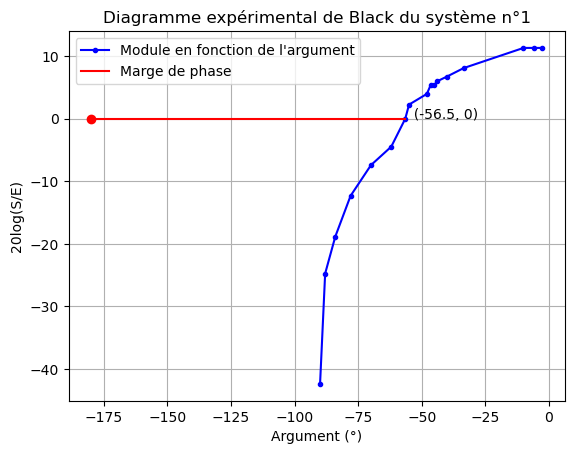
\includegraphics{TP1/Syst_1/Diagramme de Black experimental 2.1.png}
\end{center}

On remarque que ce diagramme a l'allure d'un passe-bas du $1^{er}$ ordre ($A > 0$, $\varphi \in [0^\circ,-90^\circ]$).
\\Graphiquement, la marge de phase (écart en phase entre le point à -180° et la courbe lorsque le gain est nul (sur l’axe des abscisses)) vaut $-56.5 - (-180) = 123.5^\circ$. Nous pouvions déjà déterminer la marge de phase sans le diagramme car nous avions déjà trouvé la fréquence pour laquelle $\frac{S}{E} = 1$.
\\Il suffit ensuite de mesurer le déphasage pour cette fréquence et d'y additionner 180.
\newpage


\begin{itemize}
    \item Système 2
\end{itemize}

\underline{Nature du système} : De même que pour le système 1, à fréquences très basse ($f \approx 10$Hz), l'amplitude de la sortie est amplifiée, et pour des fréquences très élevées, l'amplitude de la sortie est quasiment nulle.
\\De plus, on remarque que pour $f = 5$Hz, le quotient de l'amplitude de la sortie (S) sur celle de l'entrée est supérieur ($\frac{S}{E} = 2.26$) que pour $f = 1$Hz ($\frac{S}{E} = 2$). On interpète ceci comme étant une résonance du système autour de la fréquence 5 Hertz.
Ainsi le système 2 est un passe-bas du $2^{\grave{e}  me}$ ordre. Pour déterminer la fréquence de coupure, nous savons qu'à cette fréquence, pour un filtre passe-bas du $2^{\grave{e}me}$ ordre, le déphasage vaut $-90^\circ$ ($A = 2 > 0$). Ainsi, on trouve $f_0 \approx 7.57$Hz donc $\omega_0 \approx 47.5$Hz.

Nous pouvons désormais mesurer les différents points nécessaires pour tracer le diagramme de
Black :
Comme nous avons déjà un ordre de grandeur de la pulsation de coupure, nous mesurons le module
et l’argument à des fréquences séparées par des intervalles plus petits lorsque ces fréquences sont
proches de $\omega_0$ et on agrandit les intervalles lorsqu’on s’en éloigne.
\begin{center}
    \begin{tabular}{ |p{3cm}|p{3cm}|p{3cm}|p{3cm}| }
        \hline
        \multicolumn{4}{|c|}{Points du diagramme de Black du système 2} \\
        \hline
        Fréquence $f$(Hz) & $\mid T \mid = \frac{S}{E}$ & $20 \log(\mid T \mid)$ & Déphasage $\varphi $ (°)\\
        \hline
        0.5 & 1.95 & 13.36 & -2.51 \\
        0.6 & 1.95 & 13.36 & -4.70 \\
        1.2 & 2 & 13.86 & -9.32 \\
        2 & 2.024 &  14.10 & -15.95 \\
        3 & 2.1 &  14.84 & -25.33 \\
        4 & 2.14 &  15.22 & -36.80   \\
        5 & 2.26 & 16.31 & -49.80 \\
        6 & 2.21 & 15.86 & -65.47 \\
        7 & 2.02 & 14.06 & -82.9\\
        \hl{$7.55 = f_0$} & 1.95 & 13.36 & -90\\
        8 & 1.83 &  12.09 & -97 \\
        10 & 1.30 &  5.25 & -118.5 \\
        11.5 & 1 & 0 &-130 \\
        15 & 0.57 & -11.24 & -145 \\
        25 & 0.24 & -28.54 & -161 \\
        35 & 0.14 & -39.32 & -166 \\
        50 & 0.07 & -53.19 & -170 \\
        100 & 0.023 & -75.45 & -175 \\
        \hline
        \end{tabular}
    \end{center}

    \newpage

    Voici le diagramme de Black expérimental : 
    \begin{center}
        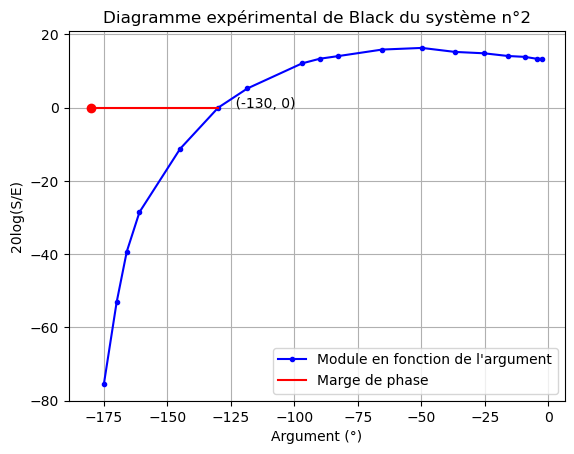
\includegraphics{TP1/Syst_2/Diagramme de Black experimental_syst2.png}
    \end{center}
    On remarque que ce diagramme a l'allure d'un passe-bas du $2^{\grave{e}me}$ ordre ($A > 0$, $\varphi \in [0^\circ,-180^\circ]$ et résonance).
    \\Graphiquement, la marge de phase vaut $-130 - (-180) = 50^\circ$.
\newpage
    \section{\itshape Réponse indicielle.Réponse Harmonique.Identification}

    Le but de cette partie est dde modéliser notre système par une fonction de transfert. Pour cela, nous allons effectuer un essai indiciel ou harmonique sur les deux systèmes.
    \subsection{\itshape Travail Préparatoire}
\begin{itemize}
    

    \item  \underline{\itshape Caractéristique statique} : Pour un système linéaire la caractéristique statique est une
    droite passant par l'origine, dans une zone linéaire la pente de cette droite est
    l'amplification statique du système.

    \item \underline{\bf \itshape Système du $1^{er}$ ordre} : Soit la fonction de transfert du $1^{er}$ ordre $F_1(p) = \frac{A}{1 + \tau p }$. Ici A représente le gain/l'amplification statique et $\tau$ représente la constante de temps (en secondes) du système.
    Pour représenter la réponse indicielle, nous savons que pour une entrée $e(t) = X_0\times\mathcal{U}(t)$, la réponse est de la forme $y(t) = AX_0(1-e^{\frac{-t}{\tau}})\mathcal{U}(t)$ avec $A$ et $\tau$ les éléments caractéristiques de $F_1(p)$.
    Ici, l'essai indiciel est modélisé avec A = 2, $X_0 = 1$ et $\tau = 0.2$s
    \begin{center}
        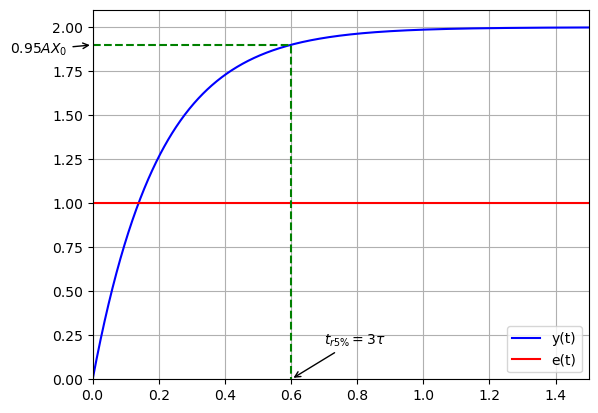
\includegraphics{TP1/Syst_1/Reponse_indicielle_prem_ordre.png}
    \end{center}
    Pour retrouver A: on fait le rapport entre l'allure de la sortie et l'allure de l'entrée en régime permanent.Pour retrouver $\tau$ : on mesure le temps de réponse à 5 $t_{r5\%}$(temps que met la sortie pour atteindre 95$\%$ 
    de sa valeur finale et y rester) et on retrouve $\tau$ grâce à la formule $t_{r5\%} = 3\tau$ (valable pour les systèmes du $1^{er}$ ordre).

    \textit{Fréquence d'observation}: pour bien observer l'allure de la sortie lorsqu'on fait un essai indiciel il faut choisir la bonne fréquence pour le signal carré d'entrée.
    \\ On doit pouvoir observer le régime transitoire et le régime permanent : si la fréquence est trop élevée on ne verra que le régime transitoire (régime permanent jamais atteint : bascule haut/bas trop
rapide) et si la fréquence est trop faible on ne verra pas le régime transitoire (il sera "écrasé" par le régime permanent). On doit donc prendre un demi-période de sorte à ce que la fréquence soit inférieure à $\frac{1}{3} \times f_0$ (car $t_{r5\%} = 3\tau$) mais pas trop pour observer le régime transitoire.
\\\\Lors d'un essai harmnonique, il suffit de mesurer la rapport de l'amplitude de la sortie sur celle de l'entrée à fréquence très basse comme ce système est un passe-bas du $1^{er}$ ordre. Pour déterminer $\tau$, on sait que à $\omega_0$, le déphasage $\varphi$ vaut $-45^\circ$. Ainsi en trouvant $\omega_0$, on trouve $\tau$ car $\omega_0 = \frac{1}{\tau}$.
\\\\\\\\
\item \underline{\bf \itshape Système du $2^{\grave{e}me}$ ordre} : Soit la fonction de transfert du $2^{\grave{e}me}$ ordre  $F_2(p) = \frac{A}{1 + 2m\frac{p}{\omega_0} + (\frac{p}{\omega_0})^2}$. 
\end{itemize}
Ici, A  représente le gain/l'amplification statique, m le coefficient d'amortissement du système et $\omega_0$ la pulsation de coupure du système.
Pour représenter la réponse indicielle, d'après le cours, nous savons que pour une entrée $e(t) = X_0\times\mathcal{U}(t)$, la réponse est de la forme  :

\begin{center}
    $y(t) = AX_0(1+A_1e^{p_1t} + A_2e^{p_2t})\mathcal{U}(t)$ 
\end{center}    
Avec $p_1$ et $p_2$ les pôles de la fonction de transfert, i.e. les racines du polynôme en p du dénominateur.
D'après le cours, si m $\ge 1$, alors $p_1 = \omega_0(-m+\sqrt{m^2-1})$ et $p_2 = \omega_0(-m-\sqrt{m^2-1})$. 
\\Et, de plus : $A_1 = \frac{\omega_0^2}{p_1(p_1-p_2)}$ et $A_2 = \frac{\omega_0^2}{p_2(p_2-p_1)}$.
Ainsi, pour A = 2, $X_0 = 1$ et $\omega_0 = 10$rad/s, on obtient le graphe suivant :
\begin{center}
    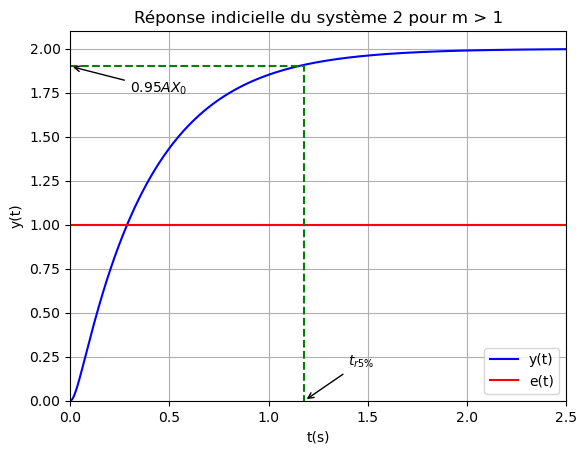
\includegraphics{TP1/Syst_2/Reponse_indicelle_m_sup_1.png}
\end{center}

On observe bien aussi la tangente nulle à l'origine, typique d'un système du deuxième ordre.

Pour $0\le m \le 1$, alors $p_1$ et $p_2$ sont complexes conjugués, i.e. $p_1 = \omega_0(-m+j\sqrt{1-m^2})$ et $p_2 = \omega_0(-m-j\sqrt{1-m^2})$.
On pose alors $p_1 = \alpha+j\beta$ et $p_2 = \alpha-j\beta$. Enfin, d'après le cours, on obtient : 
\begin{center}
    $y(t) = AX_0(1+2A_1e^{\alpha t}\cos(\beta t + \theta))\mathcal{U}(t)$
\end{center}
Avec $A_1 = |\underline{A_1}|$ car comme $p_1$ et $p_2$ sont des complexes, $\underline{A_1}$ l'est aussi.
On sait que : 
\begin{center}
 $\underline{A_1} = \frac{\omega_0^2}{\underline{p_1}(\underline{p_1} - \underline{p_2})} = \frac{\omega_0}{(\alpha + j\beta)(2j\beta)} = \frac{\omega_0}{2j\beta\alpha -2\beta^2}$
\\Il vient alors $A_1 = |\underline{A_1}| = \frac{\omega_0^2}{\sqrt{(-\beta^2)^2 + (2\beta\alpha)^2}}$
\\Après calcul, $\theta = \arg(\underline{A_1}) = \arctan(\frac{\Im(\underline{A_1})}{\Re(\underline{A_1})}) - \pi = \dots = \arctan(\frac{\alpha}{\beta^3}) - \pi$
\end{center}
On peut désormais tracer la réponse indicielle d'un système du deuxième ordre avec $m \in \left]0;1\right[$, $A = 2$, $\omega_0 = 10$rad/s, $X_0 = 1$  :
\begin{center}
    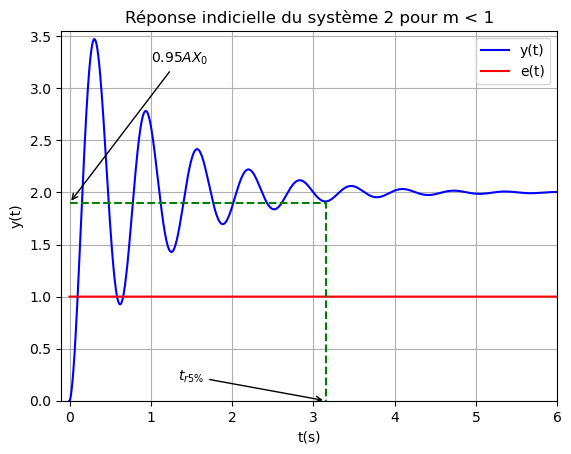
\includegraphics{TP1/Syst_2/Reponse_indicielle_m_inf_1.png}
\end{center}
\textit{Méthode de détermination des éléments caractéristiques :} On applique un signal carré en entrée, et on observe la réponse indicielle. 
\\Ensuite on mesure le $1^{er}$ dépassement (en $\%$ ) et on utilise l'abaque qui nous permet de relier le pourcentage du premier dépassement au coefficient d'amortissement.
\\Enfin, grâce à un deuxième abaque, on peut récupérer le temps de réponse réduit ($t_{r5\%}\omega_0$) avec le coefficent d'amortissement. Comme la pulsation de coupure est connue, on peut récupérer le temps de réponse à 5 $\%$.
\\\\$\underline{F_2}(j\omega_0) = \frac{A}{1 + 2m\frac{j\omega_0}{\omega_0} + (\frac{j\omega_0}{\omega_0})^2} = \frac{A}{2jm}$

\begin{itemize}
            \item $|\underline{F_2}(j\omega_0)| = \frac{A}{2m}$
            \item $\arg(\underline{F_2}(j\omega_0)) = -90^\circ$
\end{itemize}

Grâce à ces résultats, on peut extraire une méthode pour trouver $m$ et $\omega_0$ lors d'un essai harmonique: 
Faire varier la fréquence jusqu'à obtenir un déphasage de $-90^\circ$. Alors la fréquence qui correspond à ce déphasage est la fréquence de coupure $f_0$. 
\\Donc $\omega_0 = 2\pi f_0$. De plus, on sait qu'à la pulsation de coupure, l'amplification vaut $\frac{A}{2m}$. Il suffit de mesurer $\frac{S}{E}$ à cette pulsation et on peut en déduire m :
\begin{center}
    $\frac{S}{E} = \frac{A}{2m} \Leftrightarrow m = \frac{A}{2}\times \frac{1}{\frac{S}{E}}$
\end{center}

\subsection{\itshape Travail expérimental}

\subsubsection{\underline{\textit{Tracé de la caractéristique statique} }}
Comme dit dans l'énoncé de TP, nous appliquons un signal carré de très faible fréquence(500mHz) et on mesure la sortie  lorsque celle-ci atteint son régime permanent pour plusieurs valeurs d'entrée : 

\begin{itemize}
    \item \bf \large Système 1
\end{itemize}
\begin{center}
    \begin{tabular}{ |p{3cm}|p{3cm}|}

        \hline
        Amplitude d'entrée (V) & Amplitude de sortie (V)\\
        \hline
        -9.25 & -12.4 \\
        -8.25 & -12.6\\
        -7.25 & -12.4  \\
        -6.25 & -10.9 \\
        -5.25 & -9  \\
        -4.2 & -7.4  \\
        -3.15 & -5.5\\
        -2.05& -3.65  \\
        -2 & -3.65\\
        -1.55 & -2.75 \\
        0.95 & 2.72 \\
        1.45 & 3.60 \\
        2 & 3.65 \\
        2.95 & 5.5 \\
        3.95 & 7.325  \\
        4.875 & 9  \\
        5.8 & 10.9  \\
        7 & 12.8  \\
        7.87 & 12.8  \\
        9 & 12.8  \\
        
        \hline
        \end{tabular}
    \end{center}

    Et voici le tracé de la caractéristique statique :
    \begin{center}
        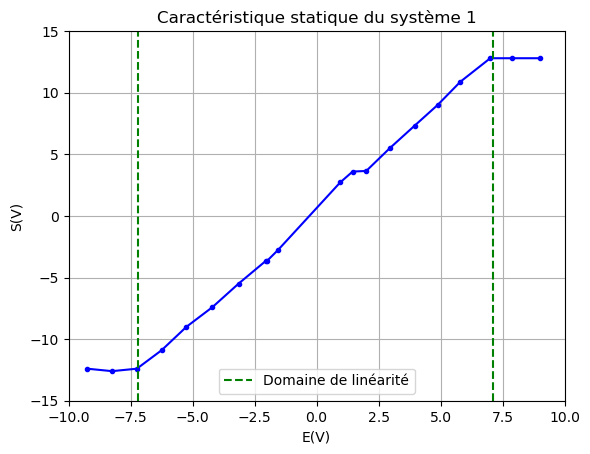
\includegraphics{TP1/Syst_1/Carac_stat_1.png}
    \end{center} 
    Grâce à cette caractéristique statique, on peut mesurer l'amplification statique, qui est la pente de \\la droite dans le domaine de linéarité ($D = \left[-7.4;7.3\right]$), qui est délimité par les pointillés en vert. On voit clairement sur le graphe que $A\approx1.8$, ce qui confirme nos résultats précédents.
    \\On peut confirmer ceci en calculant le coefficient directeur entre les points $(2.95,5.5)$ et  $(-2,-3.65)$. Ainsi $A = \frac{5.5-(-3.65)}{2.95-(-2)} = 1.84 \approx 1.8$.
   \\De plus, on peut expliquer le domaine de linéarité par le fait que les composants du système 1 (Amplificateurs opérationnels) on une tension $V_{sat}$ de saturation maximale. Si on met en entrée une tension trop élevée, l'AOP ne pourra pas l'amplifier assez vite et la sortie ne pourra pas dépasser $V_{sat}$.
\newpage
    \begin{itemize}
    \item \bf \large Système 2
\end{itemize}
\begin{center}
\begin{tabular}{ |c|c|c|c|c|c|c|c|c|c|c|c|c|}

    \hline
    Amplitude d'entrée (V) & -8.3&-6.25&-5.2&-4.2&-2&-1&1&1.9&3.75&4.8&5.75&7.93\\
    \hline
    Amplitude de sortie (V) & -12.4&-12&-10&-8&-4&-1.53&1.475&4&8&10&12&12.8\\
    \hline
    \end{tabular}
\end{center}
Et voici le tracé de la carctéristique statique : 

\begin{center}
    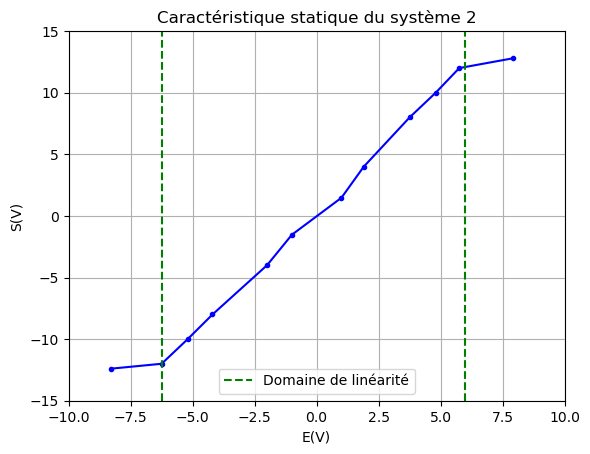
\includegraphics{TP1/Syst_2/Carac_stat_2.png}
\end{center}
Grâce à cette caractéristique statique, on peut mesurer l'amplification statique, qui est la pente de \\la droite dans le domaine de linéarité ($D = \left[-6.25;6\right]$), qui est délimité par les pointillés en vert. On voit clairement sur le graphe que $A\approx2$, ce qui confirme nos résultats précédents.
\\On peut confirmer ceci en calculant le coefficient directeur entre les points $(4.8;10)$ et  $(-6.25,-12)$. Ainsi $A = \frac{10-(-12)}{4.8-(-6.25)} = 1.99 \approx 2$. Le domaine de linéarité est expliqué par les mêmes raisons que pour le système 1.
\newpage
\subsubsection{\underline{\itshape Identification}:}
\begin{itemize}
    \item \bf \large Système 1
\end{itemize}
\textit{\underline{Essai indiciel:}} On applique un signal carré de fréquence 1Hz et d'amplitude 1V pour mesurer l'amplification statique et un signal carré de fréquence 15Hz de façon à observer à la fois le régime transitoire et le régime permanent, voici ce que l'on obtient :
\begin{center}
    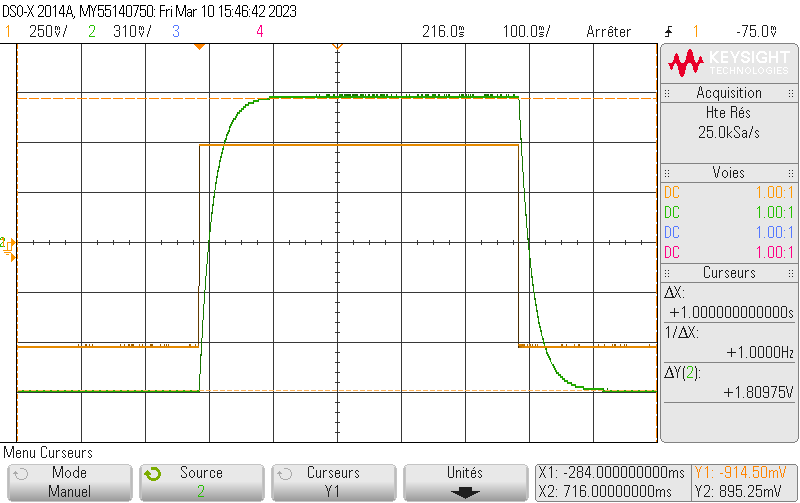
\includegraphics[width = 17 cm, height = 10cm]{TP1/Syst_1/Ampli_statique__syst_1.png}
    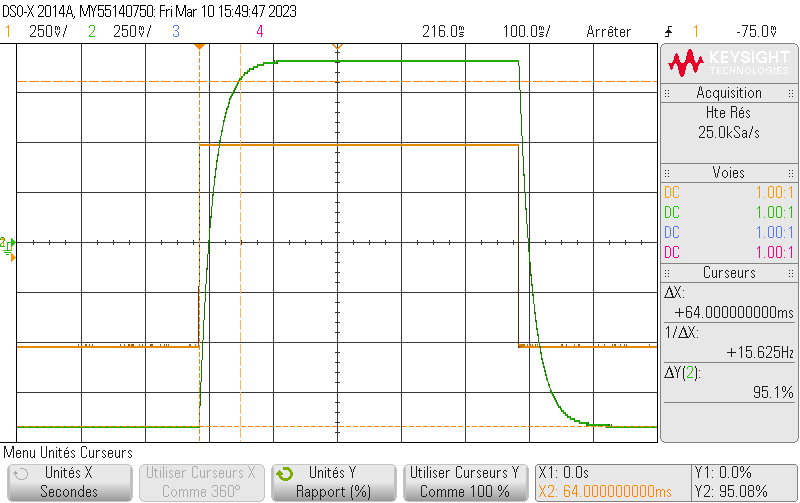
\includegraphics[width = 17 cm, height = 10cm]{TP1/Syst_1/tr5prct_syst_1_indiciel.png}
\end{center}

\begin{itemize}
    \item A : D'après le la première capture et des curseurs, avec $V_s$ en vert et $V_e$ en orange on a :
    \\$A = \frac{\Delta S}{\Delta E} = \frac{1.81}{1} = 1.81$ qui correspond à la valeur que nous avons trouvée grâce à la carctéristique statique.
    \item $\tau$ : D'après la seconde capture, le temps de réponse à 5 $\%$ est de 64ms (voir $\Delta X$ dans l'onglet "Curseurs"). 
    \\Or comme le système étudié est d'ordre 1, alors on sait aussi que :
    \\$t_{r5\%} = 3\tau \Leftrightarrow \tau = \frac{t_{r5\%}}{3} = \frac{64}{3} = 21.3$ms.
\end{itemize}
\begin{center}
Ainsi on a \fbox{$F_1(p) = \frac{1.81}{1+0.0213p}$}

\end{center}

\underline{\itshape Essai harmonique:} Similairement à la section 2.2, on retrouve A à très basse fréquence en faisant l'opération suivante : $A = \frac{\Delta S}{\Delta E} = 1.79 \approx 1.81$ qui est la même valeur qu'à l'essai indiciel.
De plus, à un déphasage $\varphi$ de $-45^\circ$, on trouve la pulsation de coupure $f_0 = 7.5$Hz donc $\omega_0 = 2\pi f_0 = 47.12$ rad/s or $\tau = \frac{1}{\omega_0} = 0.0212$s qui correspond à la valeur de $\tau$ trouvée grâce à l'essai indiciel.

\begin{itemize}
    \item \bf \large Système 2
\end{itemize}
\underline{\itshape Essai indiciel:} On applique un signal carré de fréquence 2Hz et d'amplitude 1V pour observer le régime transitoire et le régime permanent. On mesure ensuite l'amplitude du premier dépassement: 
\begin{center}
    
    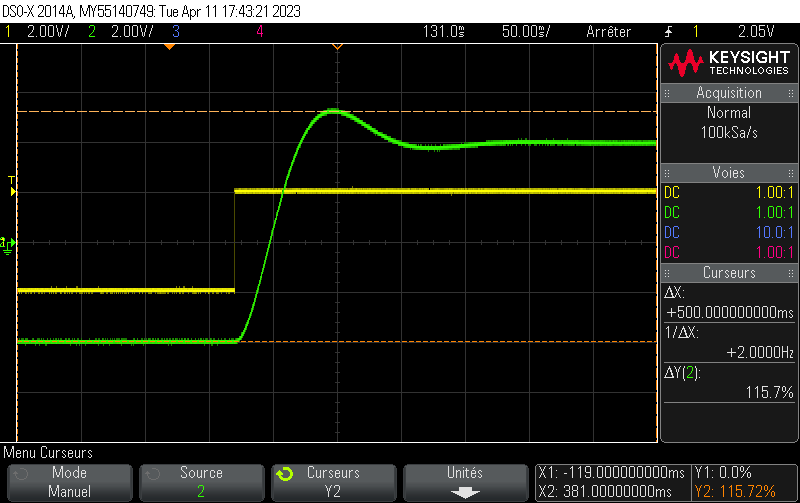
\includegraphics[width = 17cm, height = 11 cm]{TP1/Syst_2/Depassement_syst_2.png}
    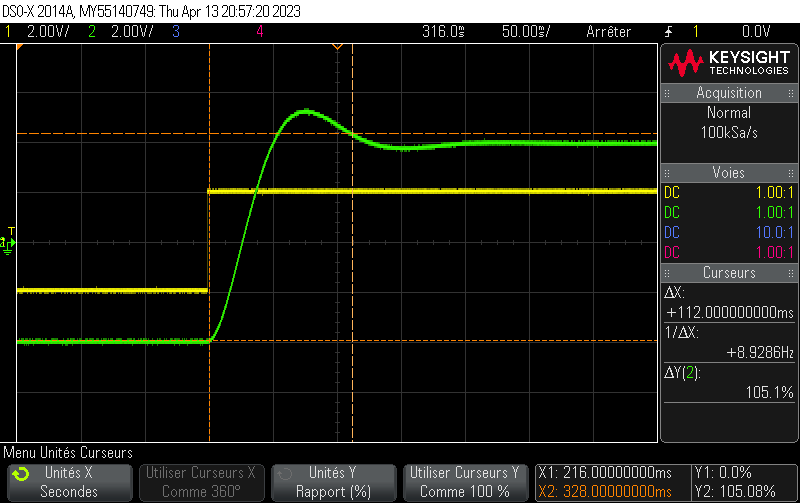
\includegraphics[width = 17cm, height = 11 cm]{TP1/Syst_2/13_04_23_tr5prct_2.png}
\end{center}
On observe donc que le premier dépassement dépasse de 15.7$\%$ la valeur finale. Il suffit ensuite d'utiliser l'abaque qui relie l'amplitude du premier dépassement au coefficient d'amortissement. Nous trouvons \fbox{$m = 0.5$}.
De plus avec le deuxième abaque et le temps de réponse à 5$\%$ (deuxième capture d'écran, $t_{r5\%} = 112$ms), on récupère le temps de réponse à 5$\%$ réduit :
\\ $t_{r5\%}\omega_0 = 5 \Leftrightarrow $ \fbox{$\omega_0 = \frac{5}{112.10^{-3}} = 44.6$ rad/s}.
\begin{center}
    Ainsi on a \fbox{$F_2(p) = \frac{2}{1 + \frac{p}{44.6} + (\frac{p}{44.6})^2}$}.

\end{center}

\underline{\itshape Essai harmonique:} Similairement à la section 2.2, on retrouve A à très basse fréquence en effectuant l'opération suivante :
\\$A = \frac{\Delta S}{\Delta E} = 2.008 \approx 2$ qui est la même valeur qu'à l'essai indiciel. De plus, à un déphasage $\varphi$ de $-90^\circ$, on trouve la pulsation de coupure $f_0 = 7.57$Hz, donc $\omega_0 = 2\pi f_0 = 47.4$ rad/s.
Mais on sait aussi qu'à $\omega_0$, $\frac{S}{E} = \frac{A}{2m}$ or $\frac{S}{E} = 2$ à $\omega_0$ donc finalement, on obtient $1 = \frac{1}{2m} \Leftrightarrow m = 0.5$ ce qui confirme nos résultats suite à l'essai indiciel.

\newpage

\section{\itshape Calcul d'un correcteur et simulations}

Nous avons désormais identifié les mesuré les éléments caractéristiques des deux systèmes. Cependant ces systèmes ne sont pas encore asservis. Désormais nous allons calculer un correcteur qui permettra d'asservir nos deux systèmes.
\\On désire asservir le système suivant : 
\begin{center}
    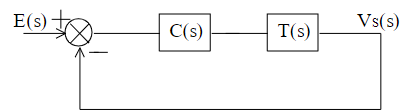
\includegraphics{TP2 Simulink/syst_a_asservir.png}
\end{center}

\subsection{\itshape Système 1}
\subsubsection{\underline{\itshape \bf Correcteur proportionnel}}
On considère dans un premier temps un correcteur proportionnel $C(p) = K > 0$ et le système 1 qui est modélisé par une fonction de transfert du premier ordre $T(s) = F_1(s) = \frac{A}{1 + \tau p}$.
\\
\begin{itemize}
    \item Calculons la Fonction de Transfert en Boucle Fermée (FTBF) grâce à la formule de Black : 
\end{itemize}

\large $FTBF = \frac{K\times \frac{A}{1 + \tau p}}{1 + K\times \frac{A}{1 + \tau p}} = \frac{KA}{1 + \tau p + KA} = \frac{\frac{KA}{1 + KA}}{1 + \frac{\tau}{1 + KA}p} = \frac{K_{BF}}{1 + \tau_{BF}p}$
\begin{itemize}
    \item \normalsize Calculons désormais l'erreur statique et le temps de réponse à 5$\%$ : 
\end{itemize}
\normalsize D'après le théorème de la valeur finale : 
\\
\large $\epsilon_s = \lim_{t \to \infty} \epsilon(t) = \lim_{p \to 0}p\epsilon(p)$
\normalsize or \large $\frac{\epsilon(p)}{E(p)} = \frac{1}{1 + \frac{KA}{1 + \tau p}}$ et $E(p) = \frac{E_0}{p}$ \normalsize donc en injectant :
\large$\epsilon_s = \lim_{p \to 0}p\times \frac{E_0}{p}\times \frac{1}{1 + \frac{KA}{1 + \tau p}} = \frac{E_0}{1 + KA}$
\\ \normalsize Application numérique pour $K=1$ et $A = 1.81$ :  $\epsilon_s =\frac{E_0}{1 + 1.81} = 0.35E_0 =$ \fbox{$35\%$}
\\
\begin{itemize}
    \item Pour un système du premier ordre, le temps de réponse à 5 $\%$ vaut $3\tau$, en particuler ici : $t_{r5\%} = 3\tau_{BF} = \frac{3\tau}{1 + KA} = \frac{3\times0.0213}{1 + 1.81} =$ \fbox{$22.74$ms}
\end{itemize}
On remarque que le temps de réponse à cinq pourcents du système  1 est trois fois plus rapide en étant bouclé que en boucle ouverte. Cependant, l'erreur statique est ici de 35$\%$ ce qui n'est pas du tout satisfaisant. 
\\Cherchons les valeurs de K pour que le système admette une erreur statique de 10$\%$ puis 1$\%$ et leurs temps de réponse à 5$\%$ correspondants : 
\\On cherche $\epsilon_s = 10\%$. Autrement dit : $\epsilon_s = 0.1E_0$. Mais aussi d'après les calculs précédents : 
\\$\epsilon_s = \frac{E_0}{1 + KA} = 0.1E_0 \Leftrightarrow 1 + K\times 1.81 = 10 \Leftrightarrow K = 4.97$

Pour $K = 4.97$, $t_{r5\%} = 3\tau_{BF} = 6.39$ms
\\\\On cherche $\epsilon_s = 1\%$. De la même manière, on trouve $K = 54.7$ et $t_{r5\%} = 0.64$ms

\begin{itemize}
    \item On désire avoir un système 5 fois puis 50 fois plus rapide qu'en boucle ouverte : calculons les valeurs de K correspondantes : 
\end{itemize}

Système 5 fois plus rapide $\Leftrightarrow$ \large$ t_{r5\%_{BF}} = \frac{t_{r5\%_{BO}}}{5}$ \normalsize $\Leftrightarrow$ \large $\frac{3\tau}{1 + KA} = \frac{3\tau}{5}$ \normalsize $\Leftrightarrow$ \large $K = 2.2$
\\\normalsize Donc pour $K = 2.2$, on trouve $t_{r5\%_{BF}} = 12.8$ms
\\\\\normalsize Erreur statique : \large $\epsilon_s = \frac{E_0}{1 + 2.2\times 1.81} = 0.2E_0 = 20\%$
\\\\\normalsize Système 50 fois plus rapide $\Leftrightarrow$ \large$ t_{r5\%_{BF}} = \frac{t_{r5\%_{BO}}}{50}$ \normalsize $\Leftrightarrow$ \large $\frac{3\tau}{1 + KA} = \frac{3\tau}{50}$ \normalsize $\Leftrightarrow$ \large $K = 27.2$
\\\normalsize Donc pour $K = 27.2$, on trouve $t_{r5\%_{BF}} = 1.27$ms
\\\\\normalsize Erreur statique : \large $\epsilon_s = \frac{E_0}{1 + 27.2\times 1.81} = 0.02E_0 = 2\%$
\\\\
\normalsize Résumons ainsi ces calculs sous forme de tableau : 

\begin{center}
    \begin{tabular}{ |p{3cm}|p{3cm}|p{3cm}|}

        \hline
        $K$ & $t_{r5\%}$(ms) & $\epsilon_s$ ($\%$)\\
        \hline
        1 & 22.74 & 35\\
        4.97 & 6.39 & 10\\
        54.7 & 0.64 & 1\\
        2.2& 12.8 & 20\\
        27.2 & 1.27  & 2\\
        
        
        \hline
        \end{tabular}
    \end{center}
\newpage 
\large \textit{ \textbf{Simulation}}
\\\\\normalsize Dans cette partie, nous avons utilisé le logiciel "Simulink" pour tracer la réponse indicielle de l'asservissement pour les cinq valeurs de K calculées précédemment. Nous avons utilisé ce système pour les différentes simulations : 
\begin{center}
    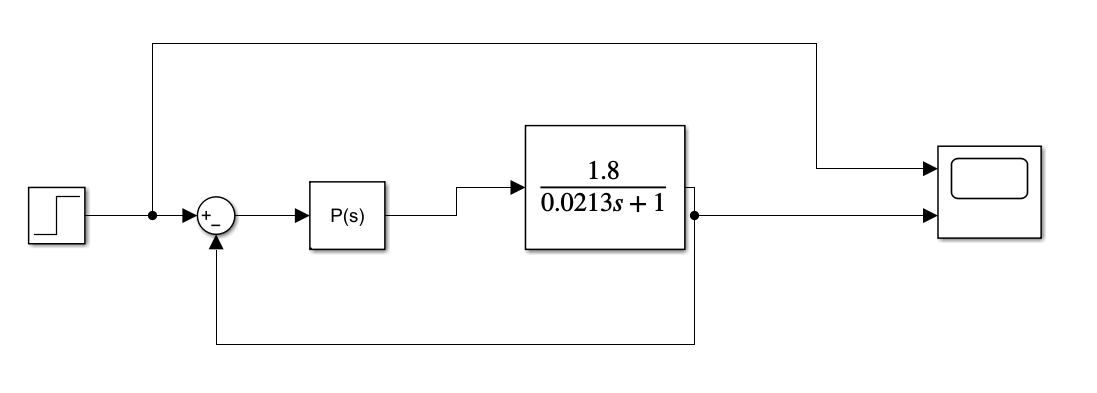
\includegraphics[width = 15 cm]{TP2 Simulink/Syst_1/Syst_1_Simulink_P.png}
\end{center}


\begin{itemize}
    \item \bf \large K = 4.97
\end{itemize}
\begin{center}
    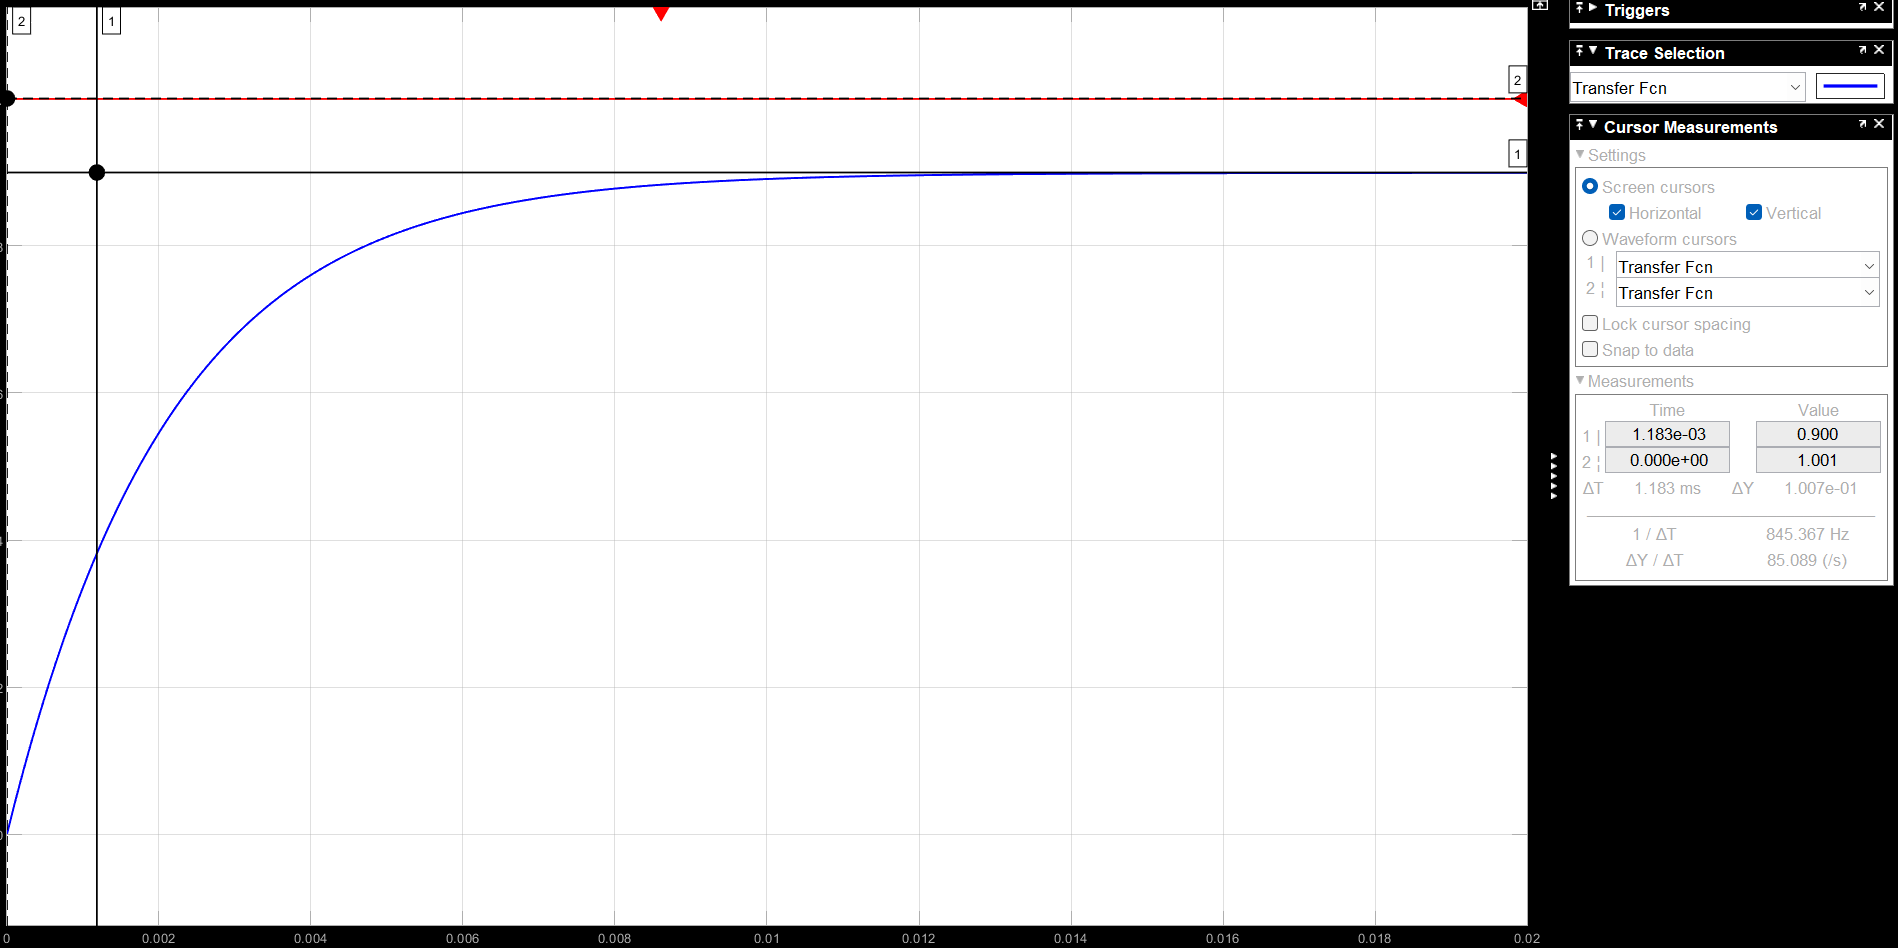
\includegraphics[width = 19 cm]{TP2 Simulink/Syst_1/Erreur statique_syst_1_K=4.97.png}
    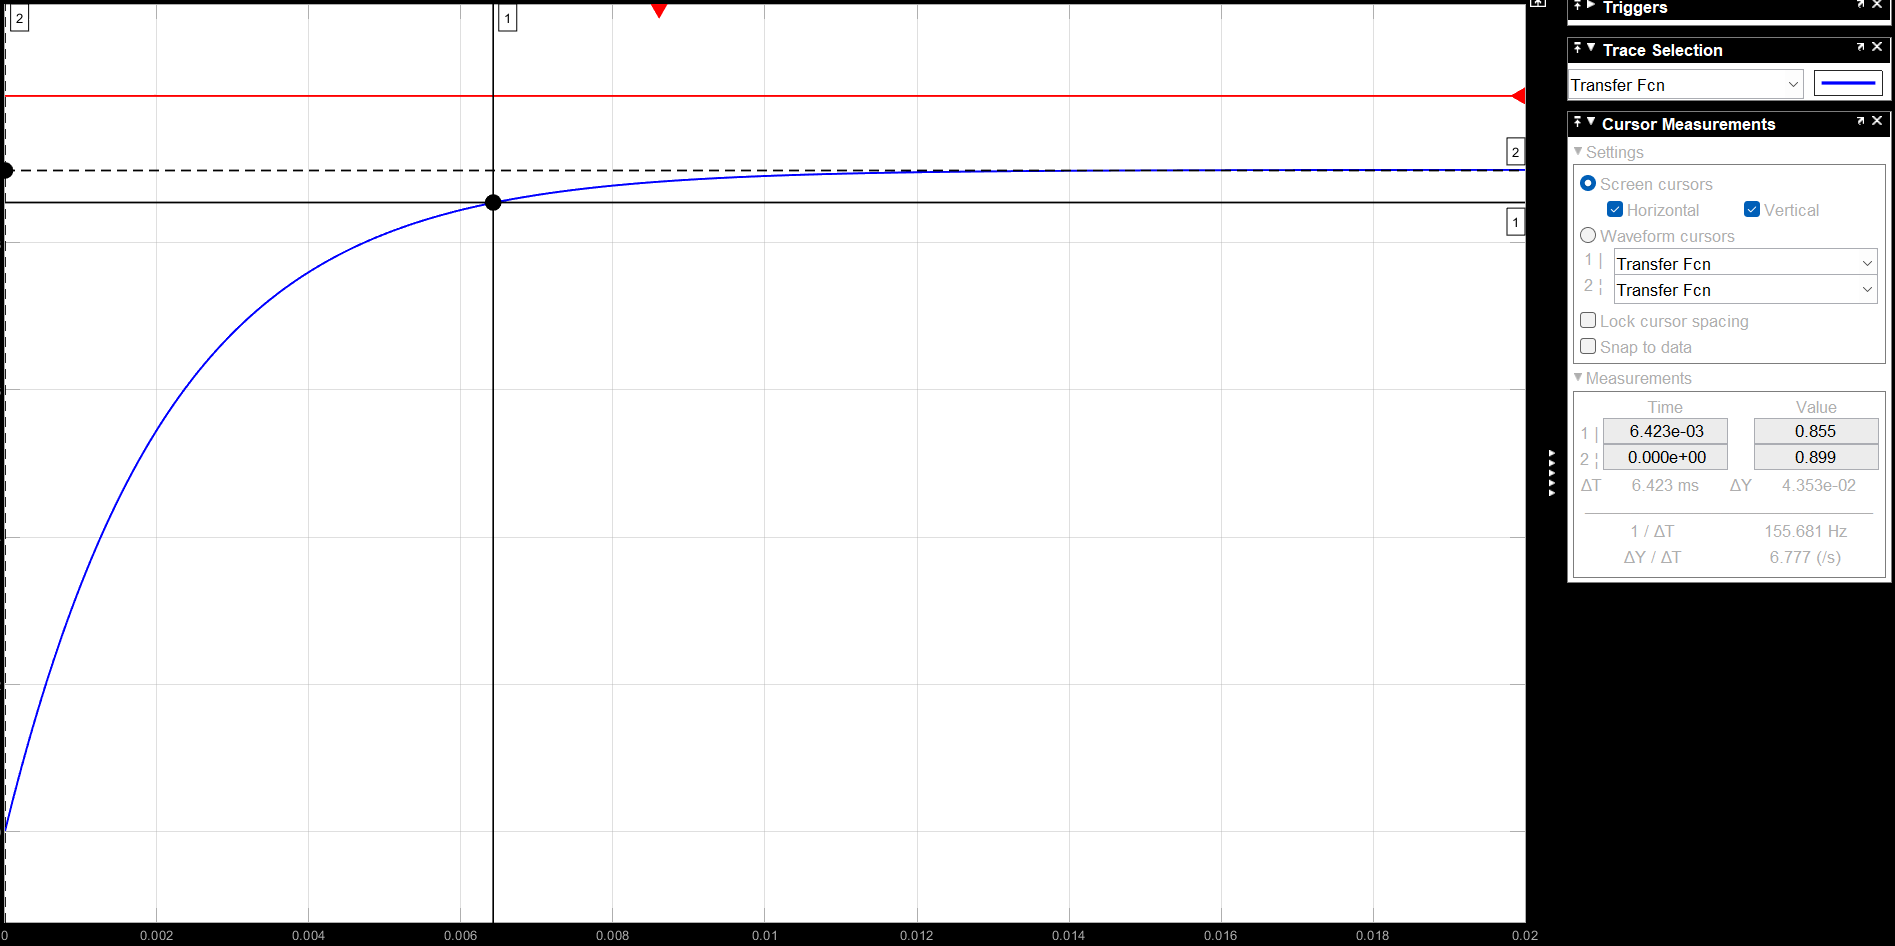
\includegraphics[width = 19 cm]{TP2 Simulink/Syst_1/Reponse_indic_syst_1_K=4.97_tr5prct.png}

\end{center}

\normalsize L'erreur statique est représentée comme étant l'écart entre les deux curseurs horizontaux sur le premier graphe. On lit grâce aux valeurs du curseur que l'échelon atteint 1 et la réponse indicielle atteint 0.9 en régime permanent (la simulation est assez longue pour voir le régime permanent). L'erreur statique est donc de 10$\%$ en lisant la valeur de $\Delta Y$ et en multipliant par 100 cett valeur pour l'avoir en pourcent.
\\De plus, on peut lire le temps de réponse à 5$\%$ sur le deuxième graphe : en effet, nous avons placé un curseur horizontal à 95$\%$ de la valeur finale de la réponse indicielle soit à $0.95\times0.9 = 0.855$.
Il suffit ensuite de placer un premier curseur vertical au tout début de la simulation (ici à $t=0$) et d'en mettre un deuxième au niveau du croisement entre la réponse indicielle et le curseur horizontal. On trouve graphiquement $t_{r5\%} = 6.42$ms en lisant la valeur de $\Delta T$.
\\Ainsi les valeurs trouvées en simulation sont quasiment égales (écart nul entre les erreurs statiques et écart de 0.03 ms entre les deux temps de réponse soit un écart de 0.46$\%$ qui peut s'expliquer par de légères erreurs de lecture graphique).
\newpage
\begin{itemize}
    \item \bf \large K = 54.7
\end{itemize}
\begin{center}
    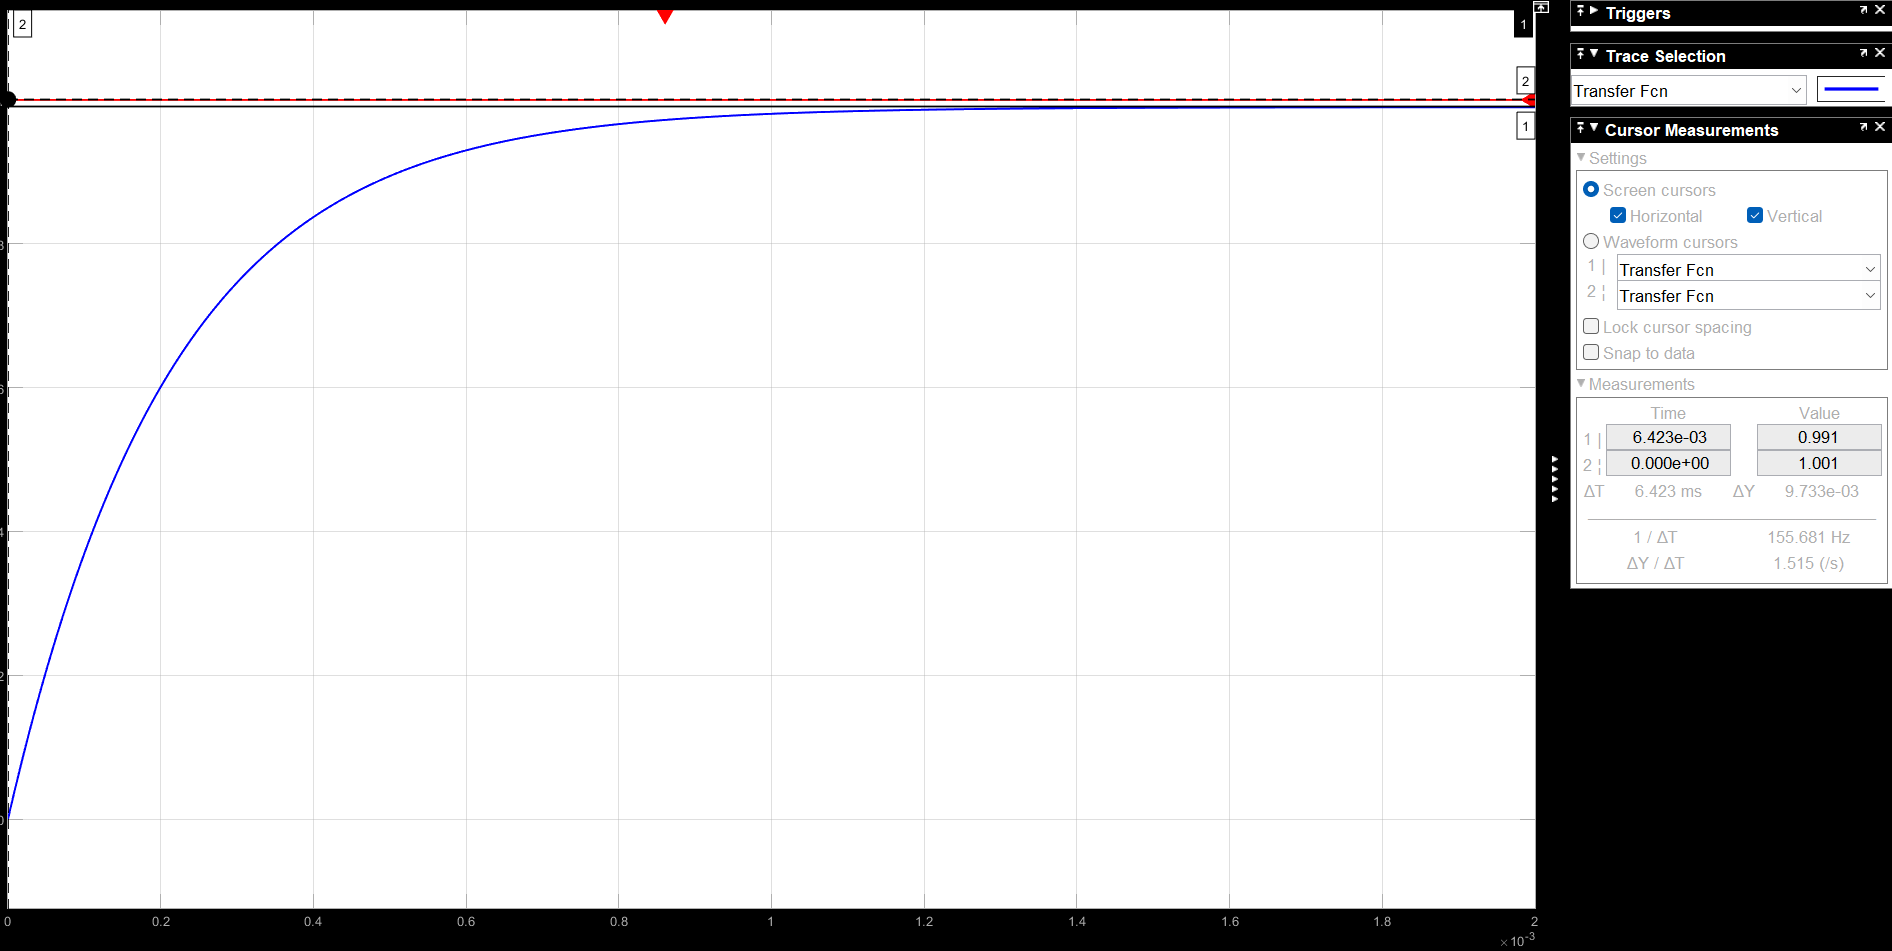
\includegraphics[width = 19 cm]{TP2 Simulink/Syst_1/Erreur_statique_syst_1_K=54.7.png}
    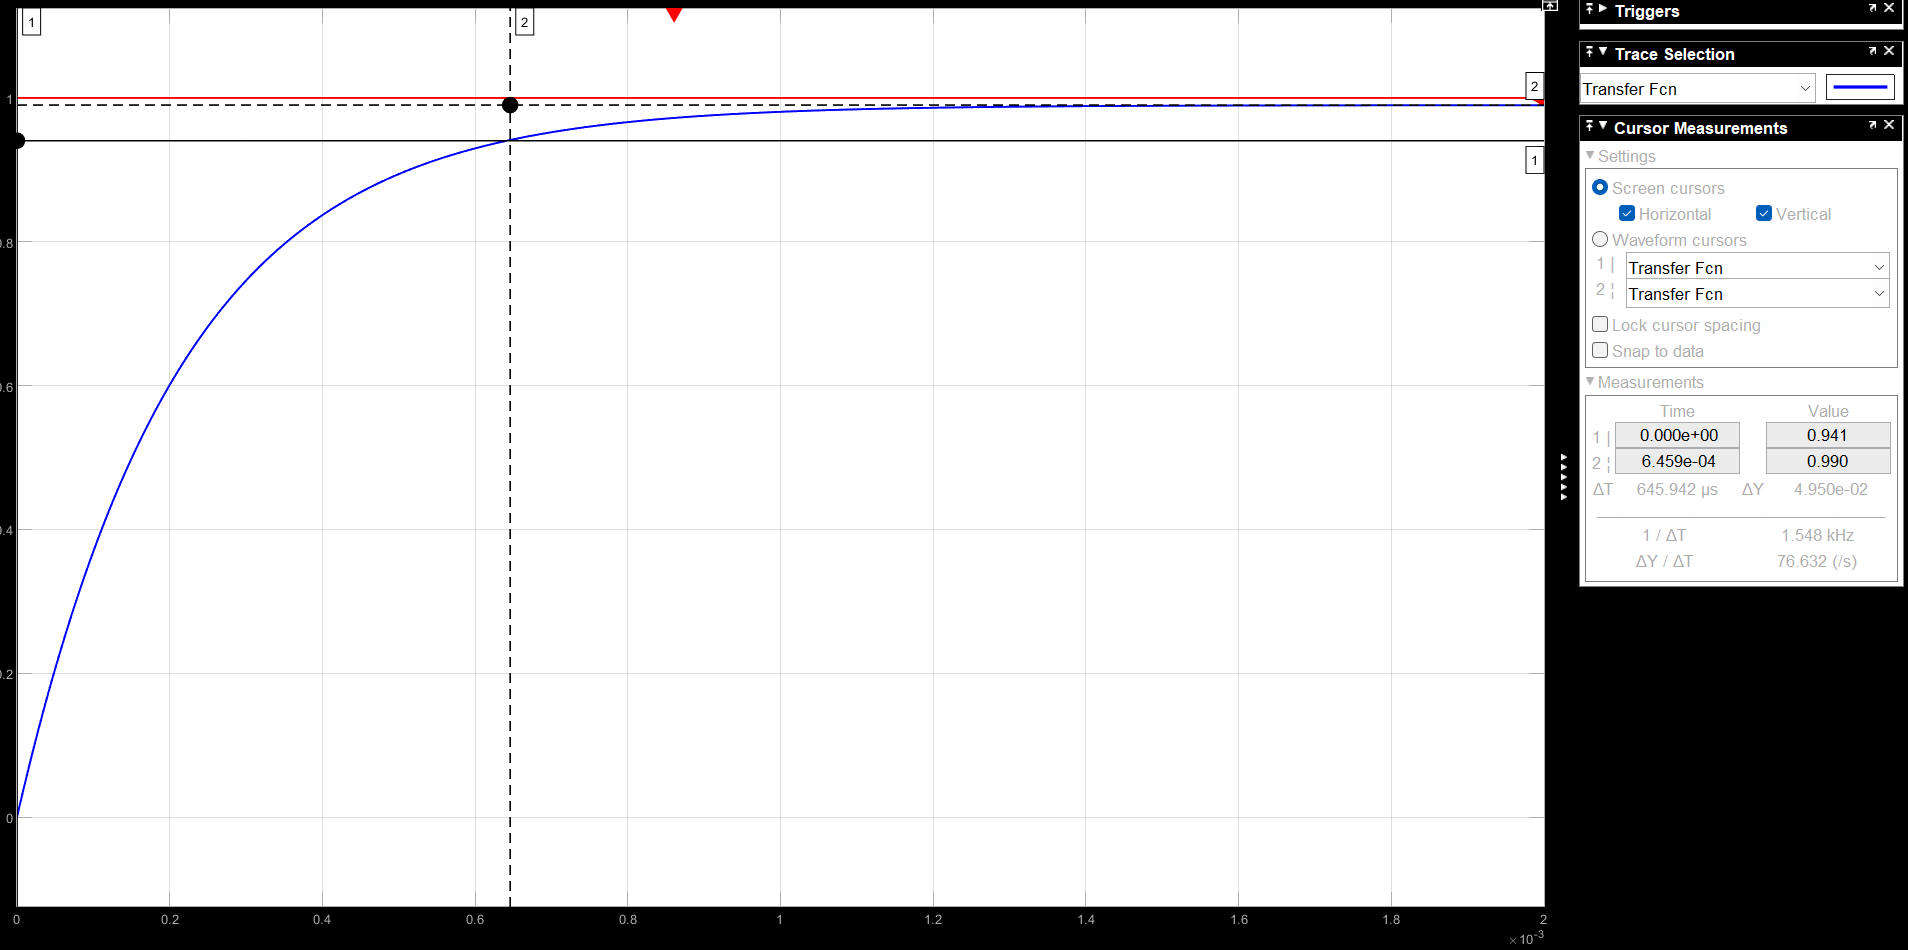
\includegraphics[width = 19 cm]{TP2 Simulink/Syst_1/tr5prct_syst_1_K=54.7.png}
\end{center}
\normalsize Par la même méthode que précédemment, on trouve comme erreur statique $0.9733\%$ et comme de temps de réponse à cinq pourcents de $0.646$ms.
\\Cette fois-ci, on attendait une erreur statique de 1$\%$ mais la valeur mesurée est légèrement inférieure de 2.67$\%$. Cette différence s'explique de la difficulté d'être précis pour mesurer une erreur statique de 1$\%$ sur le graphe.

\begin{itemize}
    \item \bf \large K = 2.2
\end{itemize}
\begin{center}
    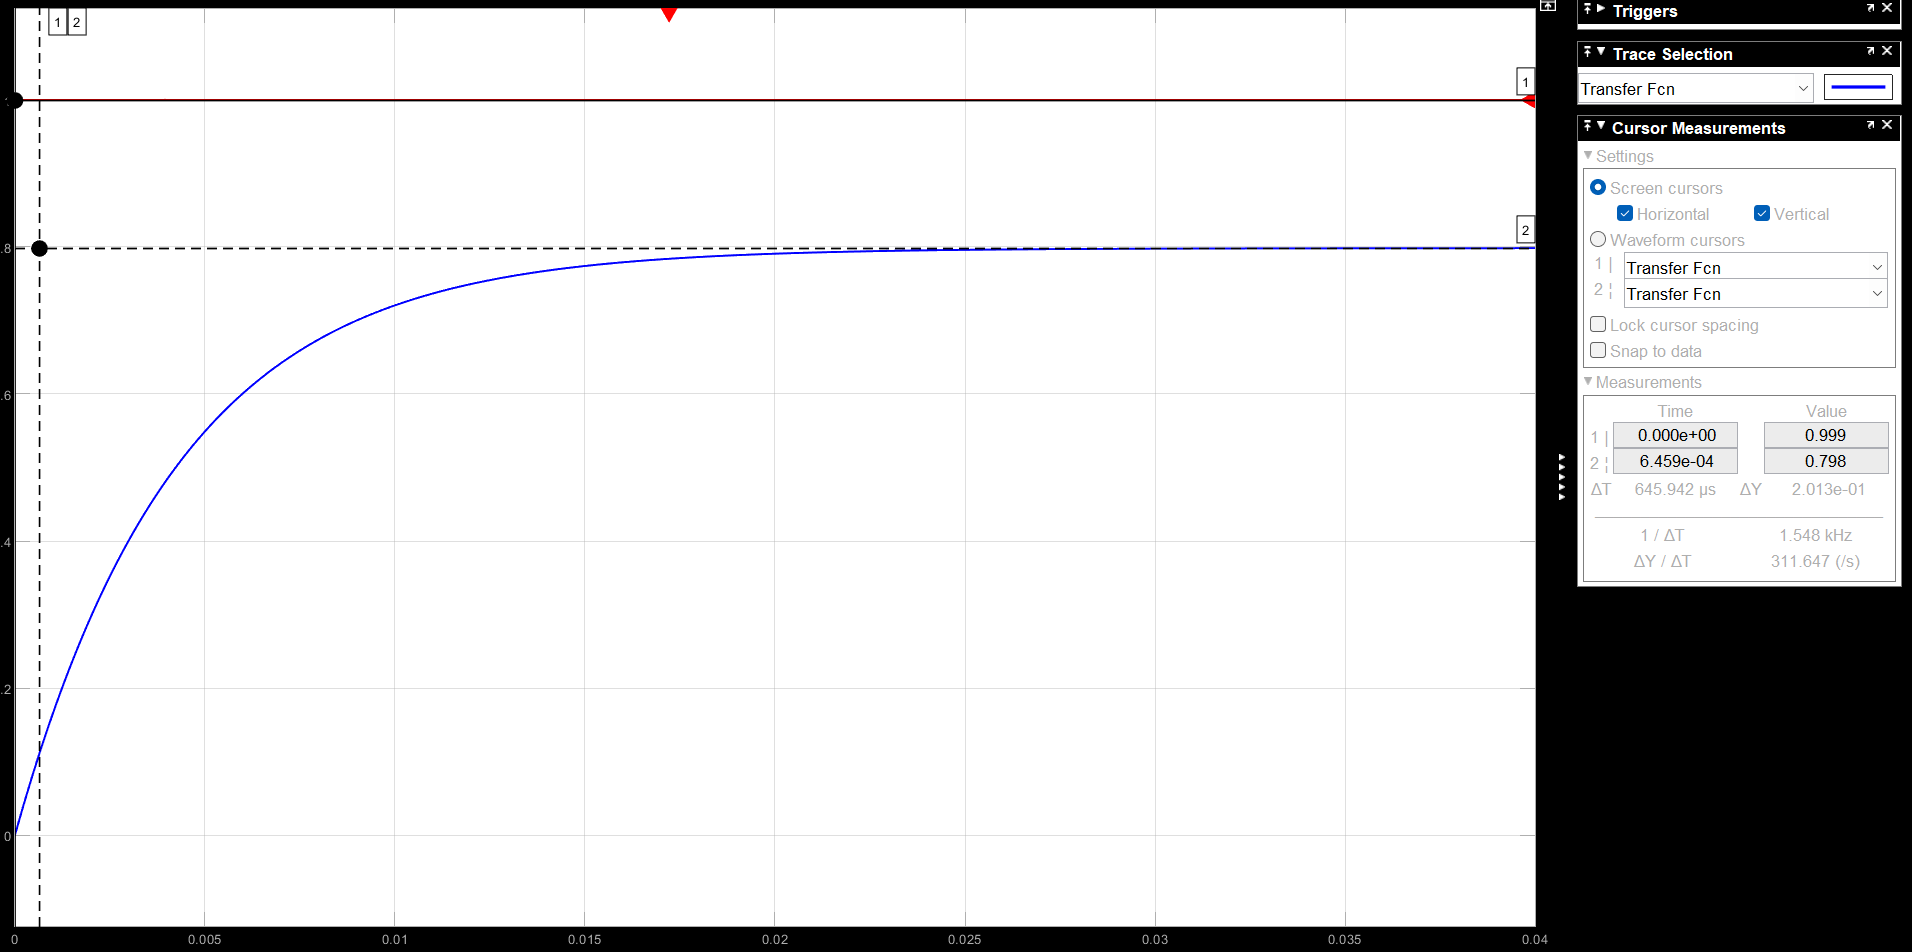
\includegraphics[width = 19 cm]{TP2 Simulink/Syst_1/Err_statique_syst_1_K=2.2.png}
    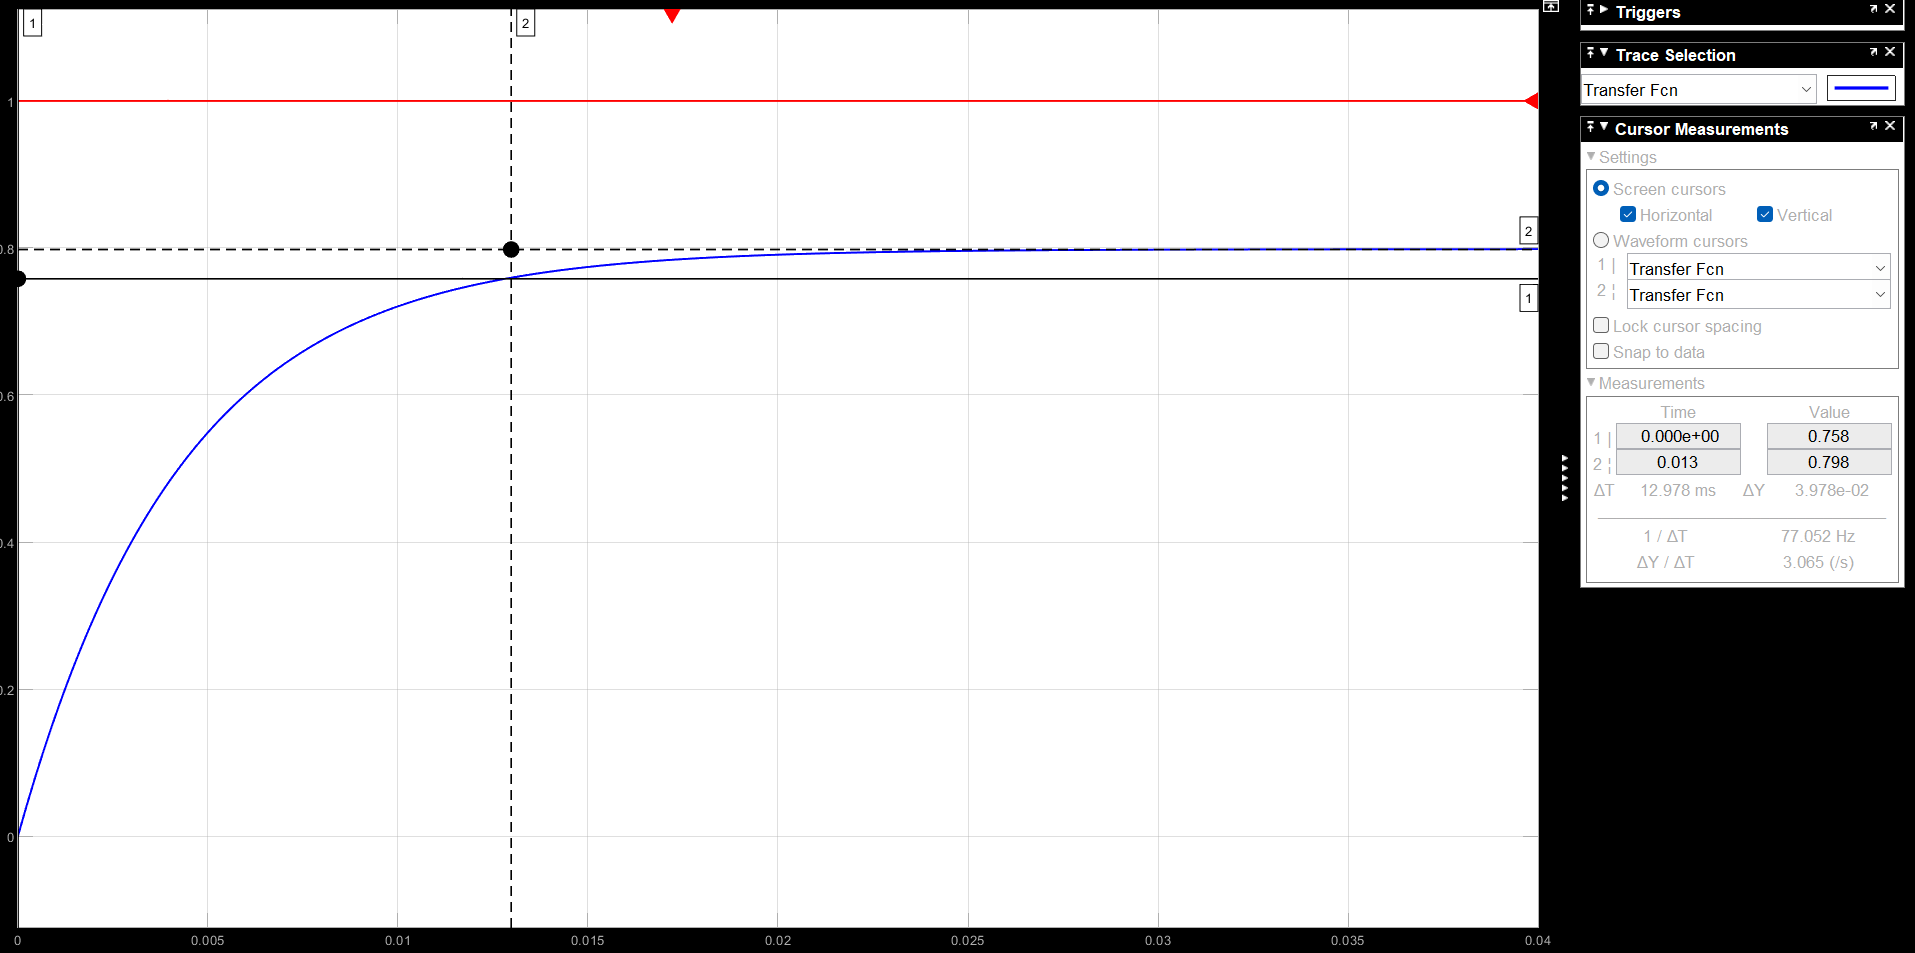
\includegraphics[width = 19 cm]{TP2 Simulink/Syst_1/tr5prct_syst_1_K=2.2.png}
\end{center}
\normalsize En utilisant la même méthode que précédemment, on mesure une erreur statique $\epsilon_s = 20.1\%$ et un temps de réponse à cinq pourcents $t_{r5\%} = 12.98$ms.
Les valeurs mesurées sont de nouveau très proches, (écart de 0.5$\%$ entre les erreurs statiques et de 1.4$\%$ entre les temps de réponse à cinq pourcents) les légers écarts sont liées à la précision de lecture du graphe.
\begin{itemize}
    \item \bf \large K = 27.2
\end{itemize}
\begin{center}
    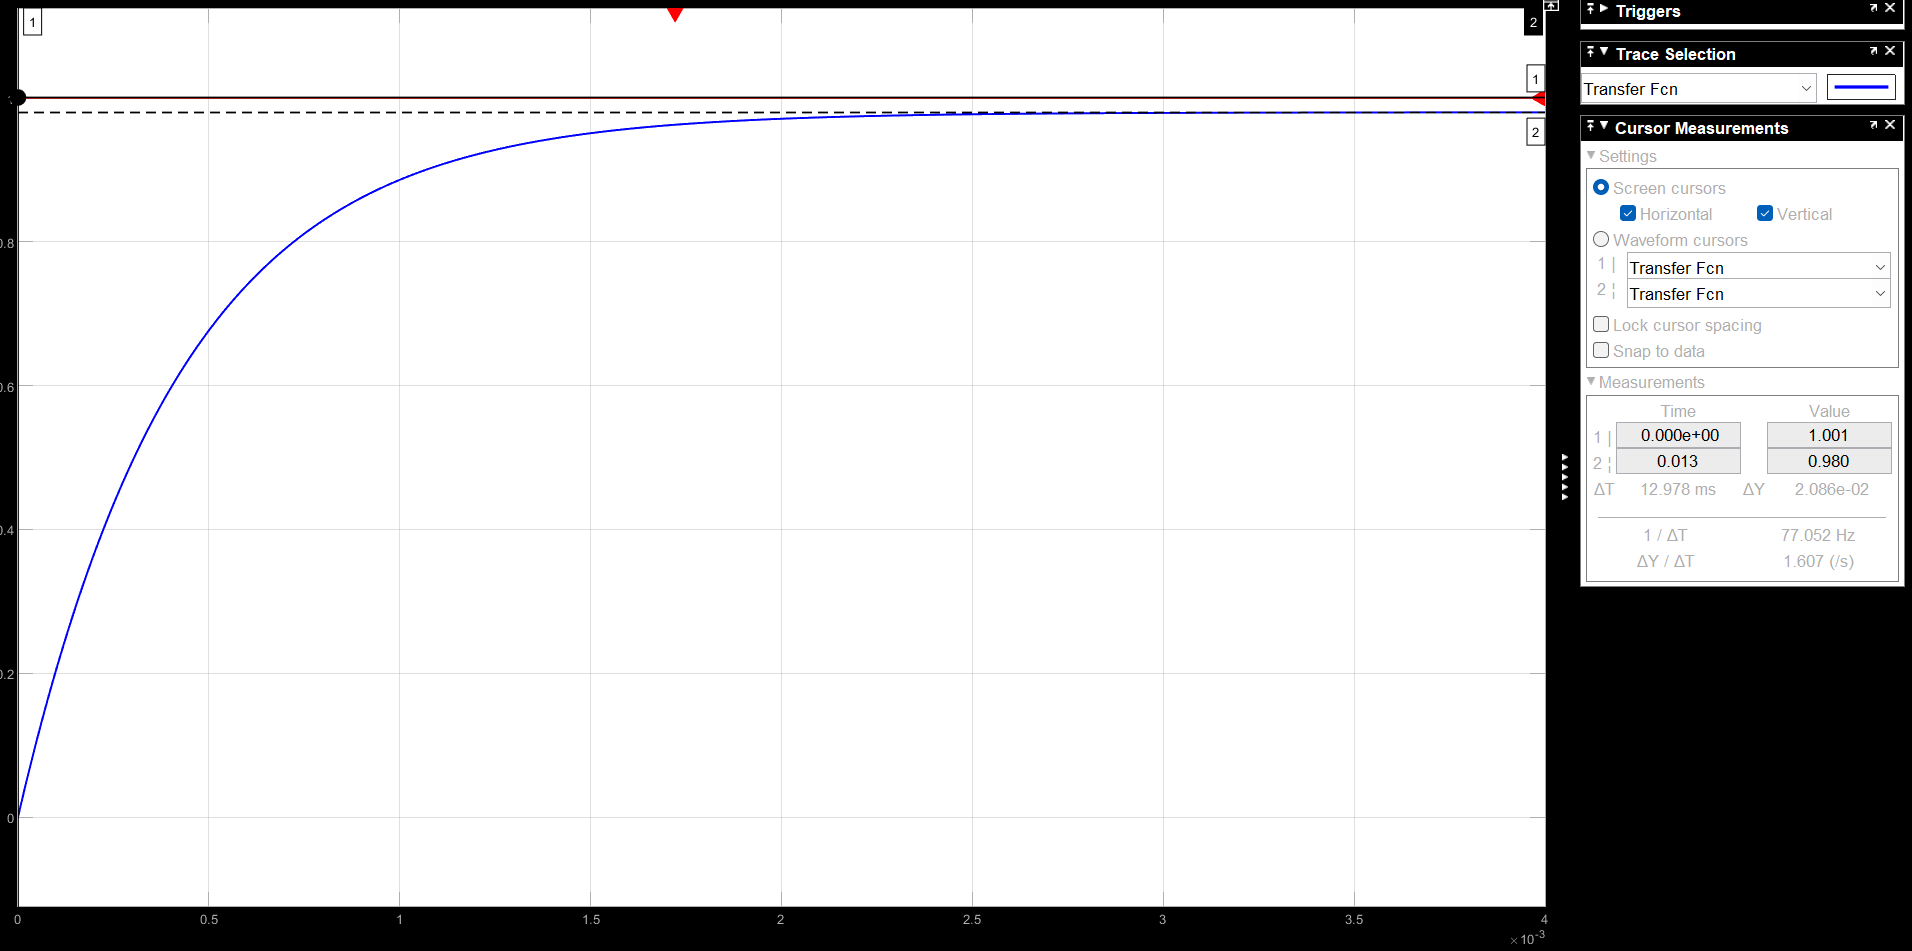
\includegraphics[width = 19 cm]{TP2 Simulink/Syst_1/err_stat_syst_1_K=27.2.png}
    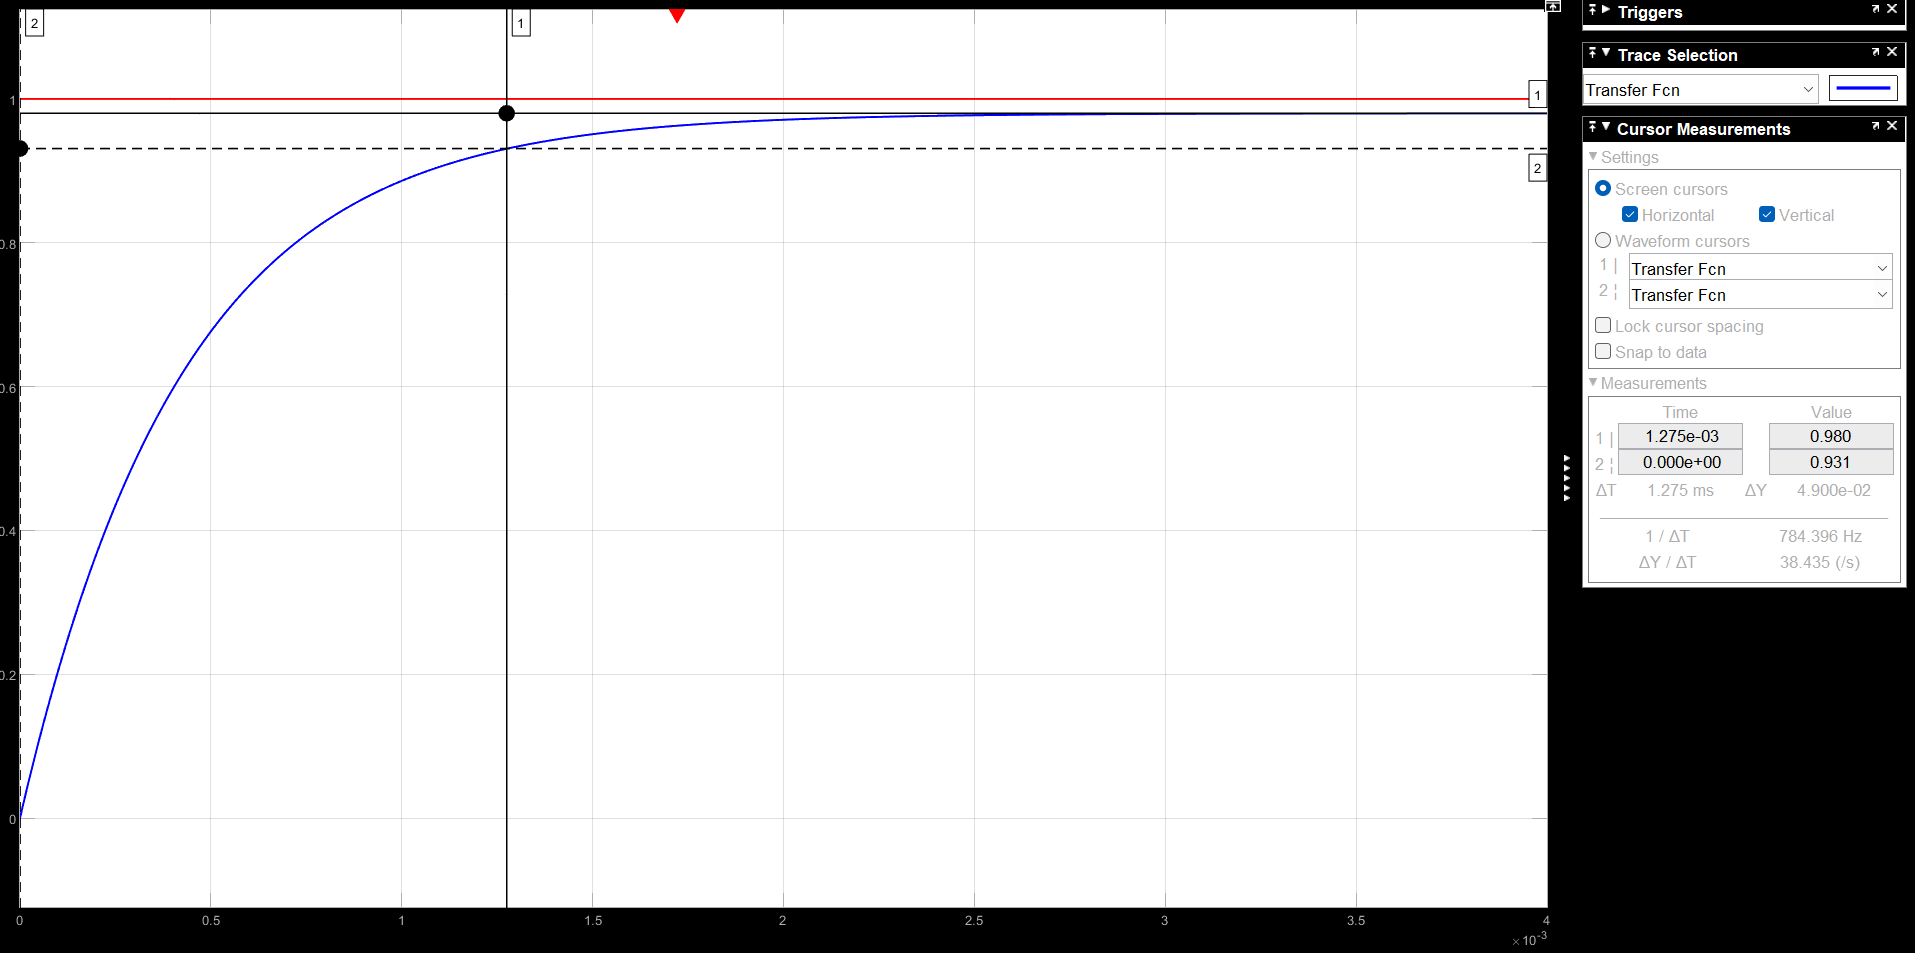
\includegraphics[width = 19 cm]{TP2 Simulink/Syst_1/tr5prct_syst_1_K=27.2.png}
\end{center}
\normalsize Enfin, pour la dernière valeur de K, on mesure une erreur statique $\epsilon_s = 2.09\%$ et un temps de réponse à cinq pourcents $t_{r5\%} = 1.27$ms.
Les valeurs mesurées sont égales pour les temps de réponse à cinq pourcents, et différentes de 4.5$\%$ pour les erreurs statiques. Cette erreur est plus élevée car le temps de réponse est très court en comparaison avec la durée de la réponse indicielle, ce qui rend difficile une lecture plus précise sur le graphe.
\newpage
Résumons toutes ces mesures dans un tableau : 
\begin{center}
    \begin{tabular}{ |p{1cm}|p{2.5cm}|p{2.5cm}|p{2.5cm}|p{2.5cm}|}

        \hline
        $K$ & \normalsize  $t_{r5\%}$(ms) th. & $t_{r5\%}$(ms) sim. & $\epsilon_s$ ($\%$) th. & $\epsilon_s$ ($\%$) sim.\\
        \hline
        4.97 & 6.39 & 6.42 & 10 & 10\\
        54.7 & 0.64 & 0.646 & 1 & 0.97\\
        2.2& 12.8 & 12.98 & 20 & 20.1\\
        27.2 & 1.27 & 1.27 & 2 & 2.09\\
        
        
        \hline
        \end{tabular}
    \end{center}
\subsubsection{\underline{\bf Correcteur intégral}}

On considère désormais un correcteur intégral $C(p) = \frac{1}{T_ip}$

\begin{itemize}
    \item Calculons la FTBF de cet asservissement : 
\end{itemize}
\begin{center}
    \large $FTBF = \frac{\frac{A}{T_ip(1+\tau p)}}{1 + \frac{A}{T_ip(1+\tau p)}} = \frac{A}{A + T_ip + T_i\tau p^2} = \frac{1}{1 + \frac{T_i}{A} + \frac{T_i \tau}{A}p^2} = \frac{A_{BF}}{1 + \frac{2z}{\omega_{BF}} + \frac{p^2}{w_{BF}^2}}$

\end{center}
\normalsize On obtient bien une FTBF de second ordre et, par identification, $A_{BF} = 1$,\fbox{$\omega_{BF} = \sqrt{\frac{A}{T_i\tau}}$}, et $\frac{2z}{w_{BF}} = \frac{T_i}{A} \Leftrightarrow $\fbox{$z = \frac{1}{2}\sqrt{\frac{T_i}{\tau A}}$}

\begin{itemize}
    \item Calculons désormais l'erreur statique : 
\end{itemize}

D'après le théorème de la valeur finale : 
$\epsilon_s = \lim_{t \to \infty}\epsilon(t) = \lim_{p \to 0}p\epsilon(p)$ or $\frac{\epsilon(p)}{E(p)} = \frac{1}{1 + \frac{1}{T_ip}\frac{A}{(1+\tau p)}}$ et $E(p) = \frac{E_0}{p}$ donc en injectant :
$\epsilon_s = \lim_{p \to 0}p \times \frac{E_0}{p}\times \frac{1}{1 + \frac{1}{T_ip}\frac{A}{(1+\tau p)}} = 0$.
\\L'erreur statique est donc nulle, ce qui est le principal avantage du correcteur intégral. Cependant, nous avons montré que la FTBF était de second ordre, et que $z = \frac{1}{2}\sqrt{\frac{T_i}{\tau A}}$. Donc plus z diminue, donc plus $T_i$ diminue, le système devient plus nerveux et moins amorti alors que si $T_i$ augmente, le système est plus amorti mais moins nerveux.
\\De plus, on cherche à calculer $T_i$ pour que la réponse indicielle en boucle fermée présente un dépassement de 5$\%$.
D'après les abaques, pour un premier dépassement à 5$\%$ : $z=0.7$ et $T_i = (2z)^2\times\tau A \Rightarrow T_i = (0.7\times2)^2\times21.3.10^{-3}\times1.81 = 0.0756$.
Ainsi, on peut déterminer $\omega_{BF} = \sqrt{\frac{A}{T_i \tau}} = 33.526$ rad/s.
\\Ensuite, d'après la deuxième abaque, pour $z=0.7$, on récupère le temps de réponse à 5$\%$ réduit :
$t_{r5\%}\omega_{BF} = 3 \Leftrightarrow t_{r5\%} = \frac{3}{\omega_{BF}} = \frac{3}{33.526} = 89$ms.
\newpage
\large \textit{ \textbf{Simulation}}
\\\normalsize Le système simulé dans Simulink est relativement le même que pour le correcteur proportionnel : 
\begin{center}
    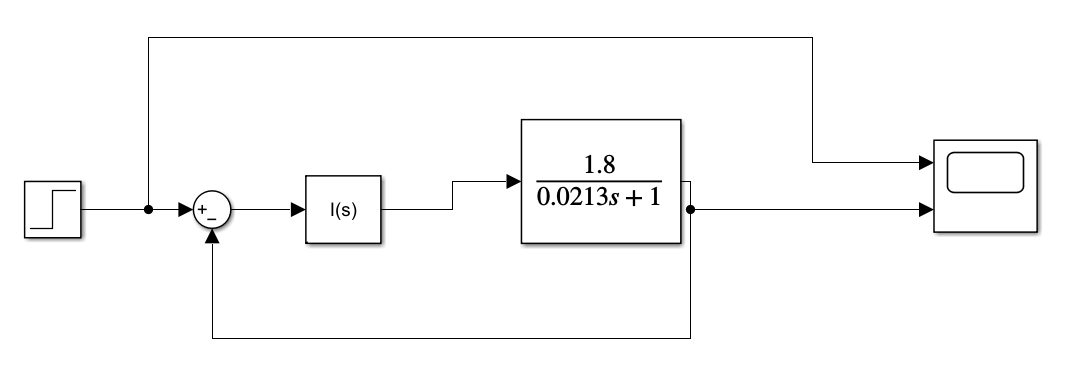
\includegraphics[width = 15 cm]{TP2 Simulink/Syst_1/Syst1_Simulink_I.png}
\end{center}

Traçons désormais les réponses indicielles pour différentes valeurs de $T_i$ : 
\begin{itemize}
    \item \large $\mathbf{T_i = \tau = 0.0213}$
\end{itemize}

\begin{center}
    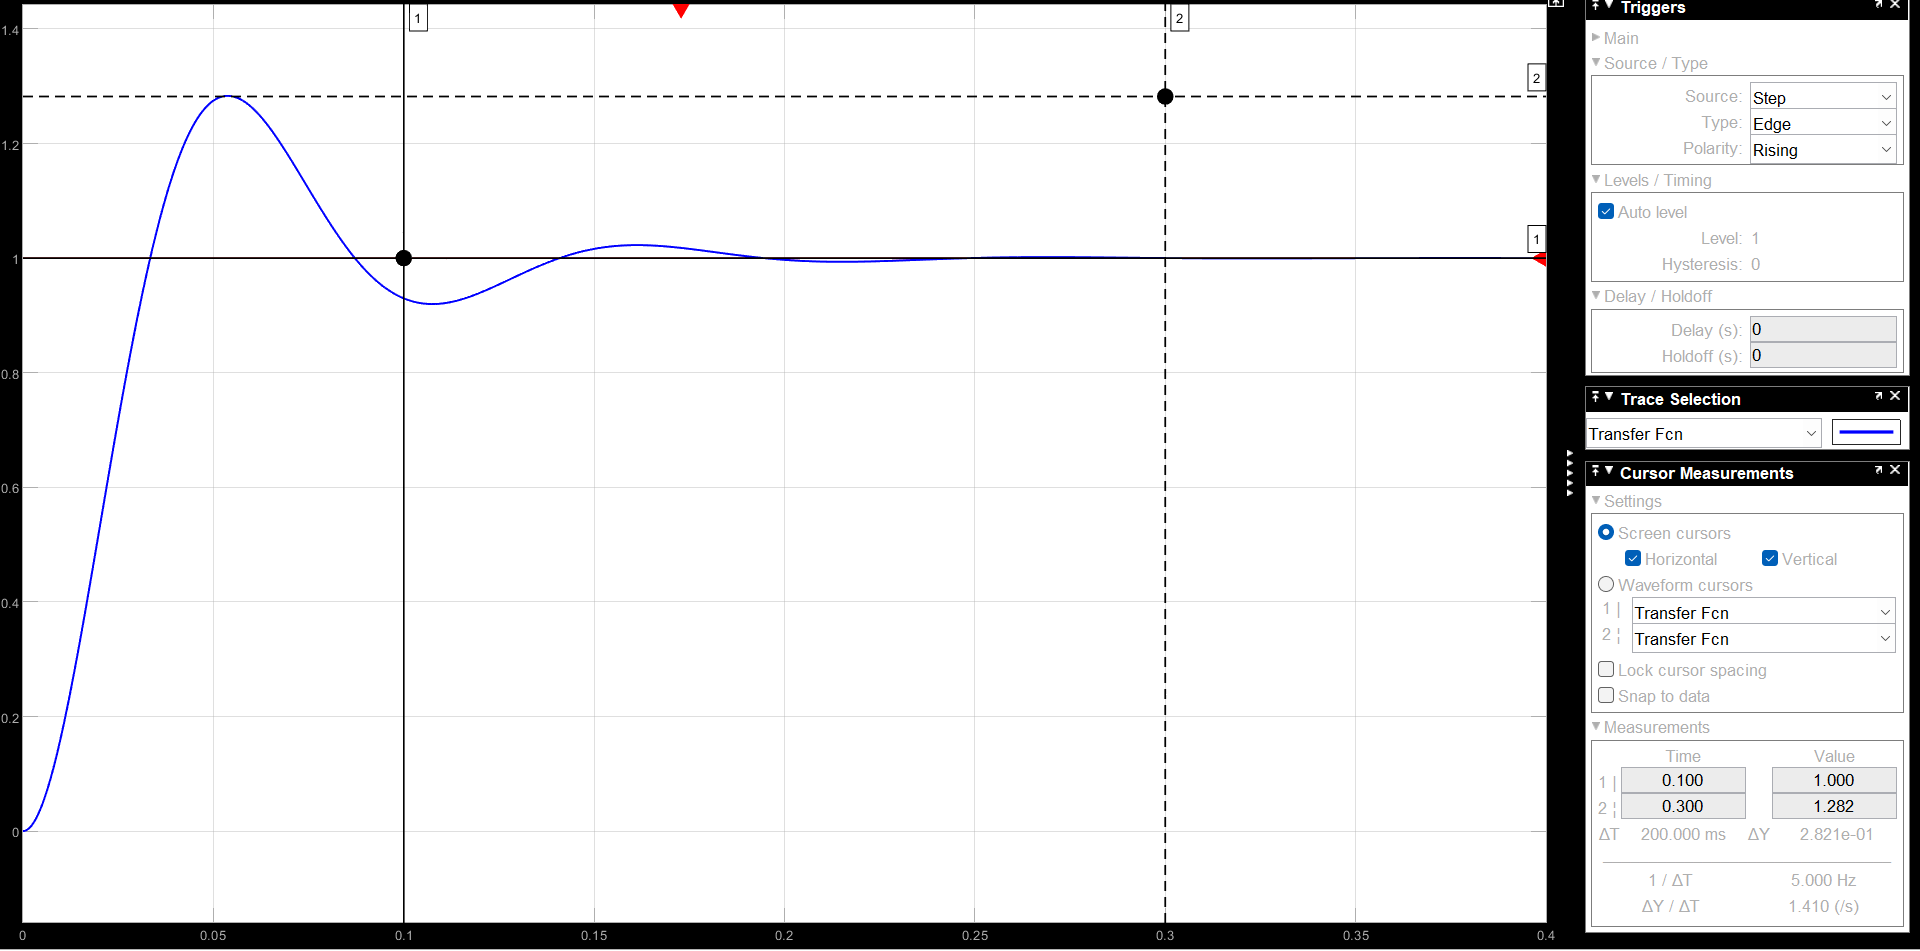
\includegraphics[width = 19 cm]{TP2 Simulink/Syst_1/depassement_syst1_Ti=tau.png}
    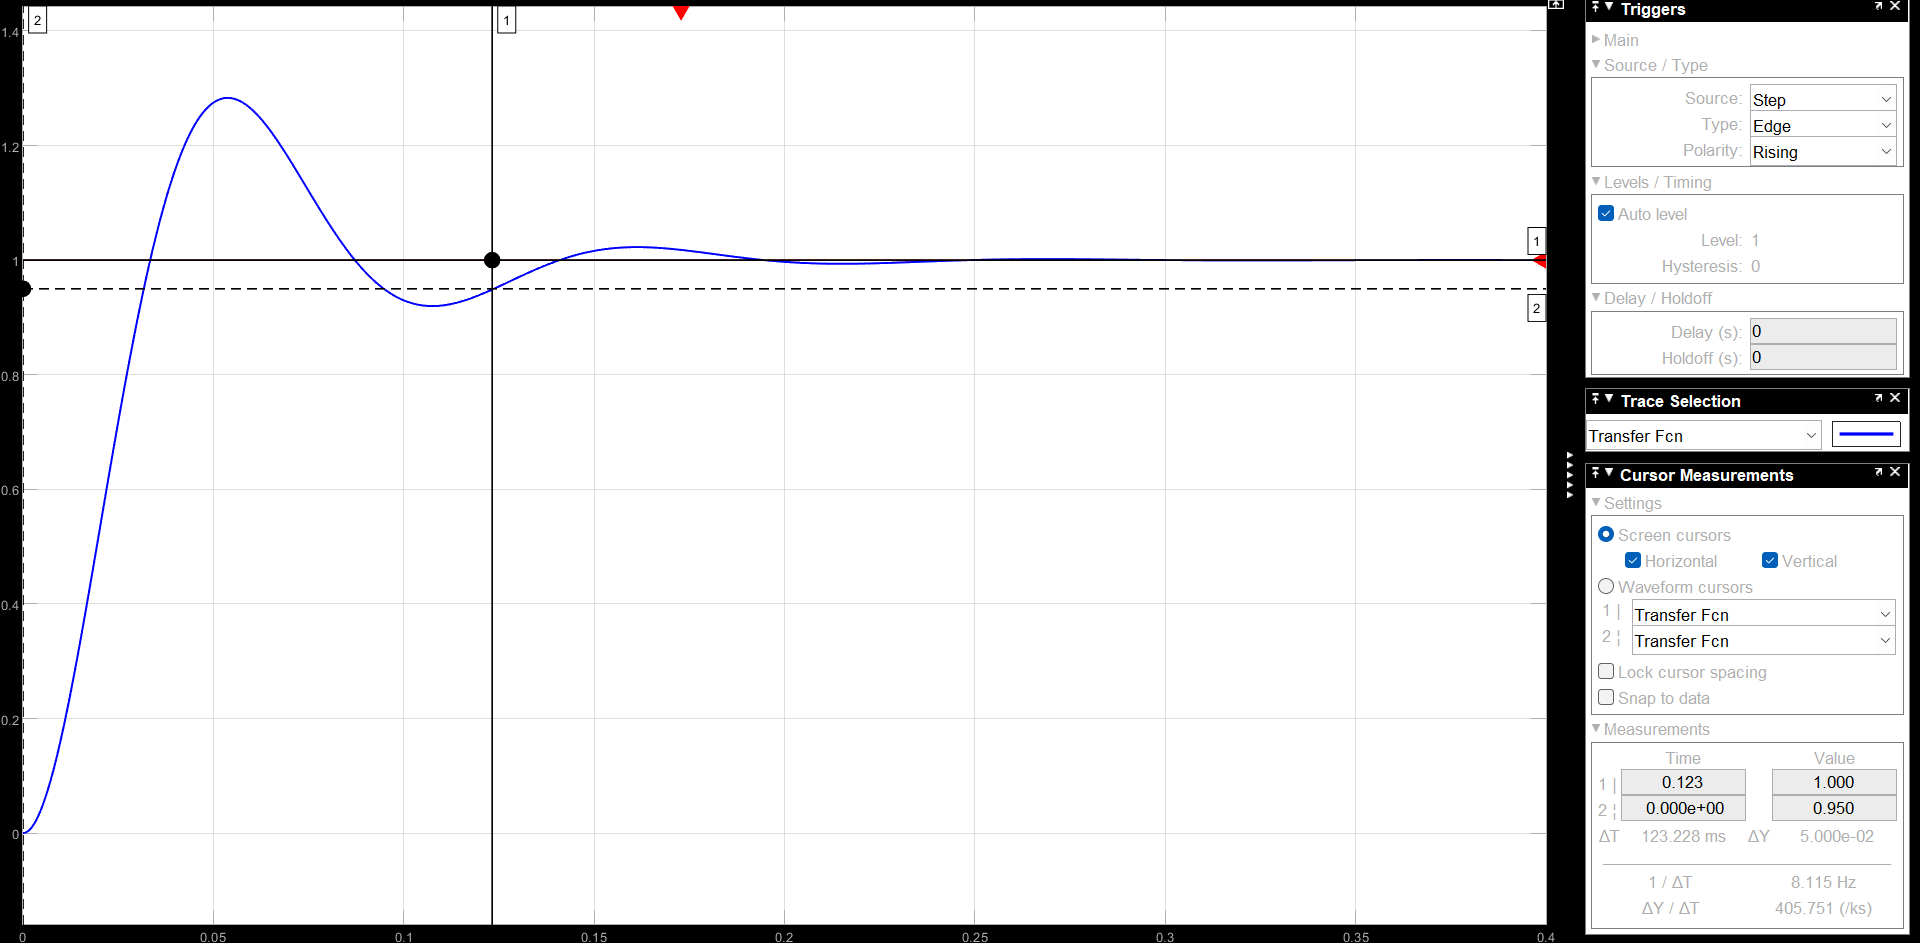
\includegraphics[width = 19 cm]{TP2 Simulink/Syst_1/tr5prct_syst_1_Ti=tau.png}
\end{center}
\normalsize Le premier graphe permet de mesurer l'amplitude du premier dépassement : la réponse atteint 1 en régime permanent et le premier dépassement atteint son maximum en 1.28. On en déduit donc que l'amplitude du premier dépassement est de 28.2$\%$.
On remarque aussi qu'on a bien une erreur statique nulle (la réponse indicielle atteint 1 en régime permanent tout comme l'échelon : $\epsilon_s = 1-1 = 0\%$).
La deuxième capture d'écran permet de lire le temps de réponse à 5$\%$. La méthode pour le mesurer est cependant différente que pour le correcteur proportionnel : la réponse présente des dépassements, il faut donc trouver le point où la réponse de dépasse plus de 5$\%$ du régime permanent ou ne passe plus en dessous de 95$\%$ du régime permanent.
Avec cette méthode, nous avons trouvé que $t_{r5\%} = 123.23$ms.
\\\\\underline{\bf Diagramme de Black de la FTBO :}
\\On rappelle que :
\begin{center}
    \large$FTBO = \frac{A}{\tau p + T_i\tau p^2}$
\end{center}
\normalsize Avec notre valeur de $T_i$, on obtient :
\begin{center}
    \large$FTBO = \frac{1.81}{0.0213p + 4.5369.10^{-4}p^2}$
\end{center}
\normalsize On peut maintenant tracer le diagramme de Black à l'aide Matlab en exécutant la fonction :
\begin{verbatim}
    T=tf([coeff num],[coeff den]) 
\end{verbatim}
Et ensuite :
\begin{verbatim}
    nichols(T)
\end{verbatim}
On obtient alors : 
\begin{center}
    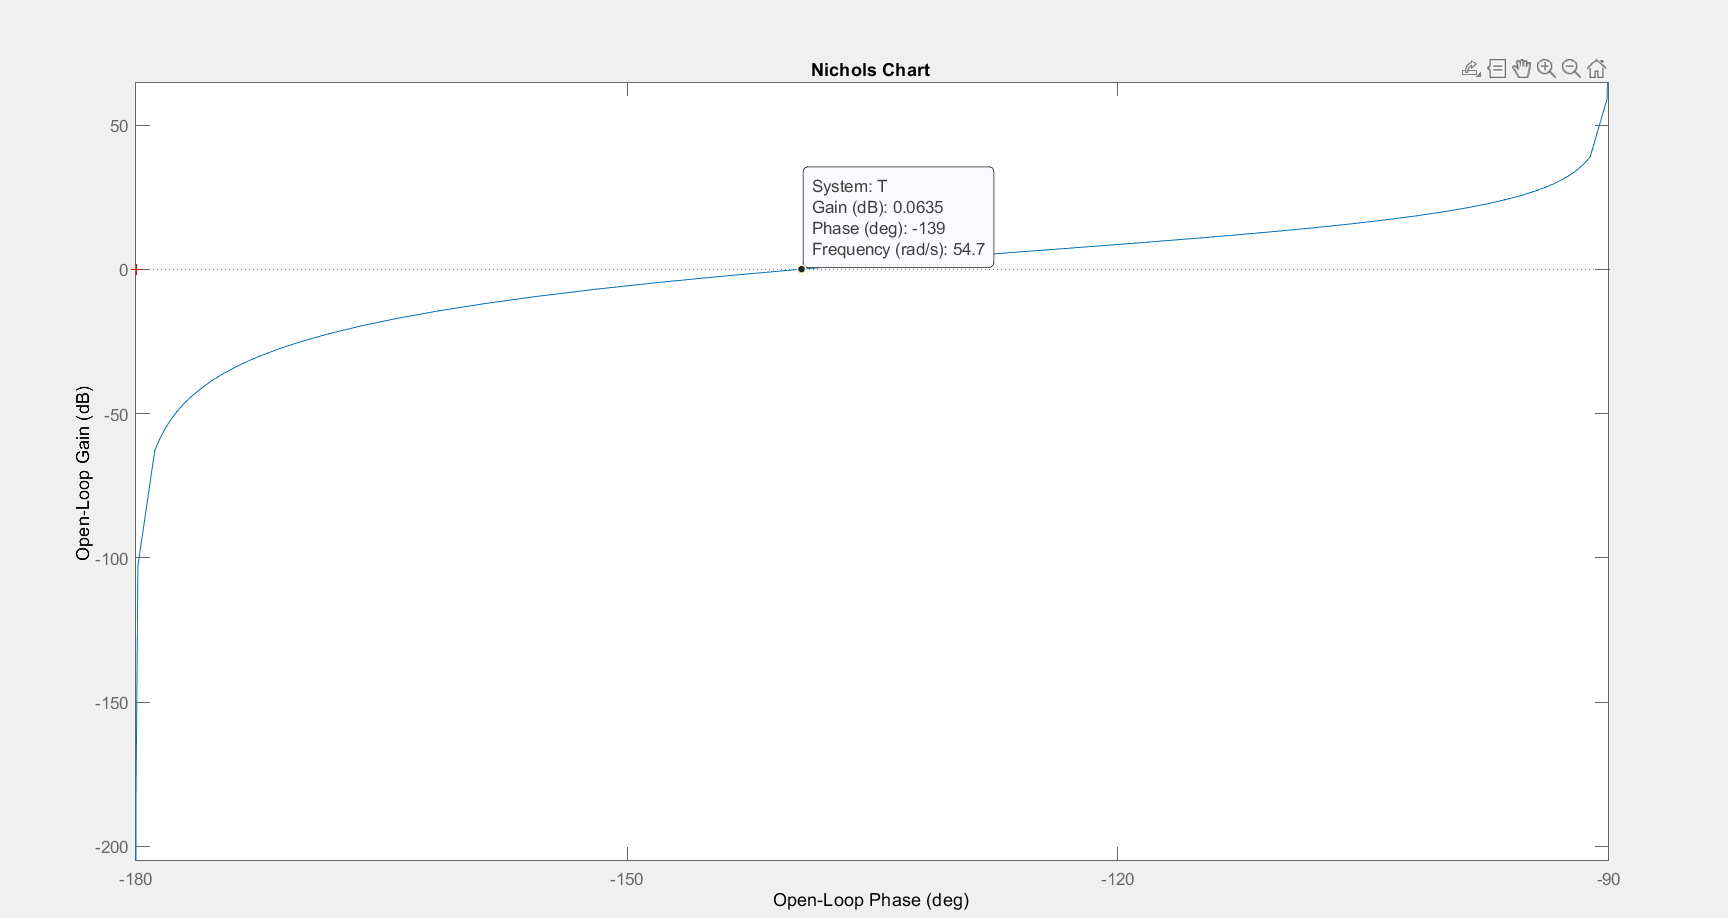
\includegraphics[width = 19 cm]{TP2 Simulink/Syst_1/Ti=tau_syst_1_Black.png}
\end{center}
Pour calculer la marge de phase, il faut récupérer l'abscisse du point où la courbe coupe l'axe $y=0$ et faire la différence entre cette abscisse et $-180$.
\\Ainsi on trouve comme marge de phase \fbox{$m_{\phi_{\tau}} = -139-(-180) = 41^{\circ}$}.
\newpage
\begin{itemize}
    \item \large $\mathbf{T_i = 5\tau = 0.1065}$
\end{itemize}
\begin{center}
    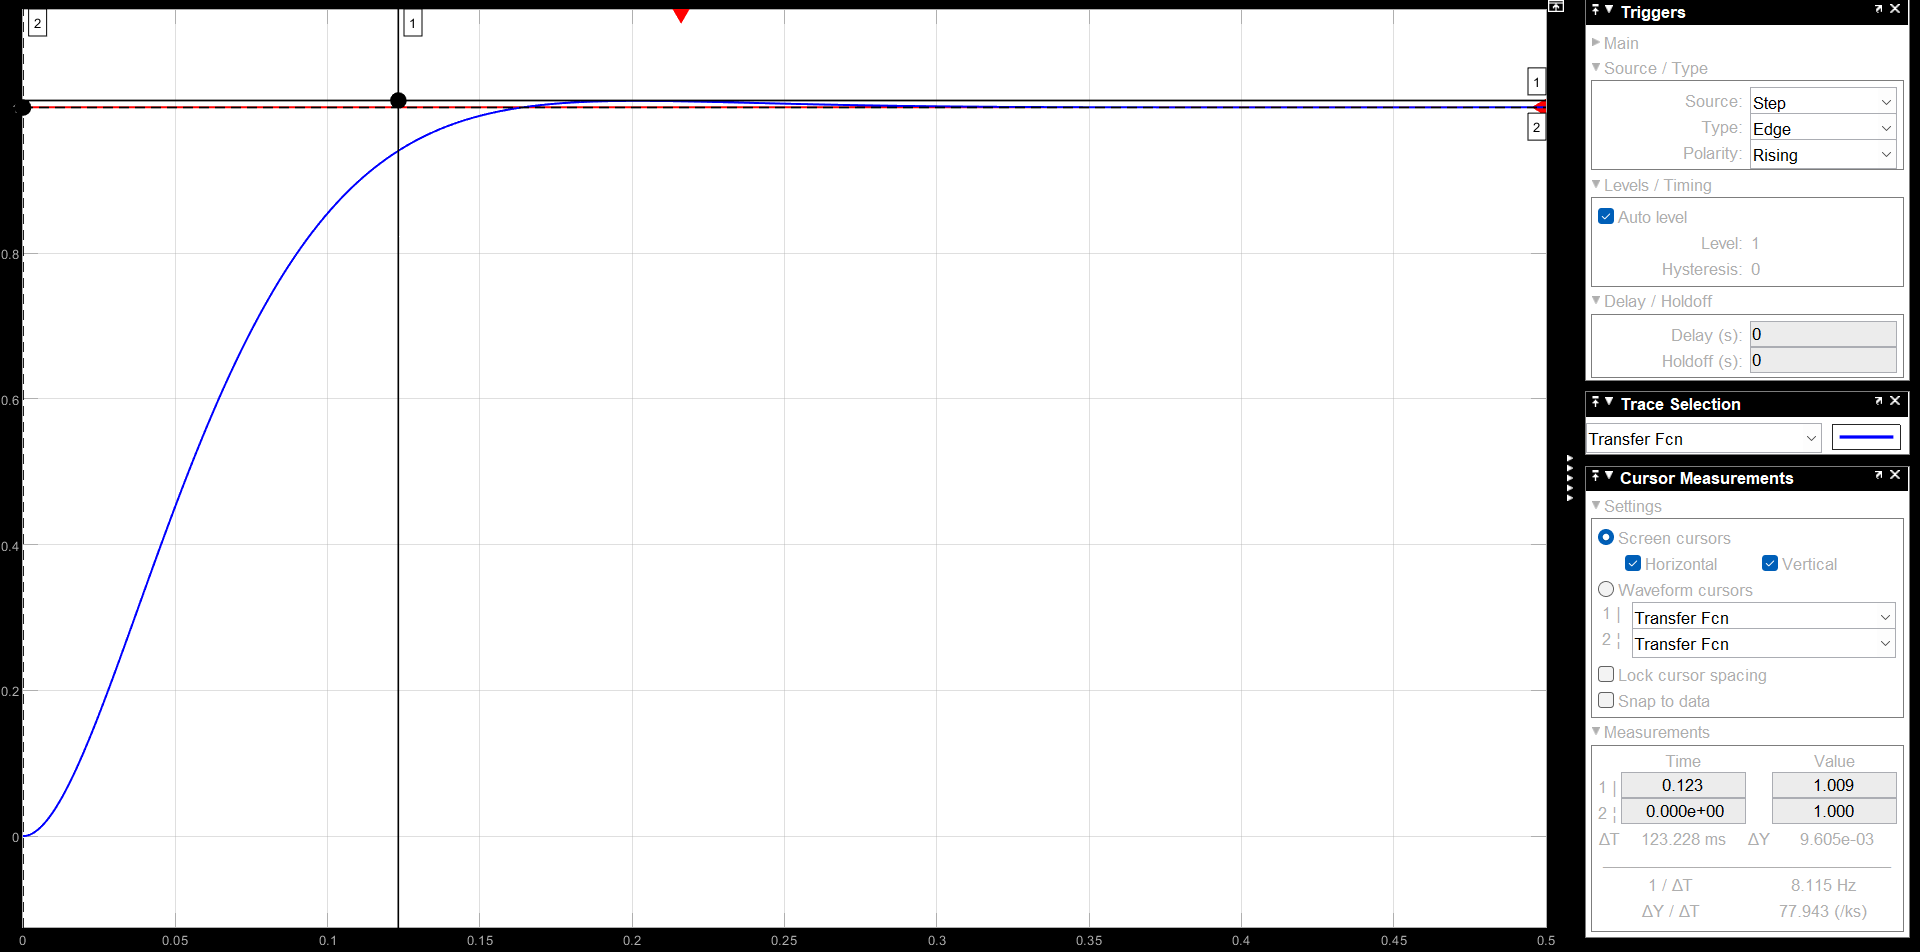
\includegraphics[width = 19 cm]{TP2 Simulink/Syst_1/depassement_syst_1_Ti=5tau.png}
    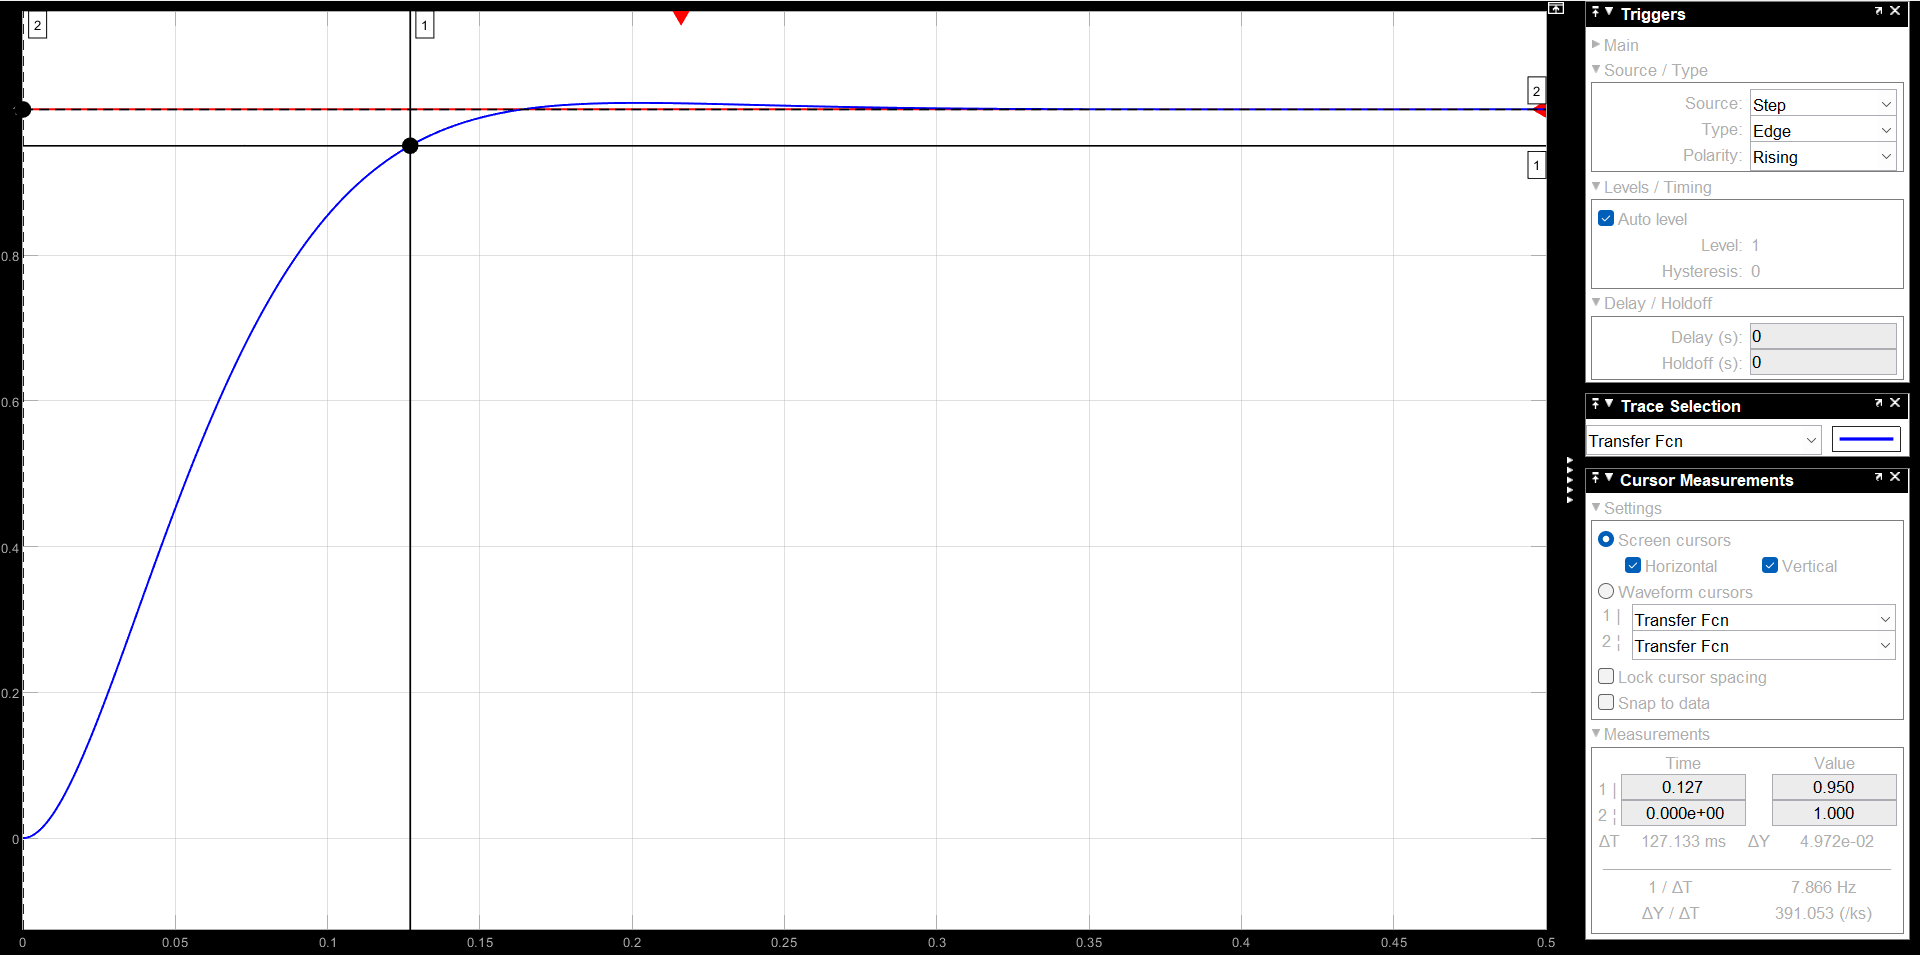
\includegraphics[width = 19 cm]{TP2 Simulink/Syst_1/tr5prct_syst_1_Ti=5tau.png}
    
\end{center}
\normalsize Le premier graphe permet de mesurer l'amplitude du premier dépassement : la réponse atteint 1 en régime permanent et le premier dépassement atteint son maximum en 1.01. On en déduit donc que l'amplitude du premier dépassement est de 1$\%$.
On remarque aussi qu'on a bien une erreur statique nulle (la réponse indicielle atteint 1 en régime permanent tout comme l'échelon : $\epsilon_s = 1-1 = 0\%$).
La deuxième capture d'écran permet de lire le temps de réponse à 5$\%$ : $t_{r5\%} = 127.1$ms
\\\\\underline{\bf Diagramme de Black de la FTBO :}
\\\normalsize Avec notre valeur de $T_i = 5\tau$, on a :
\begin{center}
    \large$FTBO = \frac{1.81}{0.1065p + 2.26.10^{-2}p^2}$
\end{center}
\normalsize On peut maintenant tracer le diagramme de Black à l'aide Matlab :
\begin{center}
    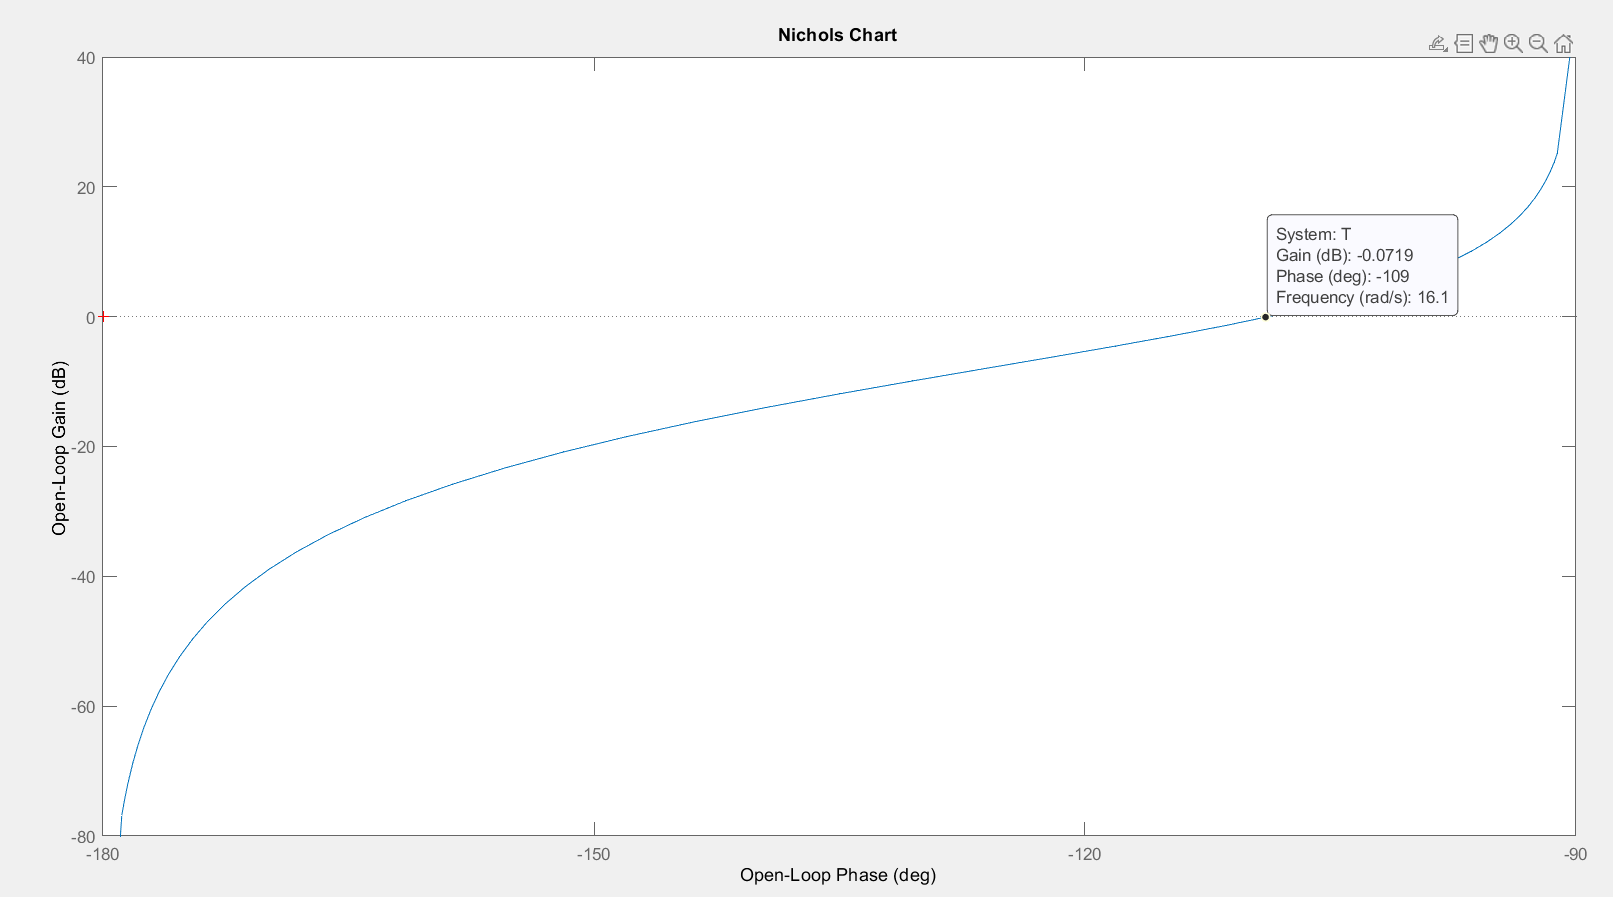
\includegraphics[width = 19 cm]{TP2 Simulink/Syst_1/Ti=5tau_syst_1_Black.png}
\end{center}
Pour calculer la marge de phase, il faut récupérer l'abscisse du point où la courbe coupe l'axe $y=0$ et faire la différence entre cette abscisse et $-180$.
\\Ainsi on trouve comme marge de phase \fbox{$m_{\phi_{5\tau}} = -109-(-180) = 71^{\circ}$}.
\newpage
\begin{itemize}
    \item \large $\mathbf{T_i = 10\tau = 0.213}$
\end{itemize}
\begin{center}
    
    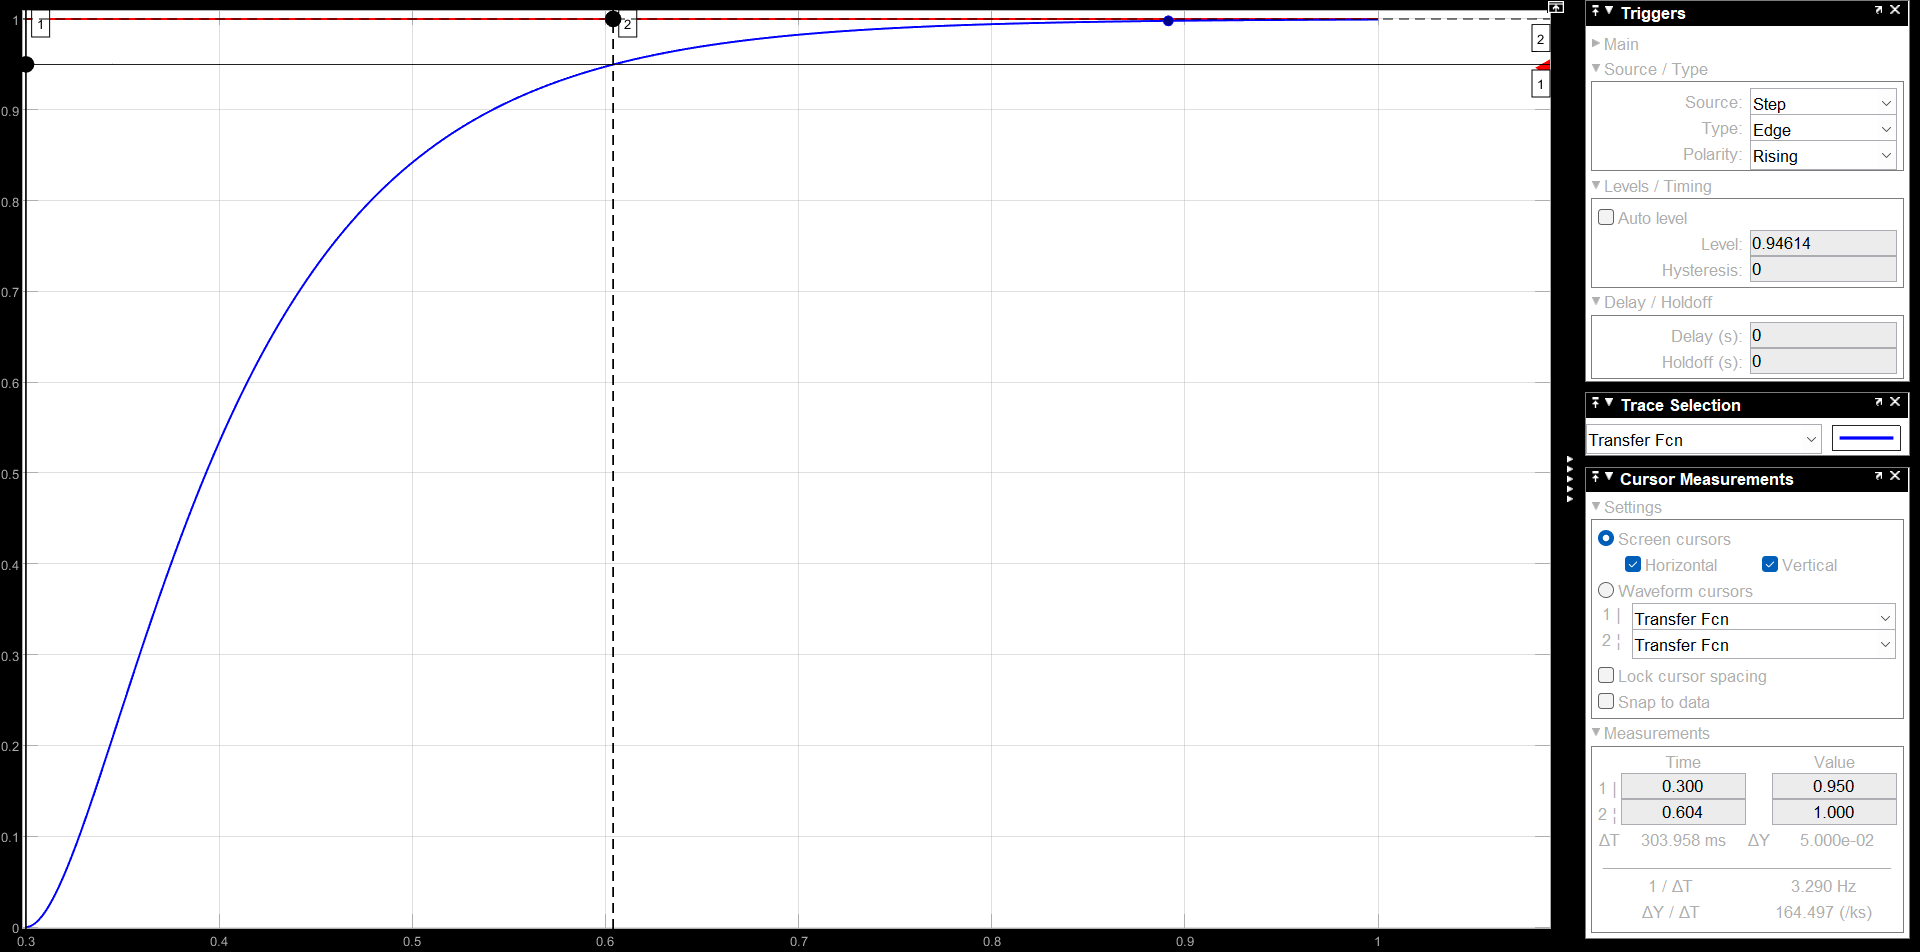
\includegraphics[width = 19 cm]{TP2 Simulink/Syst_1/tr5prct_syst1_Ti=10tau.png}
    
\end{center}
\normalsize Le premier graphe permet de mesurer l'amplitude du premier dépassement : la réponse atteint 1 en régime permanent et le premier dépassement atteint son maximum en 1.01. On en déduit donc que l'amplitude du premier dépassement est de 1$\%$.
On remarque aussi qu'on a bien une erreur statique nulle (la réponse indicielle atteint 1 en régime permanent tout comme l'échelon : $\epsilon_s = 1-1 = 0\%$).
La deuxième capture d'écran permet de lire le temps de réponse à 5$\%$ : $t_{r5\%} = 304$ms
\\\\\underline{\bf Diagramme de Black de la FTBO :}
\\\normalsize Avec notre valeur de $T_i = 10\tau$, on a :
\begin{center}
    \large$FTBO = \frac{1.81}{0.213p + 4.5369.10^{-3}p^2}$
\end{center}
\normalsize On peut maintenant tracer le diagramme de Black à l'aide Matlab :
\begin{center}
    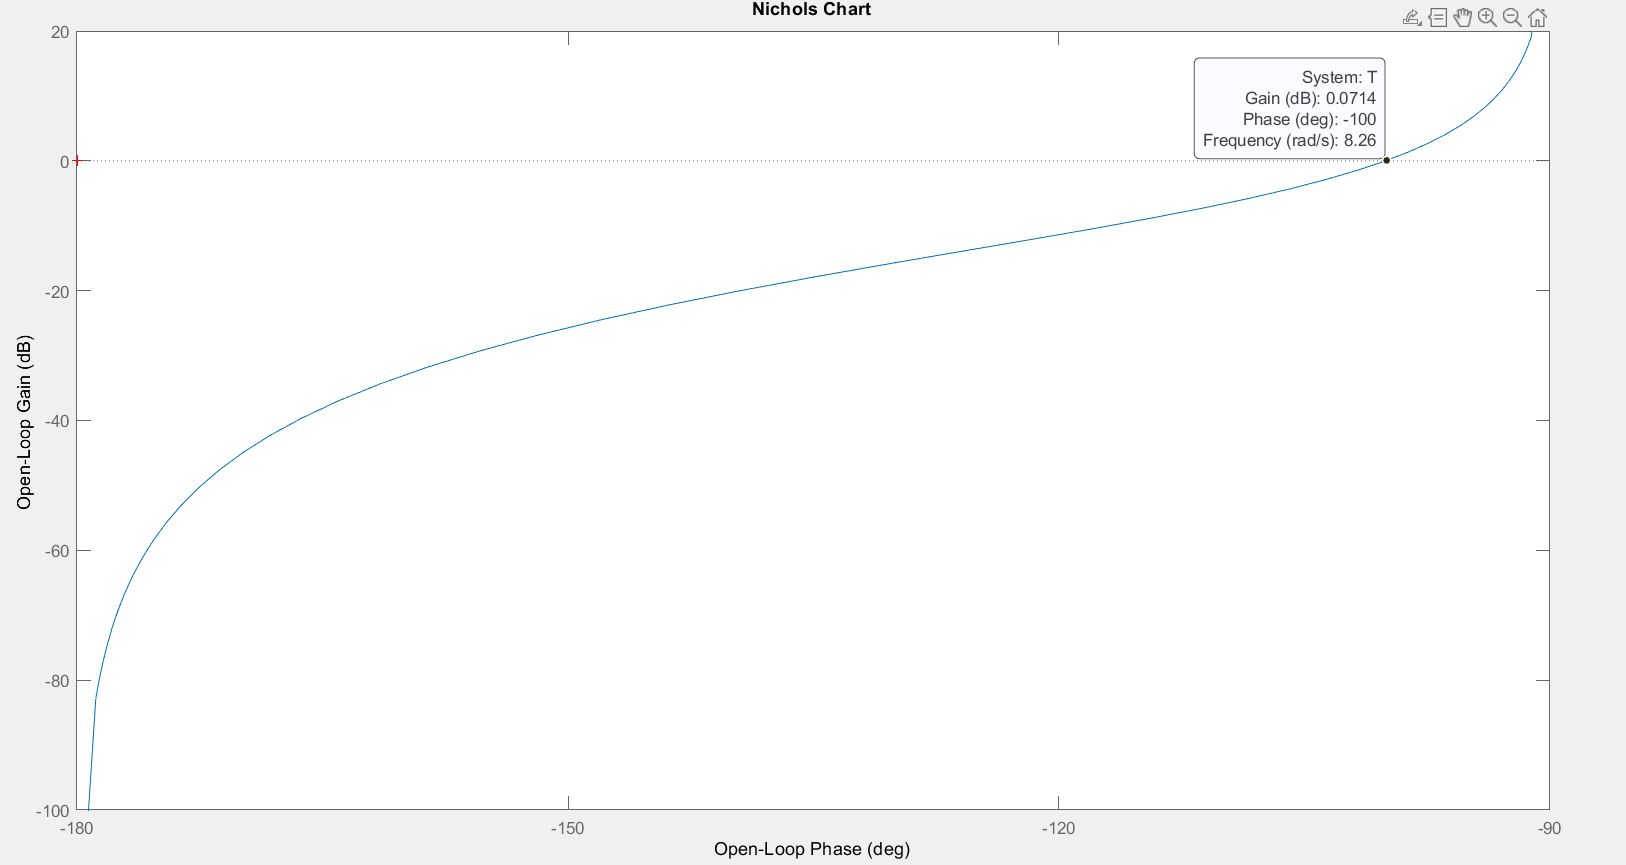
\includegraphics[width = 19 cm]{TP2 Simulink/Syst_1/Ti=10tau_syst_1_Black.png}
\end{center}
On en déduit ainsi la marge de phase :\fbox{$m_{\phi_{10\tau}} = -100-(-180) = 80^{\circ}$}.
\\\\\underline{\bf Conclusion :} Les résultats obtenus sont bien cohérents : on a bien une baisse de nervosité et une hausse d'amortissement quand $T_i$ augmente.
En effet, pour $T_i = \tau$ et $T_i = 5\tau$, la réponse indicielle présentait des dépassements, mais plus aucun pour $T_i = 10\tau$. On peut aussi remarquer que les temps de réponse à 5$\%$ augmentent aussi quand $T_i$ augmente, ce qui confirme que si $T_i$ augmente, le système est plus lent.
\\Enfin, la marge de phase nous permet de nous assurer de la stabilité des systèmes : d'après le \textbf{critère géométrique du revers} dans le plan de Black on sait que le système est stable en boucle fermée si et seulement si le lieu de Black de la fonction de transfert en boucle ouverte, parcouru dans le sens des pulsations croissantes, laisse le point (-180$^{\circ}$,0\textit{dB}) à sa droite.
Or dans notre cas, nous avons bien tracé le lieu de Black de la FTBO et, pour chaque valeur de $T_i$, le point critique est à la droite du lieu de Black.
De plus on peut aussi dire que comme toutes les marges de phase mesurées sont positives, les systèmes sont stables. Mais on peut aussi quatifier l'éloignement du système de l'instabilité : plus la marge de phase est grande (et positive), plus le système est stable. Dans notre cas, on avait :
\\Pour $T_i = \tau$, $\mathbf{m_{\phi_{\tau}} = 41^{\circ}}$  ; $T_i = 5\tau$, $\mathbf{m_{\phi_{5\tau}} = 71^{\circ}}$ et $T_i = 10\tau$, $\mathbf{m_{\phi_{10\tau}} = 80^{\circ}}$.
On a bien un système qui devient de plus en plus stable quand $T_i$ augmente.
\\\\Traçons désormais la réponse indicielle avec la valeur de $T_i$ pour laquelle elle présente un dépassement de 5$\%$ : 
\begin{center}
    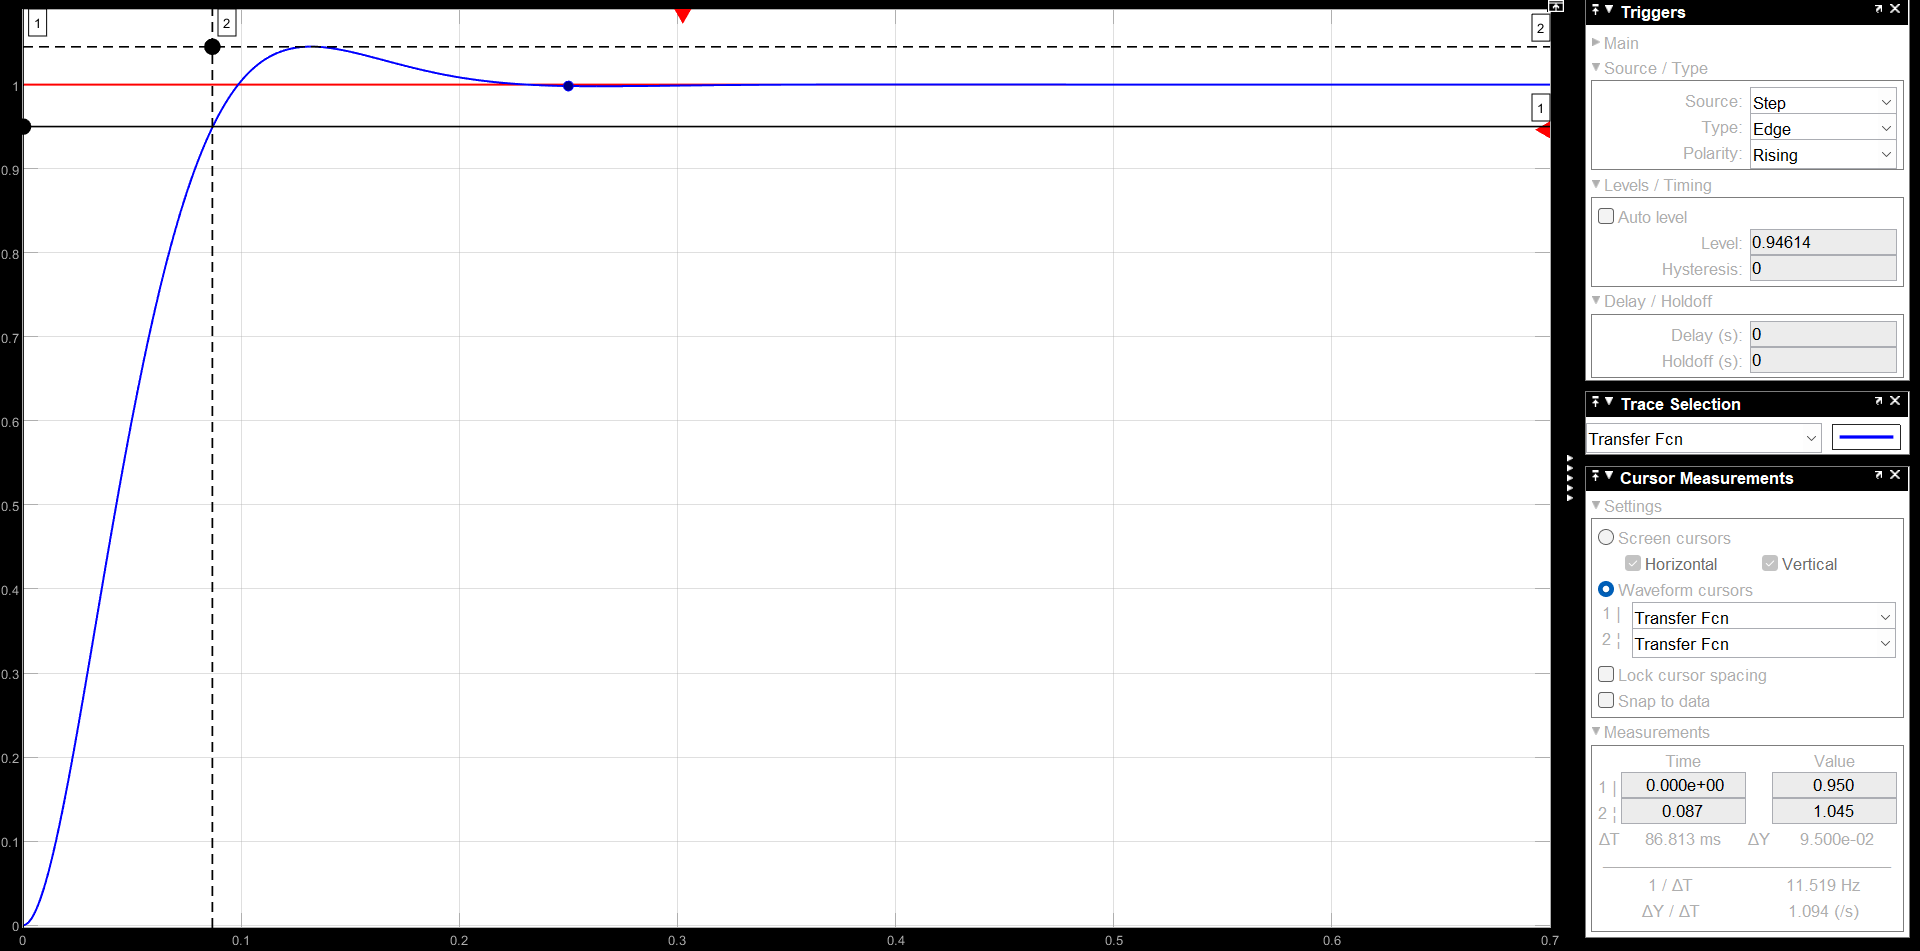
\includegraphics[width = 19 cm]{TP2 Simulink/Syst_1/dep5prct_syst1.png}
\end{center}

On peut lire sur cette capture d'écran à la fois le temps de réponse à 5$\%$ et l'amplitude du premier dépassement. L'échelon atteint 1, tout comme la réponse indicielle donc l'erreur statique est nulle et le premier dépassement atteint 1.045, donc le premier dépassement dépasse de 4.5$\%$ le régime permanent. Le temps de réponse à 5$\%$ de ce système est de 86,8 ms.
En comparaison, on attendait : $D_1 = 5\%$ et $t_{r5\%} = 89$ms. Cet écart peut s'expliquer par une mauvaise précision de lecture sur les abaques lors du calcul de $T_i$ pour avoir un premier dépassement à 5$\%$.
\\\\\underline{\bf Conclusion :} Pour résumer, d'après toutes les simulations et calculs théoriques, on se rend compte que pour un correcteur proportionnel, plus sa valeur augmente, plus son erreur statique et son temps de réponse diminuent sans présenter de dépassement, alors que pour le correcteur intégral, son erreur statique est toujours nulle mais la FTBO du sytème devient un deuxième ordre donc la réponse indicielle contient des dépassement qui diminuent en amplitude si $T_i$ augmente mais alors le temps de réponse devient très grand (0.3 secondes pour $T_i = 10\tau$). Pour ce système, le correcteur proportionnel est meilleur que le correcteur intégral sans compter l'erreur statique (mais qui tend vers 0 lorsque K augmente). 
\newpage
\subsection{\itshape Système 2}
\subsubsection{\underline{\itshape \bf Correcteur proportionnel}}
On considère dans un premier temps un correcteur proportionnel $C(p) = K > 0$ et le système 2 qui est modélisé par une fonction de transfert du deuxième ordre $T(s) = F_2(s) = \frac{A}{1 + 2z\frac{p}{\omega_0} + (\frac{p}{\omega_0})^2}$.
\begin{itemize}
    \item Calculons la Fonction de Transfert en Boucle Fermée (FTBF) grâce à la formule de Black : 
\end{itemize}

\large $FTBF = \frac{K\times \frac{A}{1 + 2z\frac{p}{\omega_0} + (\frac{p}{\omega_0})^2}}{1 + K\times \frac{A}{1 + 2z\frac{p}{\omega_0} + (\frac{p}{\omega_0})^2}} = \frac{KA}{1 + 2z\frac{p}{\omega_0} + (\frac{p}{\omega_0})^2 + KA} = \frac{\frac{KA}{1 + KA}}{1 + \frac{2zp}{\omega_0(1+KA)}p + (\frac{p}{\omega_0\sqrt{1+KA}})^2} = \frac{K_{BF}}{1 + \frac{2z_{BF}p}{\omega_{0_{BF}}}+ (\frac{p}{\omega_{0_{BF}}})^2}$
\\\\\normalsize Donc \large \fbox{$K_{BF} = \frac{KA}{1 + KA}$}, \fbox{$\omega_{0_{BF}} = \omega_0\sqrt{1 + KA}$} \normalsize et \large \fbox{$z_{BF} = \frac{z}{\sqrt{1 + KA}}$}.
\\\\ \normalsize Ainsi, on peut en déduire que si K augmente, z diminue et le système devient plus nerveux, et l'erreur statique diminue. Cependant, pour un système du deuxième ordre, la phase ne dépasse pas -180$^{\circ}$ donc le système ne peut pas devenir instable. Plus K augmente, plus le système est oscillatoire, car on se rapproche de l'instabilité, mais sans jamais l'atteindre. Cependant, dans notre cas, il se peut que le modèle soit mauvais et que le système puisse devenir instable.

\begin{itemize}
    \item Calculons K pour que le système admette une erreur statique de 10$\%$ : 
\end{itemize}
La méthode est identique à celle appliquée pour le système 1. En effet, l'erreur statique concerne le régime permanent et est donc indépendante des pôles (qui régissent le régime transitoire) et la FTBF du système 1 et celle du système 2 ont la même amplification statique.
On cherche donc : 
\begin{center}
    $\epsilon_s = \frac{E_0}{10} = \frac{E_0}{1 + KA} \Leftrightarrow 1 + KA = 10 \Leftrightarrow$\fbox{$K = 4.5$} avec $A = 2$.
\end{center}
On peut ainsi en déduire $z_{BF} = \frac{z}{\sqrt{1 + KA}} = \frac{0.5}{\sqrt{10}} \approx 0.158$. D'après les abaques, le premier dépassement sera de \fbox{$D_1 = 60\%$}.
De plus, $\omega_{0_{BF}} = \omega_0\sqrt{1 + KA} = 44.6\sqrt{10} = 141.037$ rad.s$^{-1}$
D'après les abaques, le temps de réponse réduit est : $t_{r5\%}\omega_{0_{BF}} = 20 \Leftrightarrow $\fbox{$t_{r5\%} = 141.8$ ms}.

\begin{itemize}
    \item Calculons K pour que le système admette une erreur statique de 2$\%$ : 
\end{itemize}
De même : 
\begin{center}
    $\epsilon_s = \frac{2E_0}{100} = \frac{E_0}{1 + KA} \Leftrightarrow 1 + KA = 50 \Leftrightarrow$\fbox{$K = 24.5$} 
\end{center}
On peut ainsi en déduire $z_{BF} = \frac{z}{\sqrt{1 + KA}} = \frac{0.5}{\sqrt{50}} \approx 0.07$. D'après les abaques, le premier dépassement sera de \fbox{$D_1 = 80\%$}.
De plus, $\omega_{0_{BF}} = \omega_0\sqrt{1 + KA} = 44.6\sqrt{50} = 315.37$ rad.s$^{-1}$
D'après les abaques, le temps de réponse réduit est : $t_{r5\%}\omega_{0_{BF}} = 40 \Leftrightarrow $\fbox{$t_{r5\%} = 126.8$ ms}.
\newpage
\normalsize Résumons ainsi ces calculs sous forme de tableau : 

\begin{center}
    \begin{tabular}{ |p{3cm}|p{3cm}|p{3cm}|p{3cm}|}

        \hline
        $K$ & $t_{r5\%}$(ms) & $\epsilon_s$ ($\%$)&$D_1$($\%$)\\
        \hline
        4.5 & 141.8$\times 10^{-3}$ & 10 & 60\\
        24.5 & 126.8$\times10^{-3}$ & 2 & 80\\ 
        
        \hline
        \end{tabular}
    \end{center}
\large \textit{ \textbf{Simulation}}
\\\\\normalsize Dans cette partie, nous avons utilisé le logiciel "Simulink" pour tracer la réponse indicielle de
l’asservissement pour les deux valeurs de K calculées précédemment. Nous avons utilisé ce système
pour les différentes simulations : 
\begin{center}
    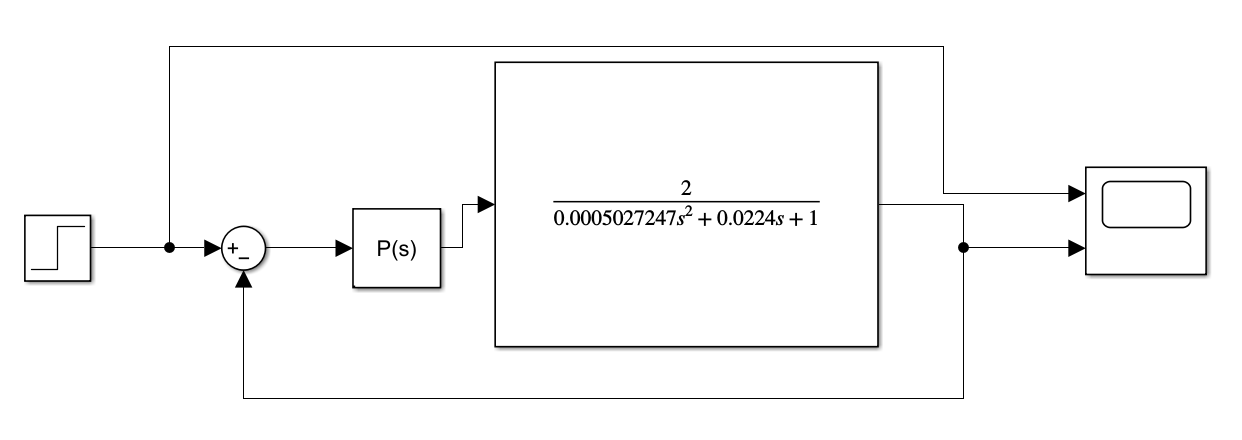
\includegraphics[width = 15 cm]{TP2 Simulink/Syst_2/Syst_2_Simunlink_P.png}
\end{center}
\begin{itemize}
    \item \bf \large K = 4.5
\end{itemize}
\begin{center}
    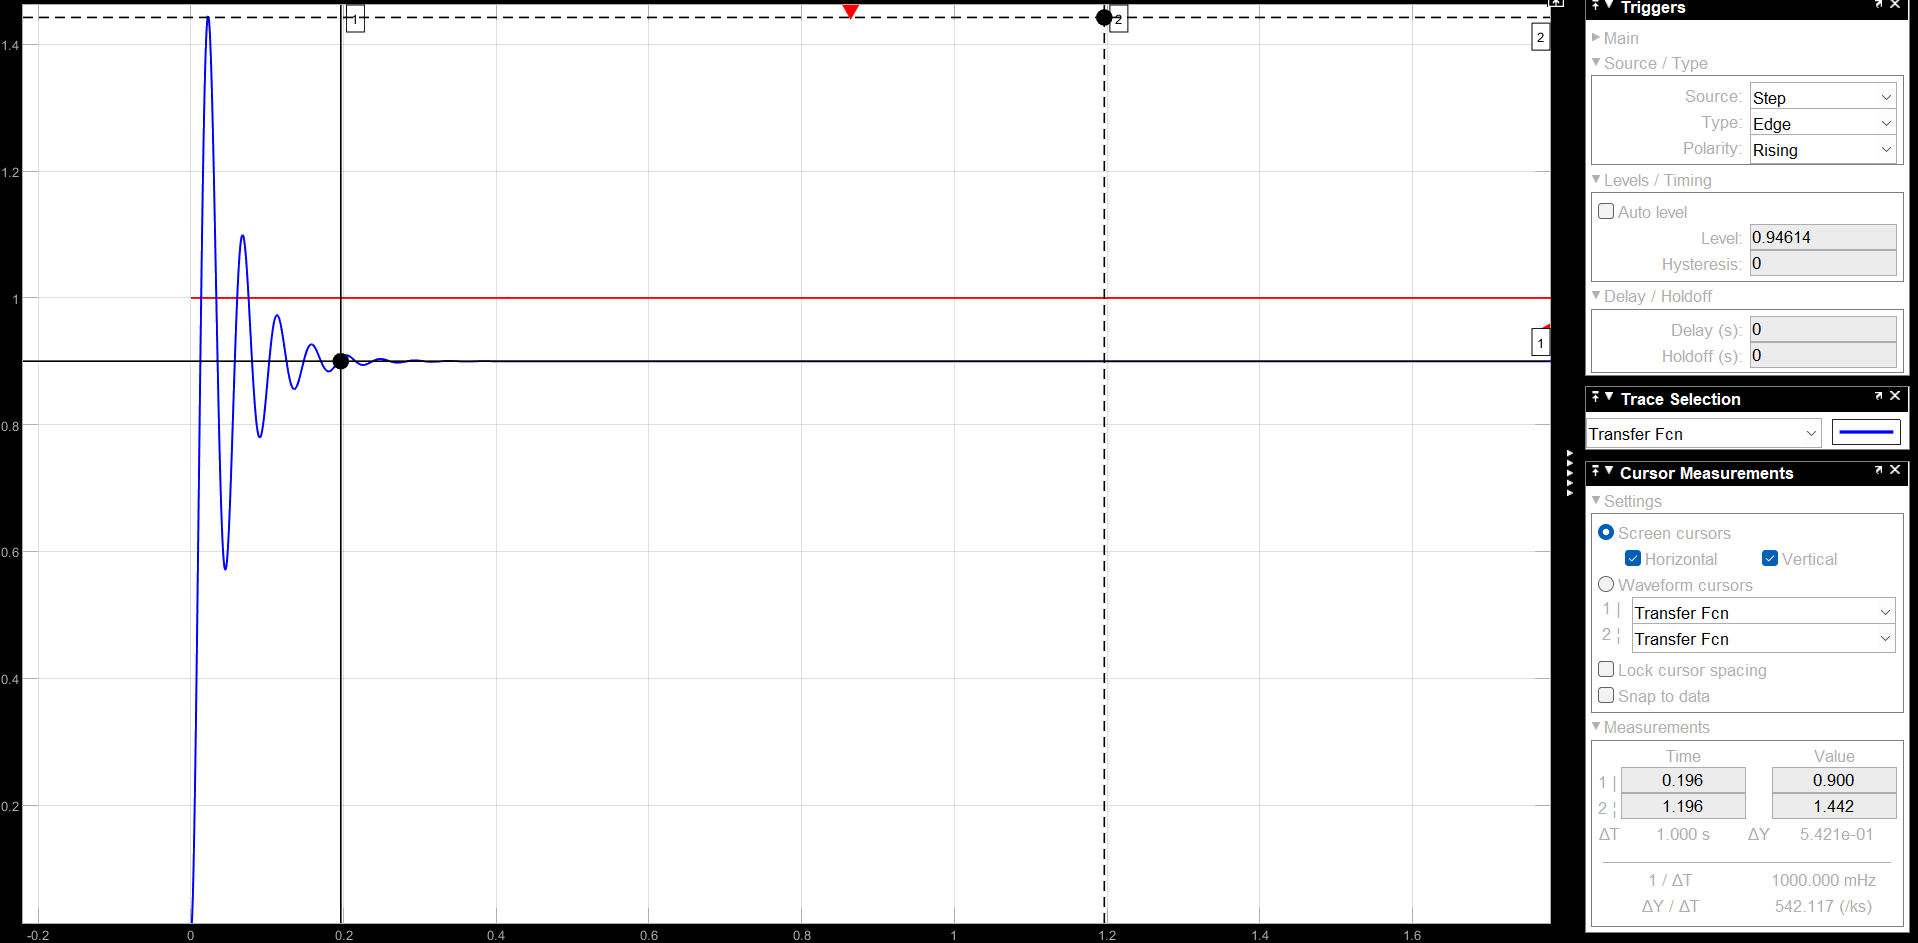
\includegraphics[width = 19 cm]{TP2 Simulink/Syst_2/Depass_4_1_K=4.5.png}
    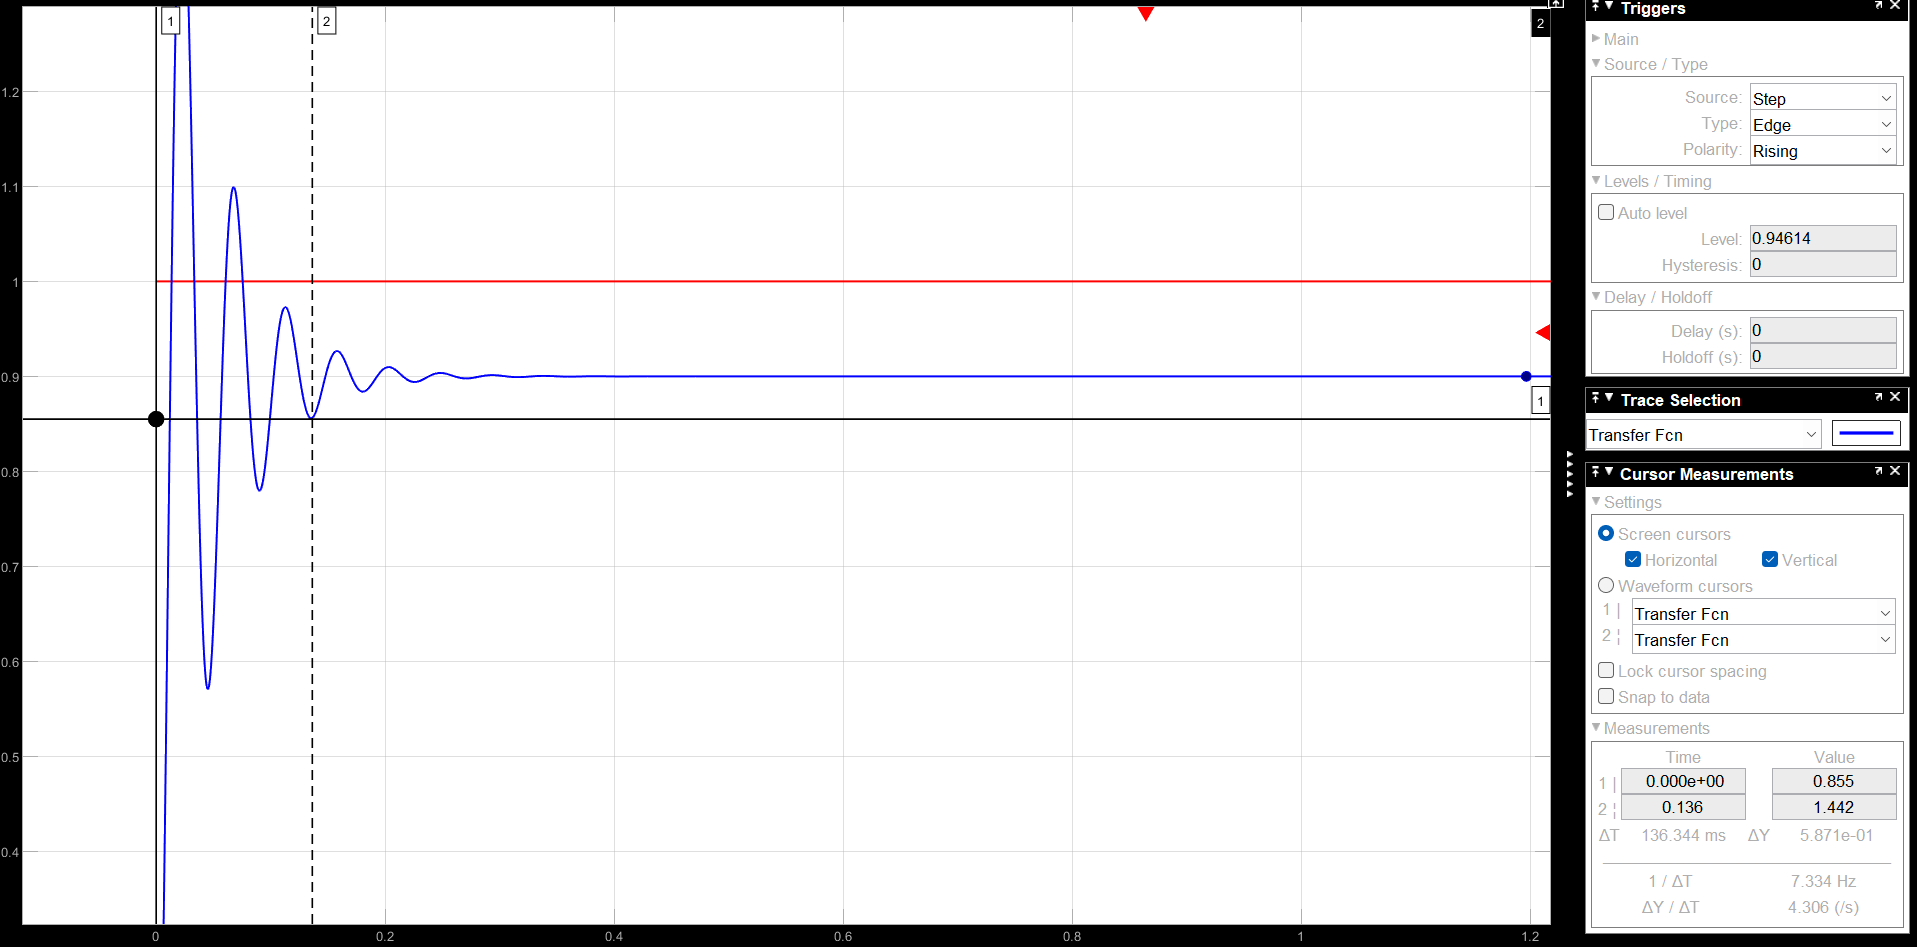
\includegraphics[width = 19 cm]{TP2 Simulink/Syst_2/tr5prct_4_1_K=4.5.png}
\end{center}
    Sur le premier graphe, on peut déjà observer que l'erreur statique est bien de 10$\%$ : l'échelon atteint 1 et la réponse indicielle 0.9, on a bien 10$\%$ d'erreur statique.
    Pour l'amplitude du premier dépassement, on détermine déjà l'écart entre le régime permanent et le dépassement : $1.442 -0.9 = 0.542$. On divise ensuite ce nombre par 1$\%$ de 0.9 donc par 0.009.
    On a finalement $D_1 = \frac{0.542}{0.009} = 60.22\%$. Enfin, on peut voir le temps de réponse à 5$\%$ sur la deuxième capture : $t_{r5\%}$ = 136.44 ms.
    Ainsi nos valeurs simulées sont plutôt proches les unes des autres (écart de 0.3$\%$ entre les valeurs des amplitudes du premier dépassement, écart nul entre les erreurs statiques et écart de 4$\%$ entre les temps de réponse). Toutes ces erreurs peuvent être dues à une imprécision des mesures sur les graphes des réponses indicielles mais comme ces erreurs ne sont pas grandes et cohérentes, le modèle est bon pour cette valeur de K.
\newpage
\begin{itemize}
    \item \bf \large K = 24.5
\end{itemize}
\begin{center}
    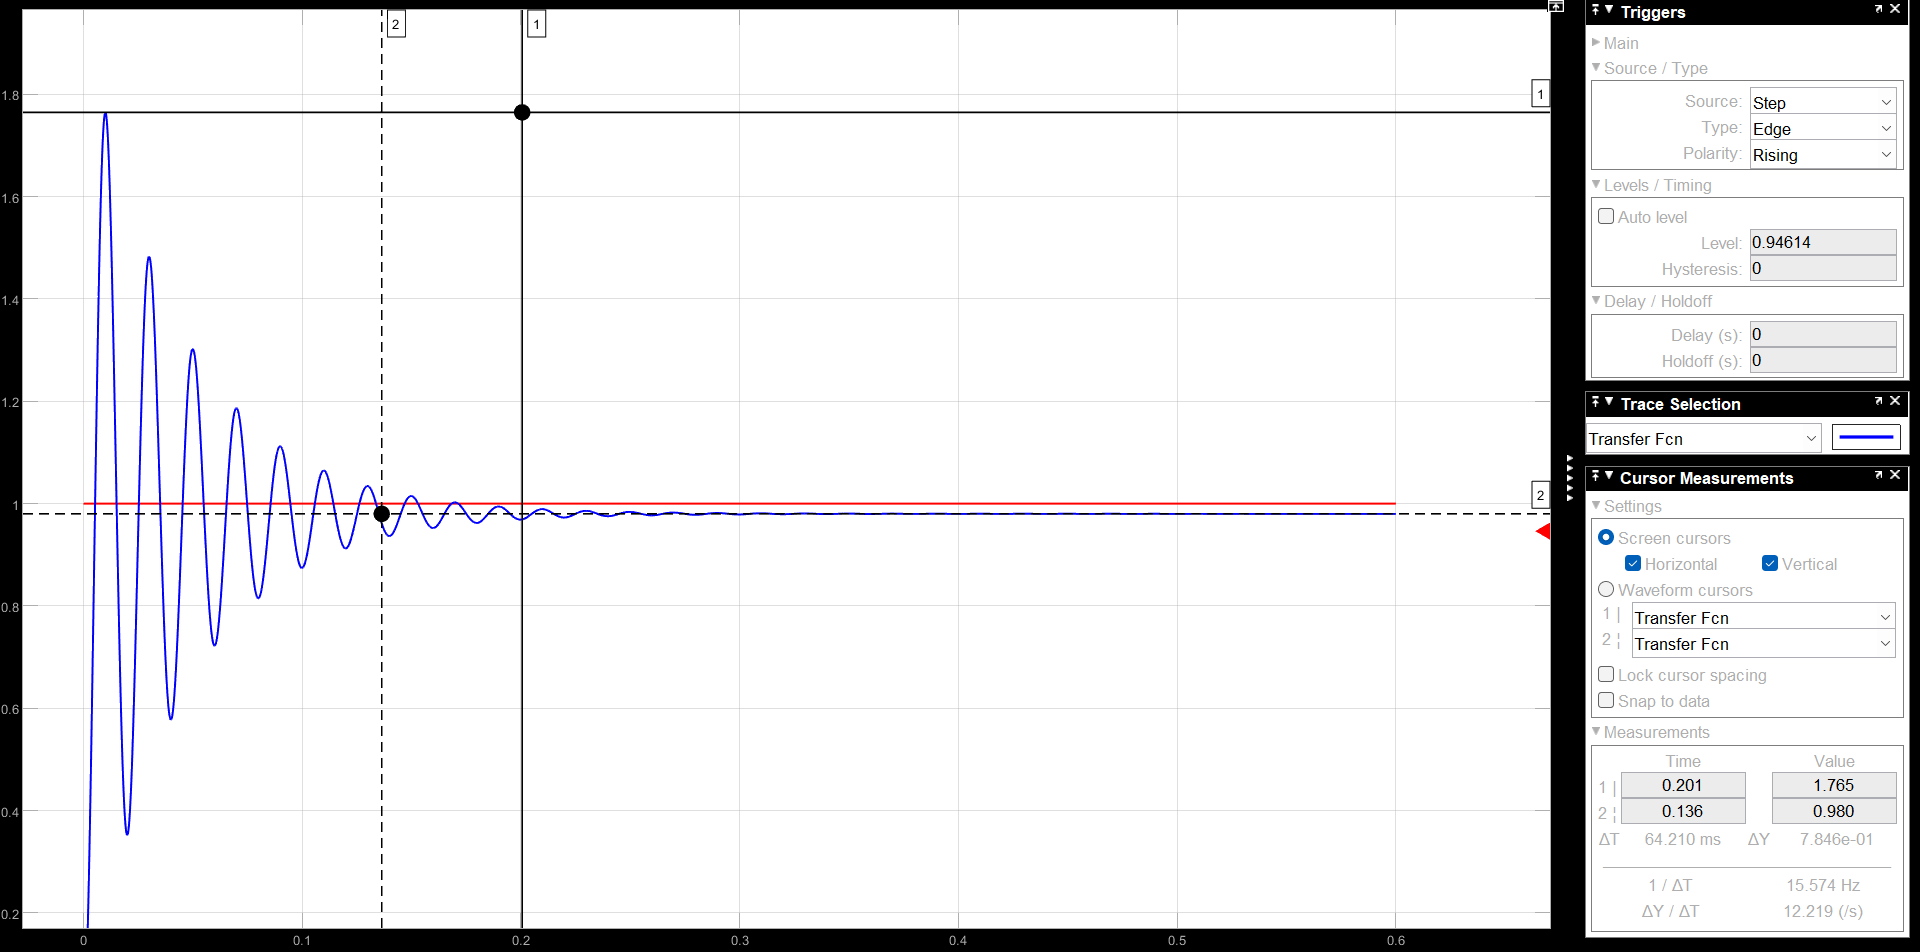
\includegraphics[width = 19 cm]{TP2 Simulink/Syst_2/depassement_4_1_K=24.5.png}
    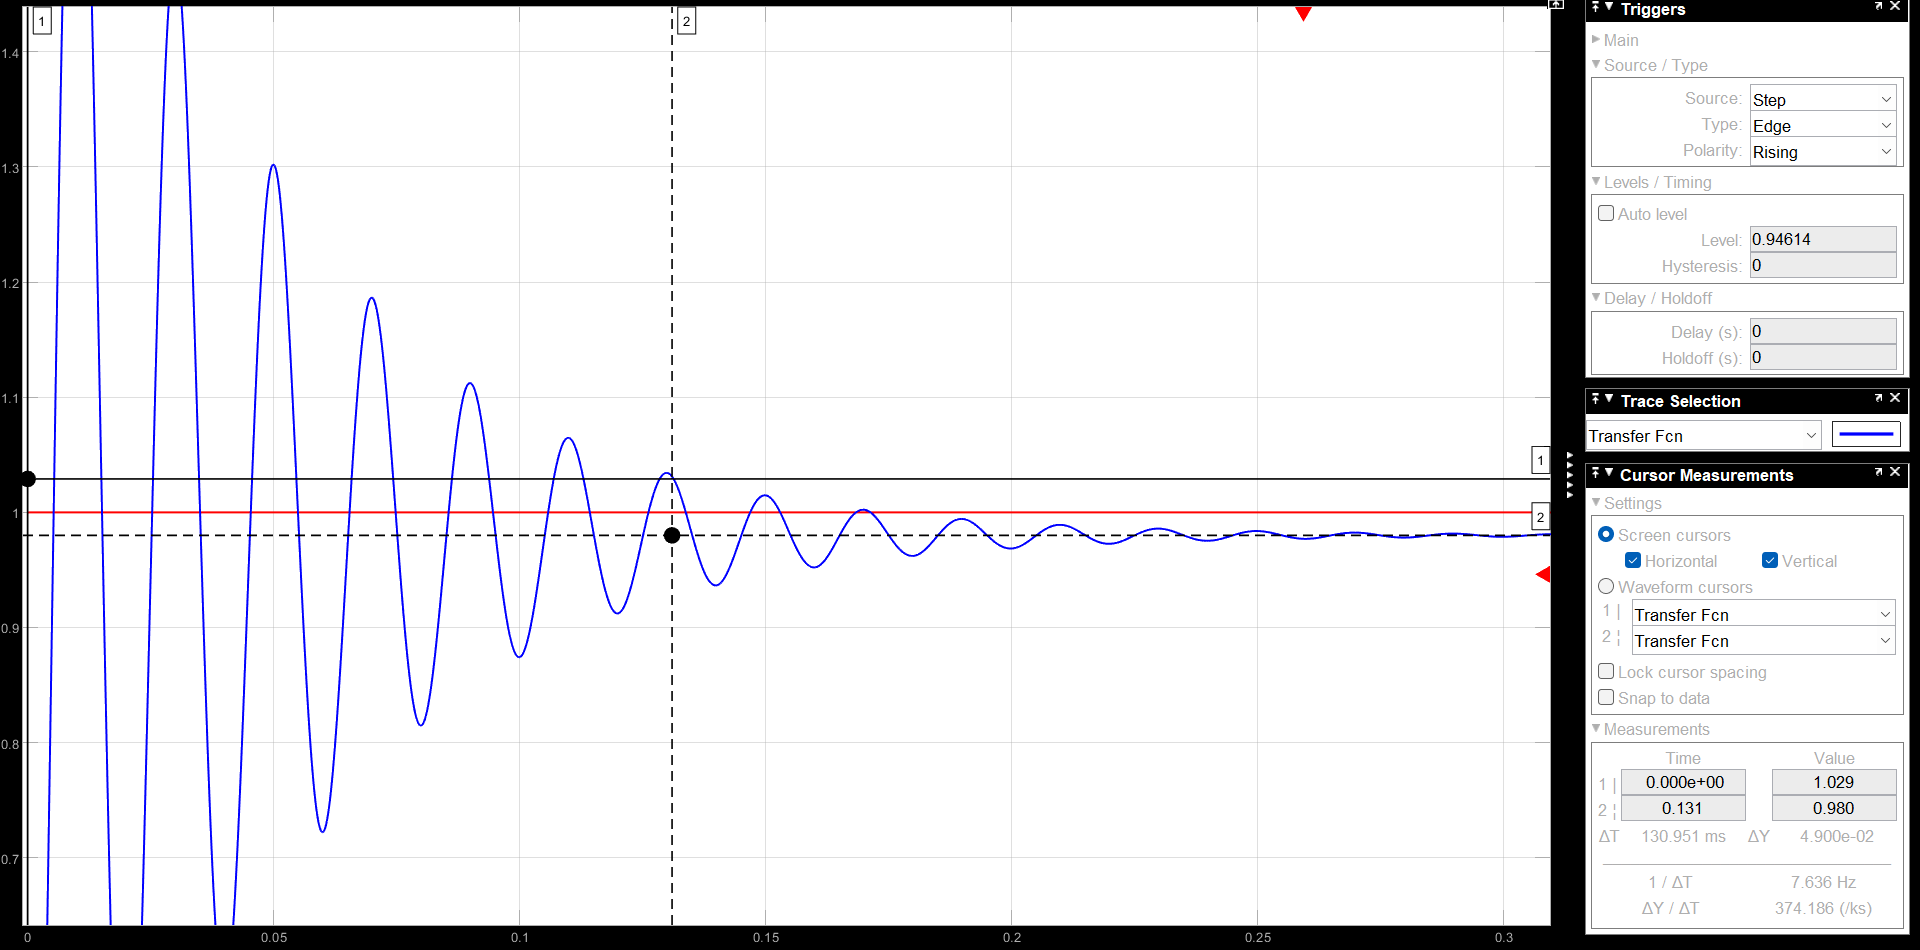
\includegraphics[width = 19 cm]{TP2 Simulink/Syst_2/tr5prct_4.1_K=24.5.png}
\end{center}
    Sur le premier graphe, on peut déjà observer que l'erreur statique est bien de 2$\%$ : l'échelon atteint 1 et la réponse indicielle 0.98, on a bien 2$\%$ d'erreur statique.
    Pour l'amplitude du premier dépassement, on détermine déjà l'écart entre le régime permanent et le dépassement : $1.765 -0.98 = 0.785$. On divise ensuite ce nombre par 1$\%$ de 0.98 donc par 0.0098.
    On a finalement $D_1 = \frac{0.785}{0.0098} = 80.10\%$. Enfin, on peut voir le temps de réponse à 5$\%$ sur la deuxième capture : $t_{r5\%}$ = 130.95 ms.
    Ainsi nos valeurs simulées sont plutôt proches les unes des autres (écart de 0.13$\%$ entre les valeurs des amplitudes du premier dépassement, écart nul entre les erreurs statiques et écart de 3.27$\%$ entre les temps de réponse). Toutes ces erreurs peuvent être dues à une imprécision des mesures sur les graphes des réponses indicielles mais comme ces erreurs ne sont pas grandes et cohérentes, le modèle est bon pour cette valeur de K.
\\\\Finalement, on se rend compte ici que plus K augmente, plus l'erreur statique diminue, mais en contrepartie le système devient plus nerveux. Dans notre cas, des dépassements de 60 et 80$\%$ sont très mauvais, malgré l'erreur statique faible.
\newpage
\subsubsection{\underline{\bf Correcteur intégral}}

On considère désormais un correcteur intégral $C(p) = \frac{1}{T_ip}$
\\\\\large \textit{ \textbf{Simulation}} 
\\\\\normalsize Le système simulé dans Simulink est relativement le même que pour le correcteur proportionnel : 
\begin{center}
    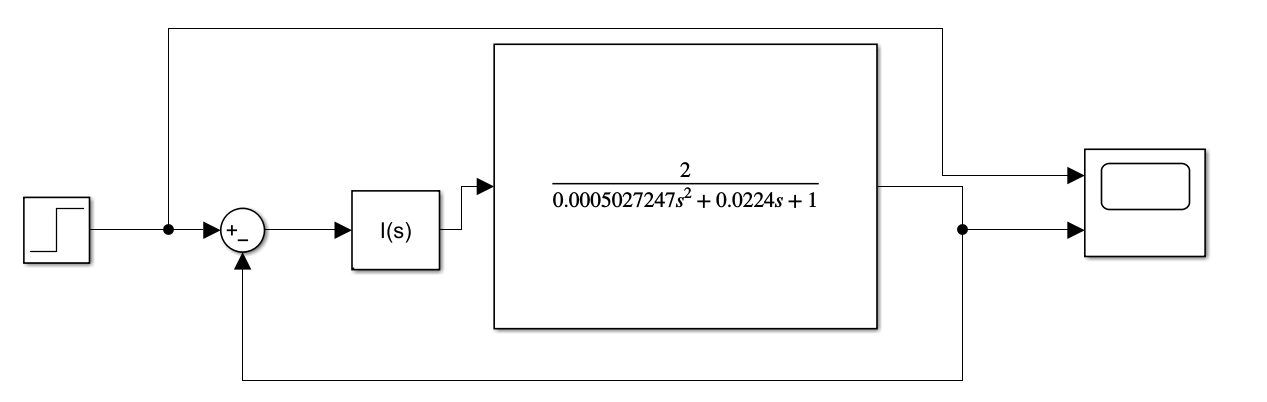
\includegraphics[width = 15 cm]{TP2 Simulink/Syst_2/Syst_2_Simulink_I.png}
\end{center}

Traçons désormais les réponses indicielles pour différentes valeurs de $T_i$ : 
\begin{itemize}
    \item \large $\mathbf{T_i = \frac{20}{\omega_0} = 0.448}$
\end{itemize}

\begin{center}
    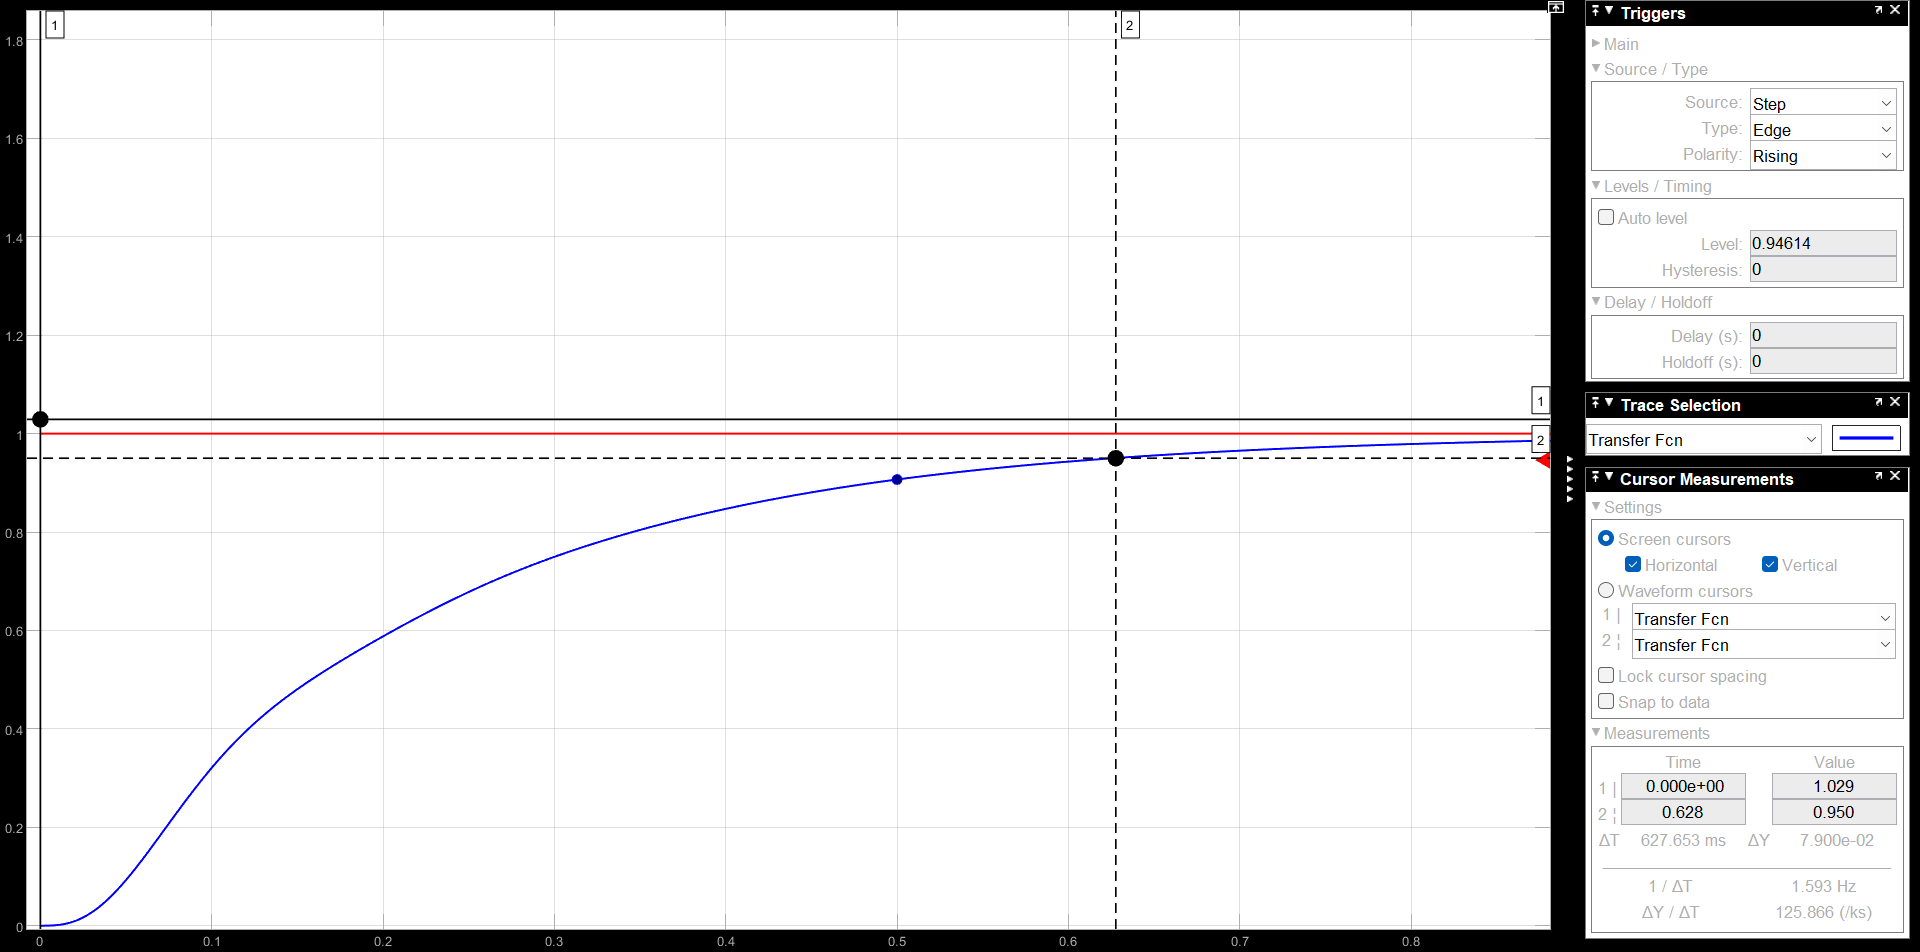
\includegraphics[width = 19 cm]{TP2 Simulink/Syst_2/tr5prct_4.2_Ti=20_sur_omega0.png}

\end{center}
On peut tout de suite remarquer que cette réponse indicielle n'admet pas de dépassements, qu'elle est bien au moins du deuxième ordre (tangente nulle à l'origine) et que l'erreur statique est nulle (elle l'est bien, il aurait fallu allonger la durée de simulation pour bien observer que la réponse tend vers 1).
On peut ensuite lire que $t_{r5\%} = 627.65$ms.

\underline{\bf Diagramme de Black de la FTBO :}
\\\\On rappelle que : 
\begin{center}
   \large $FTBO = \frac{A}{T_ip + \frac{2zT_i}{\omega_0}p^2 + \frac{T_i}{\omega_0^2}p^3}$.
    \normalsize Pour $T_i = \frac{20}{\omega_0}$, \large $FTBO = \frac{2}{0.4484p + 0.101p^2 + 0.0002254p^3}$.
\end{center}
\normalsize On obtient alors :
\begin{center}
    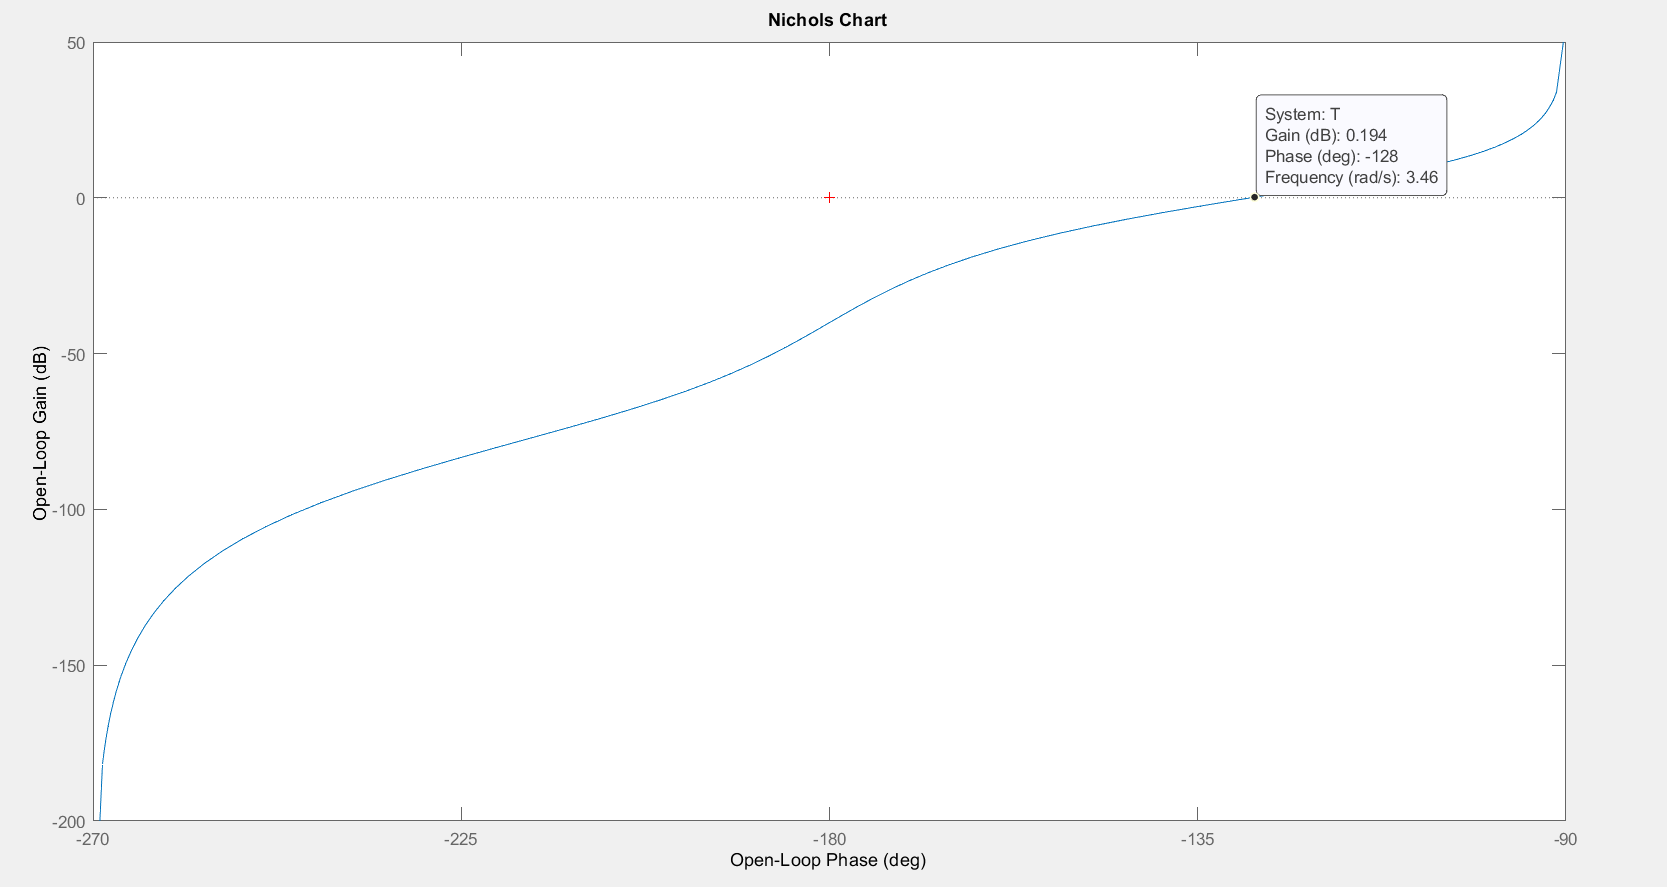
\includegraphics[width = 19 cm]{TP2 Simulink/Syst_2/nichols_Ti=20_sur_omega0.png}
\end{center}
On trouve comme marge de phase \fbox{$m_{\phi_{\frac{20}{\omega_0}}} = -128-(-180) = 52^{\circ}$}.
\newpage
\begin{itemize}
    \item \large $\mathbf{T_i = \frac{10}{\omega_0} = 0.2242}$
\end{itemize}
\begin{center}
    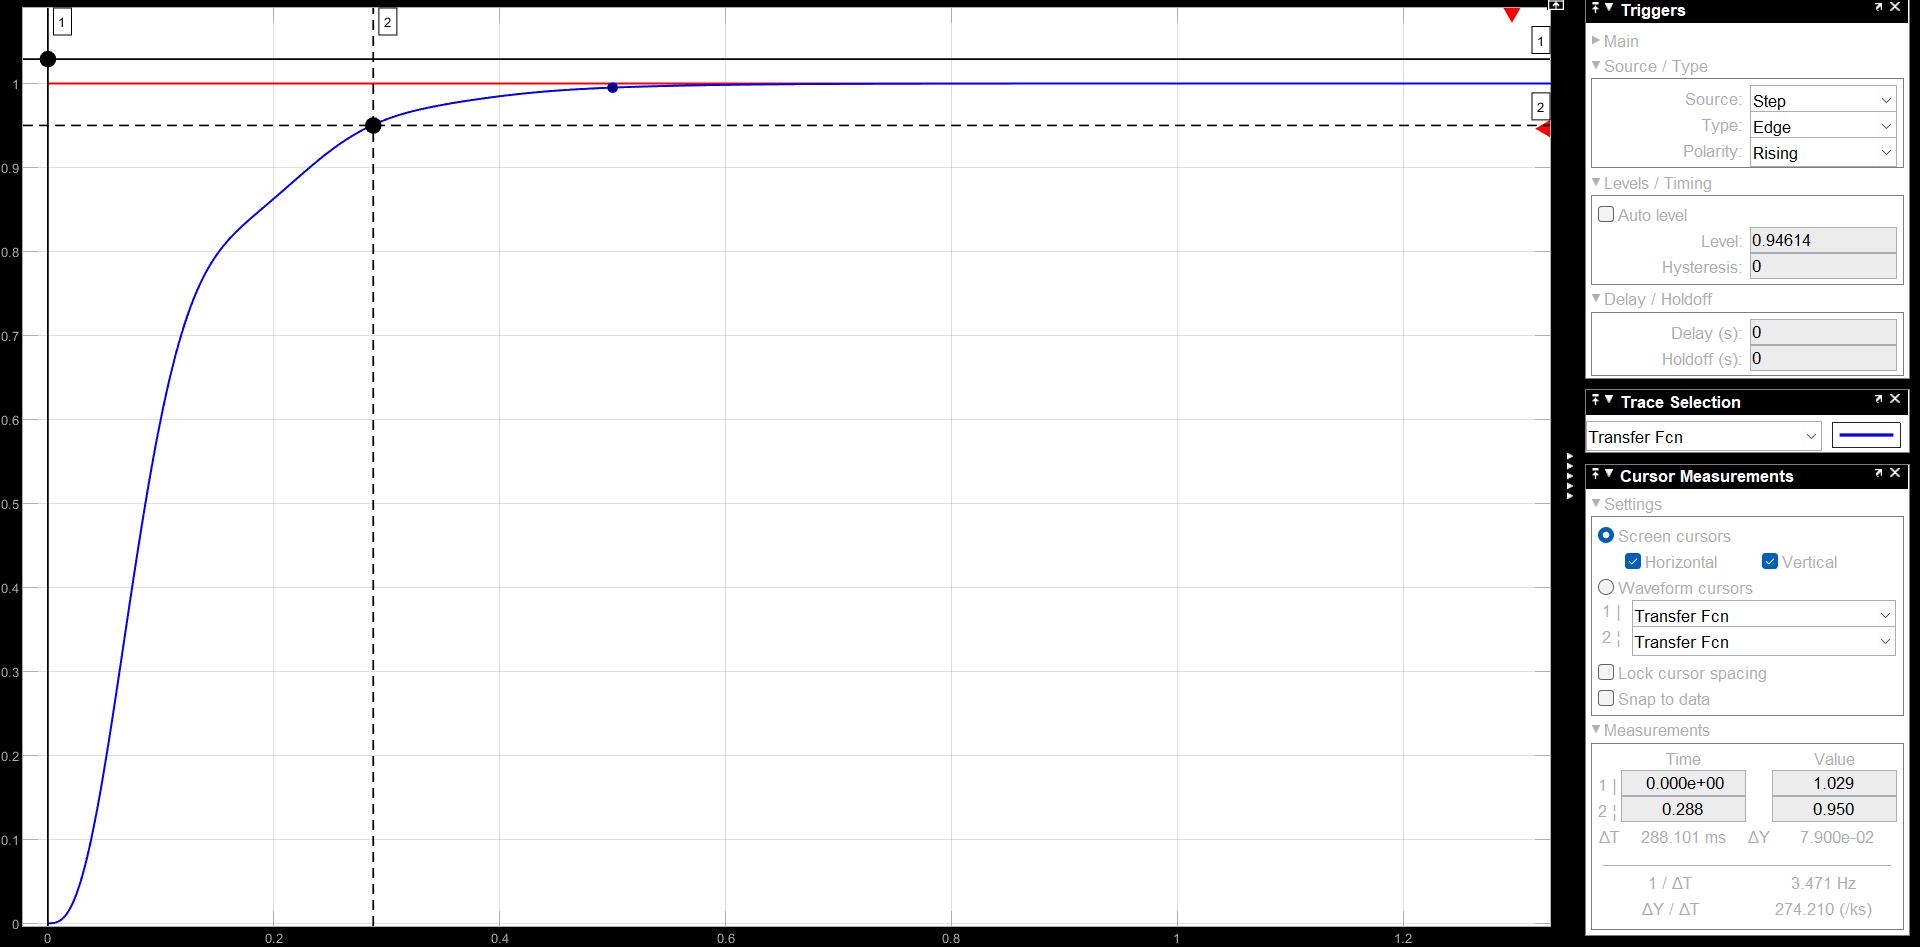
\includegraphics[width = 19 cm]{TP2 Simulink/Syst_2/tr5prct_4.2_Ti=10_sur_omega0.png}

\end{center}
On peut de nouveau remarquer que cette réponse indicielle n'admet pas de dépassements, qu'elle est bien au moins du deuxième ordre (tangente nulle à l'origine) et que l'erreur statique est nulle.
On peut ensuite lire que $t_{r5\%} = 288.10$ms.
\\\\\underline{\bf Diagramme de Black de la FTBO :}

\begin{center}
    \normalsize Pour $T_i = \frac{10}{\omega_0}$, \large $FTBO = \frac{2}{0.2242p + 0.00503p^2 + 0.0001127p^3}$.
\end{center}
\newpage
\normalsize On obtient alors :
\begin{center}
    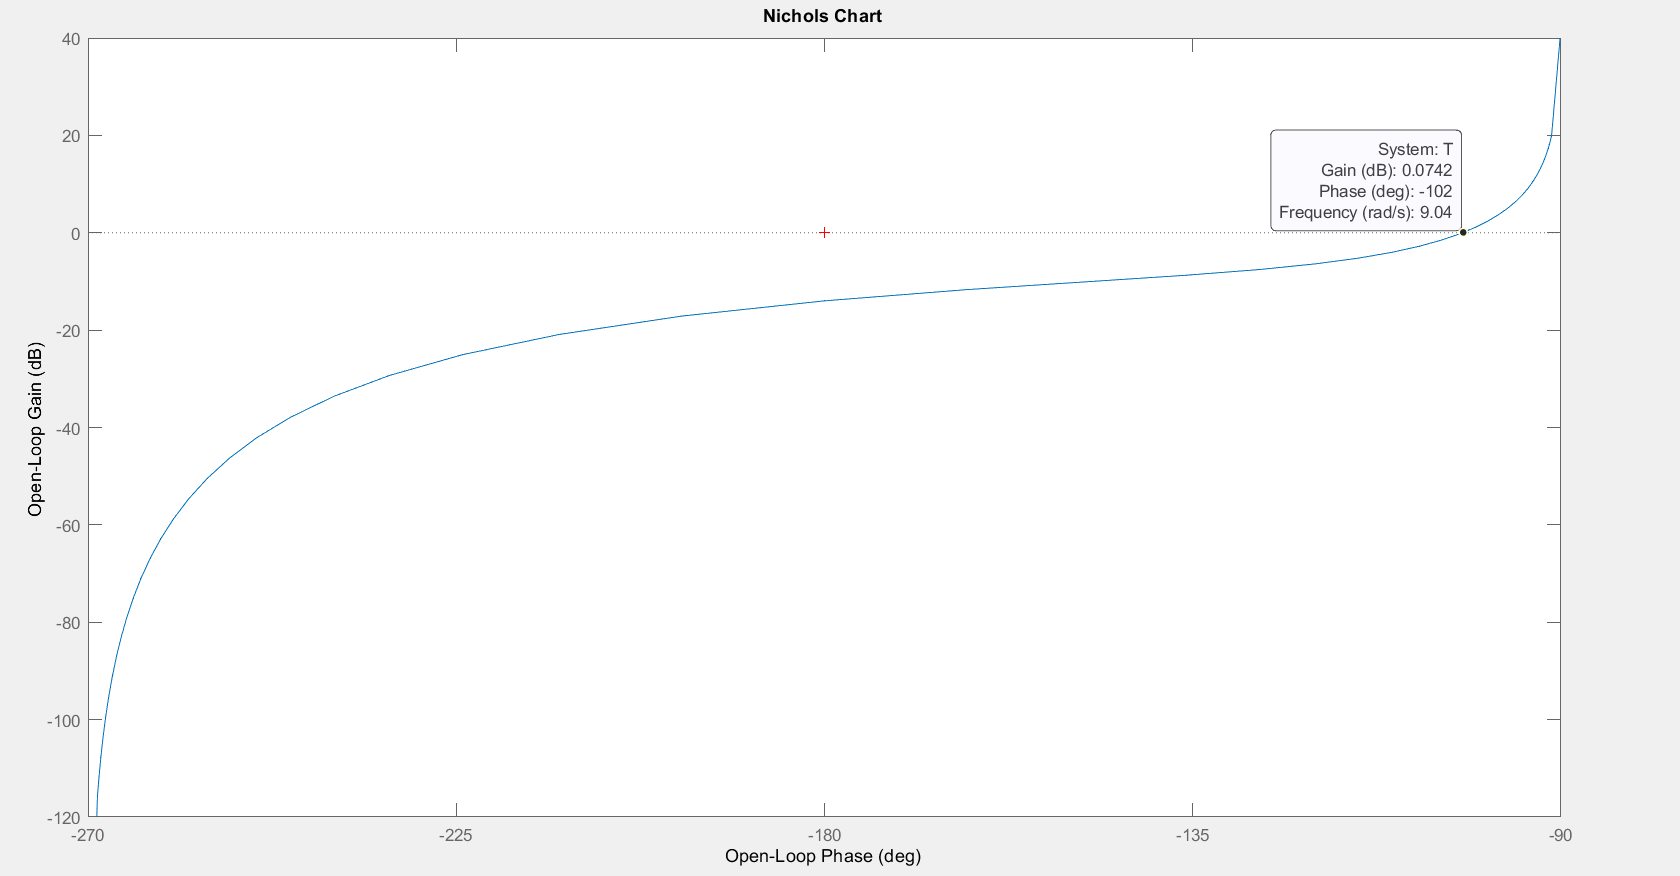
\includegraphics[width = 19 cm]{TP2 Simulink/Syst_2/nichols_Ti=10_sur_omega0.png}
\end{center}
On trouve comme marge de phase \fbox{$m_{\phi_{\frac{10}{\omega_0}}} = -102-(-180) = 78^{\circ}$}.
\newpage
\begin{itemize}
    \item \large $\mathbf{T_i = \frac{5}{\omega_0} = 0.112}$
\end{itemize}
\begin{center}
    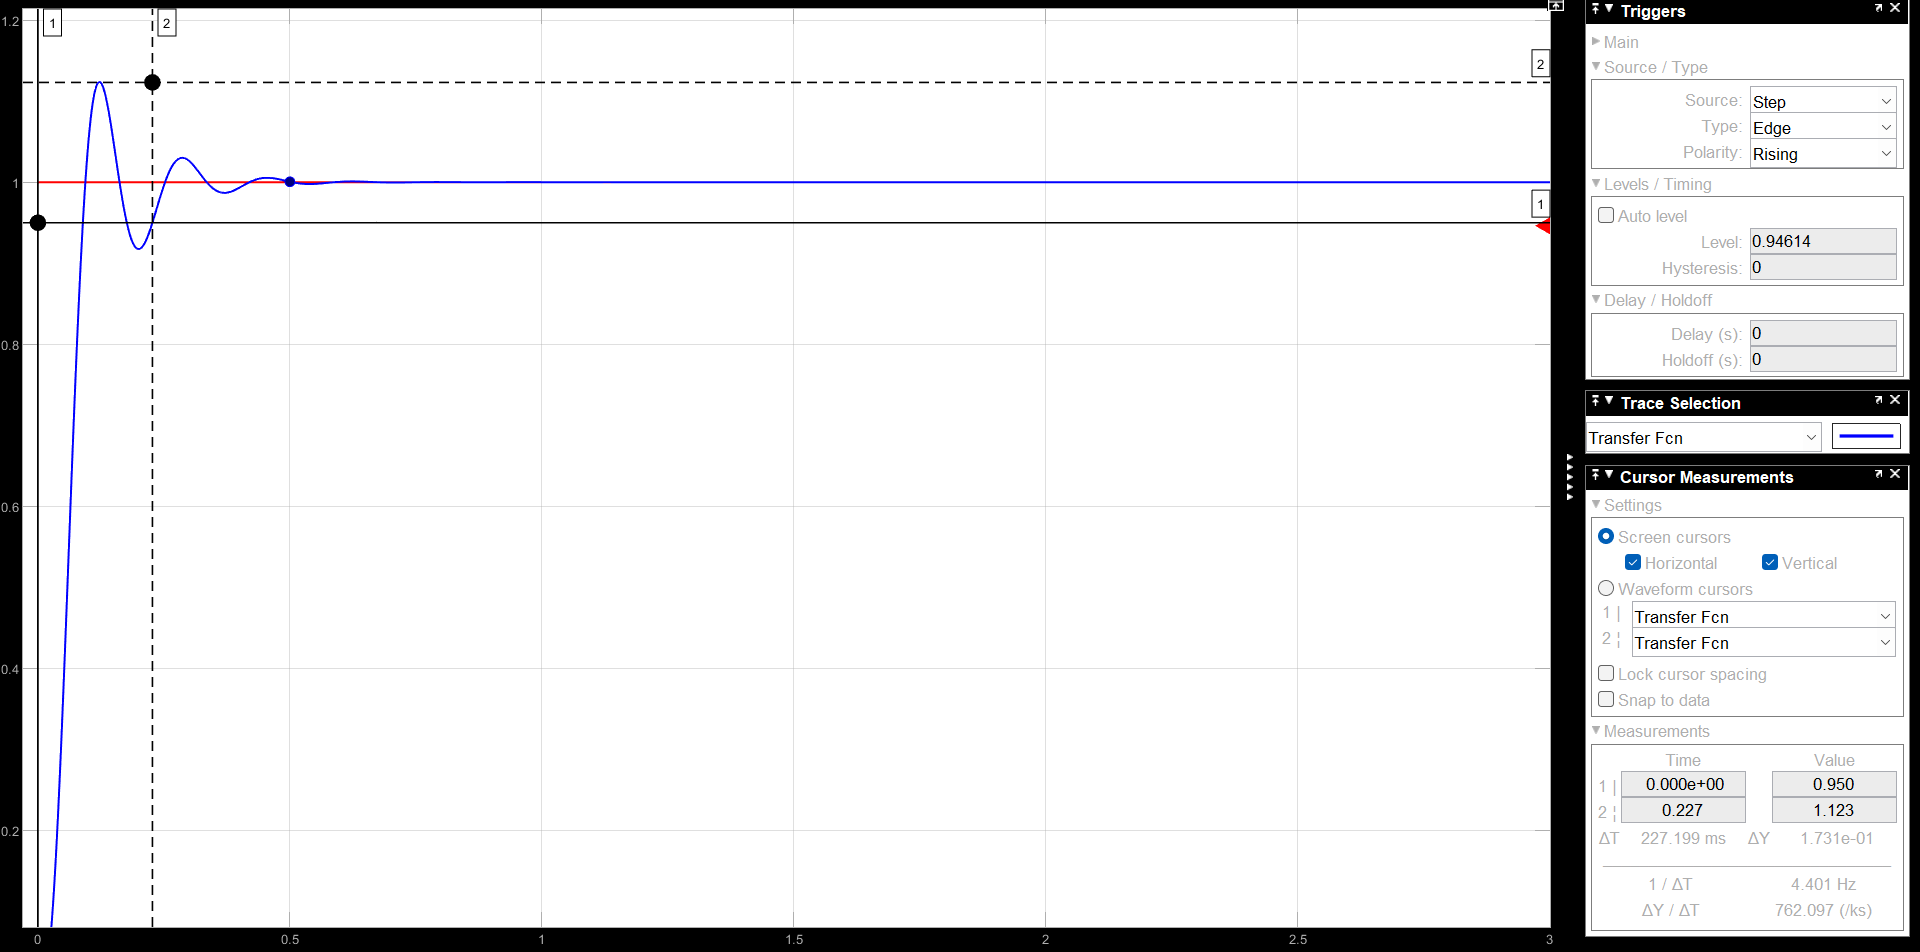
\includegraphics[width = 19 cm]{TP2 Simulink/Syst_2/tr5prct_et_depassement_4.2_5_sur_omega0.png}

\end{center}
On remarque que la réponse admet désormais des dépassements, mais l'erreur staituqe est toujours nulle. Nous avons placé les curseurs de façon à pouvoir mesurer l'amplitude du premier dépassement et le temps de réponse à cinq pourcents.
On trouve ainsi $D_1 = 12.3\%$ et $t_{r5\%} = 227.2$ms.
\\\\\underline{\bf Diagramme de Black de la FTBO :}

\begin{center}
    \normalsize Pour $T_i = \frac{5}{\omega_0}$, \large $FTBO = \frac{2}{0.1121p + 0.0025p^2 + 0.0000564p^3}$.
\end{center}
\newpage
\normalsize On obtient alors :
\begin{center}
    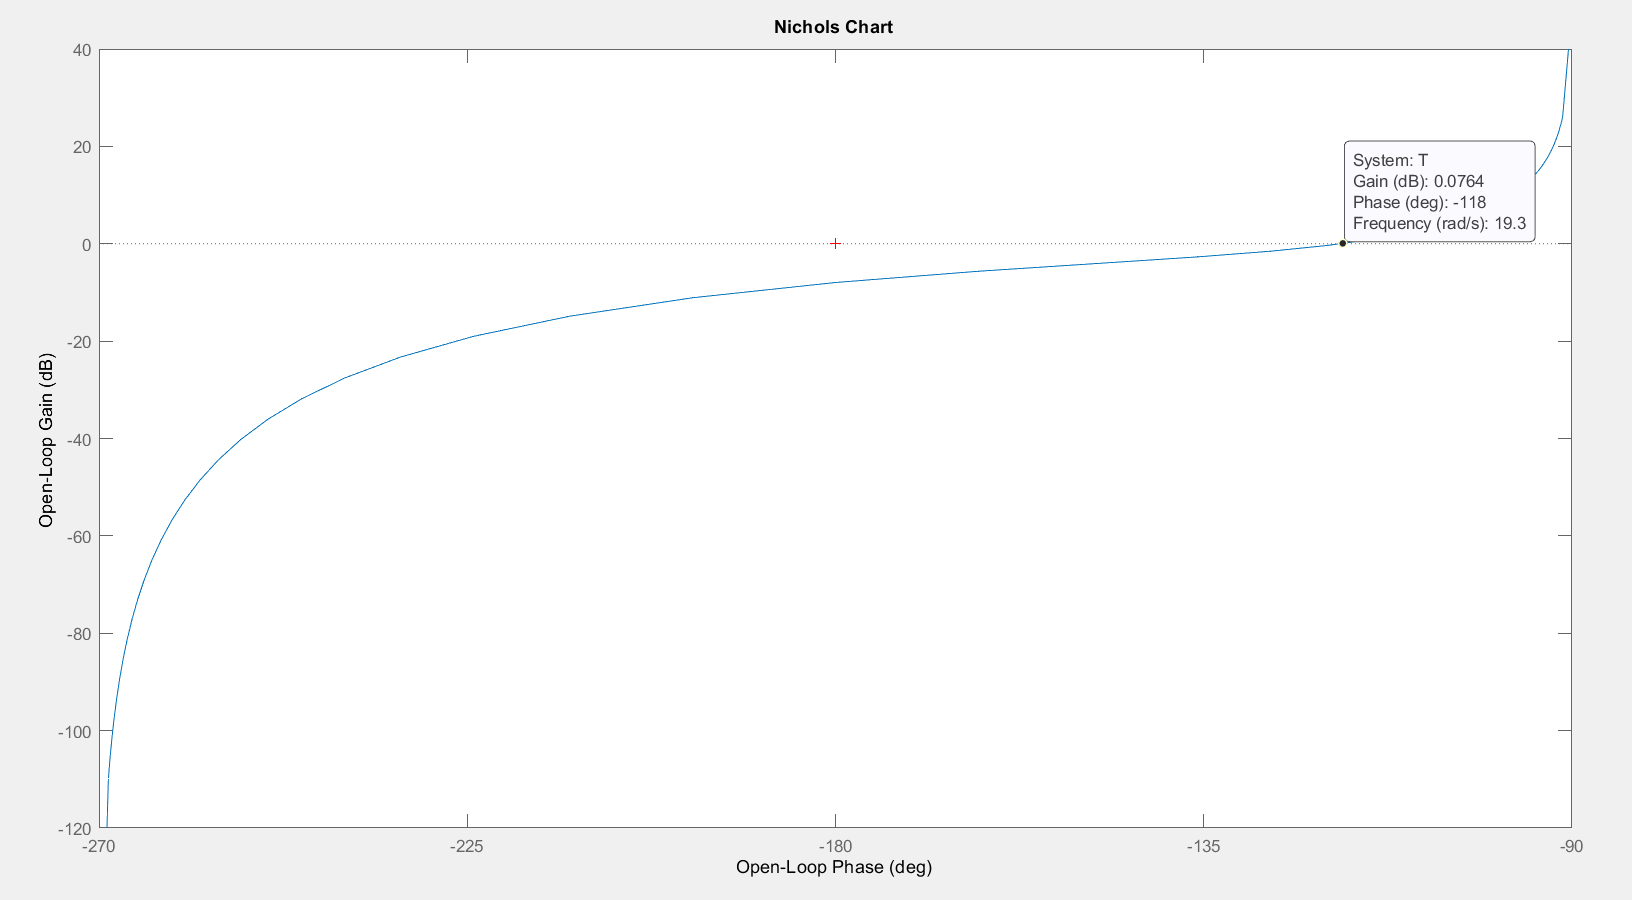
\includegraphics[width = 19 cm]{TP2 Simulink/Syst_2/nichols_4.2_Ti=5_sur_omega0.png}
\end{center}
On trouve comme marge de phase \fbox{$m_{\phi_{\frac{5}{\omega_0}}} = -118-(-180) = 62^{\circ}$}.
\newpage
\begin{itemize}
    \item \large $\mathbf{T_i = \frac{1}{\omega_0} = 0.02242}$
\end{itemize}
\begin{center}
    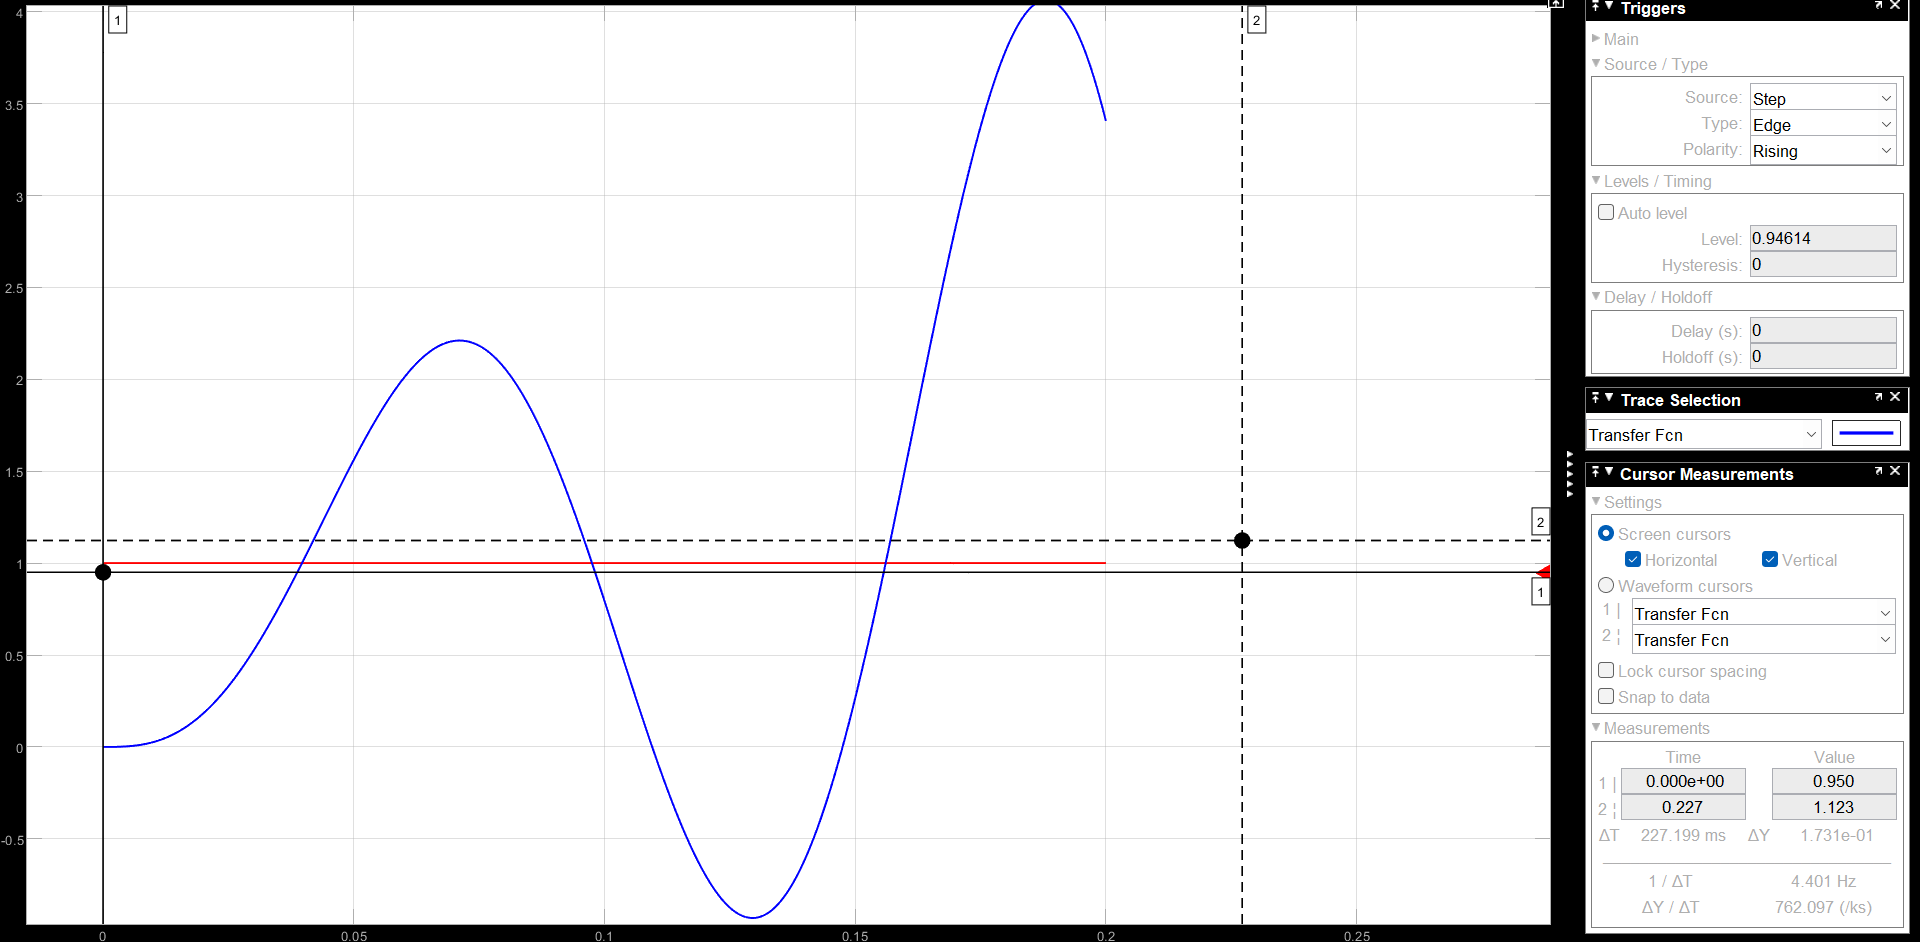
\includegraphics[width = 19 cm]{TP2 Simulink/Syst_2/4.2_instable_Ti=1_sur_omega0.png}


\end{center}
Pour cette valeur de $T_i$, le système est instable. On peut le confirmer en mesurant la marge de phase :
\\\\\underline{\bf Diagramme de Black de la FTBO :}

\begin{center}
    \normalsize Pour $T_i = \frac{1}{\omega_0}$, \large $FTBO = \frac{2}{0.0224p + 0.000503p^2 + 0.0000113p^3}$.
\end{center}
\newpage
\normalsize On obtient alors :
\begin{center}
    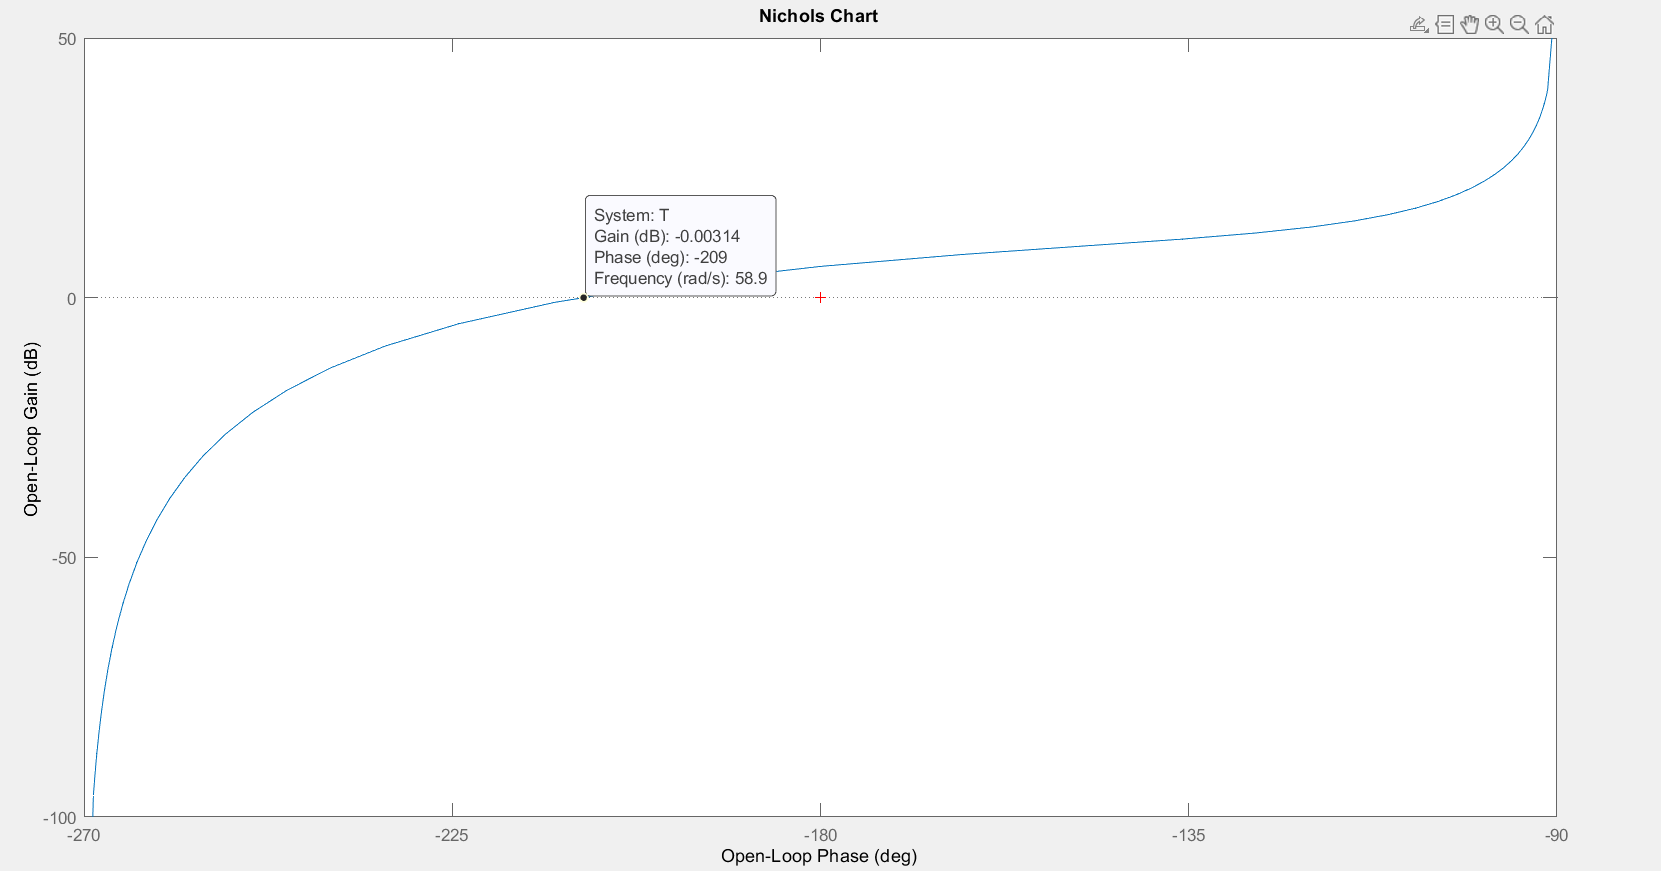
\includegraphics[width = 19 cm]{TP2 Simulink/Syst_2/nichols_4.2_Ti=1_sur_omega0.png}
\end{center}
On trouve comme marge de phase \fbox{$m_{\phi_{\frac{1}{\omega_0}}} = -209-(-180) = -29^{\circ} < 0$}. Le système est donc bien instable.

\end{document}